\documentclass[10pt]{article}
\usepackage[letterpaper]{geometry}
\geometry{verbose,tmargin=1in,bmargin=1in,lmargin=1in,rmargin=1in}
\usepackage{setspace}
\usepackage{ragged2e}
\usepackage{color}
\usepackage{titlesec}
\usepackage{graphicx}
\usepackage{float}
\usepackage{mathtools}
\usepackage{amsmath}
\usepackage[font=small,labelfont=bf,labelsep=period]{caption}
\usepackage[english]{babel}
\usepackage{indentfirst}
\usepackage{array}
\usepackage{makecell}
\usepackage[usenames,dvipsnames]{xcolor}
\usepackage{multirow}
\usepackage{tabularx}
\usepackage{arydshln}
\usepackage{caption}
\usepackage{subcaption}
\usepackage{xfrac}
\usepackage{etoolbox}
\usepackage{cite}
\usepackage{url}
\usepackage{dcolumn}
\usepackage{hyperref}
\usepackage{courier}
\usepackage{url}
\usepackage{esvect}
\usepackage{commath}
\usepackage{verbatim} % for block comments
\usepackage{enumitem}
\usepackage{hyperref} % for clickable table of contents
\usepackage{braket}
\usepackage{titlesec}
\usepackage{booktabs}
\usepackage{gensymb}
\usepackage{longtable}
\usepackage{soul} % for striking out text
\usepackage{tcolorbox} % for colored boxes
\tcbuselibrary{breakable} % to allow colored boxed to extend over multiple pages
\usepackage[makeroom]{cancel}	% to cancel out text
\usepackage{breqn}
\usepackage[mathscr]{euscript}
\usepackage[acronym,nomain,nonumberlist,nogroupskip,nopostdot]{glossaries} % for glossary of acronyms

% for circled numbers
\usepackage{tikz}
\newcommand*\circled[1]{\tikz[baseline=(char.base)]{
            \node[shape=circle,draw,inner sep=2pt] (char) {#1};}}

\newcommand{\beq}{\begin{equation}}
\newcommand{\eeq}{\end{equation}}
\newcommand{\beqa}{\begin{equation}\begin{aligned}}
\newcommand{\eeqa}{\end{aligned}\end{equation}}
\newcommand{\hO}{\hat{\Omega}}
\newcommand{\Om}{\Omega}
\newcommand{\spa}{(\vv{r}, E, \hO, t)}
\newcommand{\seat}{(\vv{r}, E, \hO, t)}
\newcommand{\seatelse}{(\vv{r},E',\hO',t)}
\newcommand{\sat}{(\vv{r},\hO,t)}
\newcommand{\sset}{(\vv{r},E,t)}
\newcommand{\seatprime}{(\vv{r},E',\hO',t)}
\newcommand{\seatout}{(\vv{r},E'\rightarrow E,\hO'\rightarrow \hO,t)}
\newcommand{\spas}{(\vv{r},E,t)}
\newcommand{\spap}{(\vv{r}, E', \hO',t)}
\newcommand{\spaps}{(\vv{r},E',t)}
\newcommand{\spang}{(\vv{r},E'\rightarrow E, \hO'\rightarrow\hO,t)}
\newcommand{\spangr}{(\vv{r},E\rightarrow E', \hO\rightarrow\hO',t)}
\newcommand{\dEprime}{\int_{0}^\infty dE'}
\newcommand{\dhOprime}{\int_{4\pi}d\hO'}

% integrand (minus the flux) of the prompt fission source
\newcommand{\promptfissionsource}{\chi_p(E,\hO)\dEprime\dhOprime\left\lbrack1-\beta(E')\right\rbrack\nu(E')\Sigma_f\seatprime}

% summation form of the delayed neutron source
\newcommand{\delayedfissionsource}{\sum_{j=1}^J\chi_{d,j}(E,\hO)\lambda_jC_j(\vv{r},t)}

% total fission source
\newcommand{\totalfissionsource}{\chi(E,\hO)\int_0^\infty dE'\int_{4\pi}d\hO' \nu(E')\Sigma_f\seatprime}

% in-scattering source
\newcommand{\inscatteringsource}{\int_0^\infty dE'\int_{4\pi}d\hO'\Sigma_s\seatout}

% external source
\newcommand{\source}{S\seat}

\titleclass{\subsubsubsection}{straight}[\subsection]

% define new command for triple sub sections
\newcounter{subsubsubsection}[subsubsection]
\renewcommand\thesubsubsubsection{\thesubsubsection.\arabic{subsubsubsection}}
\renewcommand\theparagraph{\thesubsubsubsection.\arabic{paragraph}} % optional; useful if paragraphs are to be numbered

\titleformat{\subsubsubsection}
  {\normalfont\normalsize\bfseries}{\thesubsubsubsection}{1em}{}
\titlespacing*{\subsubsubsection}
{0pt}{3.25ex plus 1ex minus .2ex}{1.5ex plus .2ex}

\makeatletter
\renewcommand\paragraph{\@startsection{paragraph}{5}{\z@}%
  {3.25ex \@plus1ex \@minus.2ex}%
  {-1em}%
  {\normalfont\normalsize\bfseries}}
\renewcommand\subparagraph{\@startsection{subparagraph}{6}{\parindent}%
  {3.25ex \@plus1ex \@minus .2ex}%
  {-1em}%
  {\normalfont\normalsize\bfseries}}
\def\toclevel@subsubsubsection{4}
\def\toclevel@paragraph{5}
\def\toclevel@paragraph{6}
\def\l@subsubsubsection{\@dottedtocline{4}{7em}{4em}}
\def\l@paragraph{\@dottedtocline{5}{10em}{5em}}
\def\l@subparagraph{\@dottedtocline{6}{14em}{6em}}
\makeatother

\newcommand{\volume}{\mathop{\ooalign{\hfil$V$\hfil\cr\kern0.08em--\hfil\cr}}\nolimits}

\setcounter{secnumdepth}{4}
\setcounter{tocdepth}{4}

\setacronymstyle{long-short}
\loadglsentries{../../projects/pronghorn/doc/manual/manual_glossary}
\makeglossaries

\begin{document}

\begin{centering}
\textbf{\Large Neutron Transport}\\
\end{centering}

\tableofcontents
\clearpage

\section{Introduction}
\begin{flushleft}\justify

This document will cover the two main models for neutron populations, beginning with transport theory, and then moving to a simplification known as diffusion theory. While diffusion theory is a very accurate approximation to heat conduction or gaseous diffusion where ``random-walk'' physical processes occur frequently, it is less accurate for describing neutron populations. Due to the uncharged nature of neutrons and their sometimes fairly low interaction probabilities with the material in which they are traveling, neutrons can travel long distances without any interaction, which degrades a ``random-walk'' assumption. The interaction of a neutron population with a domain is governed by interaction probabilities. Naturally, these probabilities are functions of neutron energy, space (if the domain is heterogeneous), and time (if the domain is time-dependent). In addition, because neutrons are particles, their direction of travel also has an impact on their likelihood to undergo certain interactions in heterogeneous geometries. A neutron may be very close to a highly interacting region, but if the neutron is not moving towards that region, its probability of interaction will be entirely different. So, for heterogeneous media, the breakdown in diffusion theory is most apparent near boundaries in the geometry where there are moderate to large changes in interaction probabilities within a few mean free paths. 

So, while diffusion theory represents a much simpler model of neutron populations, it is necessary to begin with a study neutron transport. The neutron transport equation is difficult to solve due to the high dimensionality of phase space and the integro-differential form of the equation. The neutron transport equation is the linear version of the general Boltzmann transport equation developed to describe gases. Despite this great reduction in complexity from the Boltzmann equation, the solution can only be obtained in the simplest of geometries. Initially, the people who worked with the Bolztmann transport equation were satisfied by only applying it in semi-infinite media, since it was used for atmospheric and stellar applications. Its application to more finite domains really began with the field of nuclear engineering. 

\clearpage
\section{The Physics of Nuclear Interactions}

This section provides the physical background needed to understand the probabilities of neutron interactions with matter. Due to the very large neutron densities on the order of \(10^8\) per cm$^3$, neutron interactions with matter will only be regarded in an average sense, as such detailed accounting of every neutron is unneccessary. 

\subsection{Radioactive Decay}
\label{sec:RadioactiveDecay}
There are four important types of radioactive decay:

\begin{enumerate}
\item Alpha decay - a nucleus emits a helium nucleus,
\item Beta decay - a neutron is converted to a proton in the nucleus, and an electron and neutrino are emitted,
\item Gamma decay - a nucleus transitions from a higher energy state to a lower energy state and in the process emits a photon, and
\item Neutron decay - a neutron is emitted
\end{enumerate}

The physics of radioactive decay are based on the assumption that the probability of decay of a nuclide is constant in time - an excellent approximation. This probability of decay per unit time, \(\lambda\) is known as the decay constant. If the probability of decay is a constant independent of the number of nuclei present or other environmental conditions, the rate of the change of the number of nuclei \(N\) is proportional to the number present:

\beq
\label{eq:Decay}
\frac{dN(t)}{dt}=-\lambda N(t)
\eeq

The quantity \(\lambda N\) represents the instantaneous number of radioactive decays occurring, and is also referred to as the activity \(A\):

\beq
\label{eq:ActivityDef}
A(t)\equiv\lambda N(t)
\eeq

Activity is typically quoted in units of Curies, or \(3.7\times10^{10}\) decays per second, roughly equivalent to the activity of one gram of radium. Solution of Eq. \eqref{eq:Decay} provides an expression for the number of nuclei present given an initial number \(N_0\):

\beq
\label{eq:DecayEqn}
N(t)=N_0e^{-\lambda t}
\eeq

Note that for systems of different nuclides, a system of equations of the form in Eq. \eqref{eq:Decay} exists with additional source terms representing decay chain effects; this constant-coefficient system can be easily solved. The instantaneous rate of radioactive decay is obtained simply by multiplying \(N(t)\) by the decay constant, from which it is clear that the probability a nuclei will decay in a time interval \(t\) to \(t+dt\) is:

\beq
\label{eq:ProbabilityDecay}
p_{\text{decay}}=\lambda e^{-\lambda t}dt
\eeq

The expectation value of the lifetime \(\bar{t}\) of a nuclide is calculated by computing the first moment of the probability of decay:

\beqa
\label{eq:MeanLifetime}
\bar{t}\equiv&\int_0^\infty dt\ t\lambda e^{-\lambda t}dt\\
=&\frac{1}{\lambda}
\eeqa

Eq. \eqref{eq:MeanLifetime} can be more intuitively understood if the probability of decay were a delta function for a specific time \(t_i\), in which case the integral in Eq. \eqref{eq:MeanLifetime} would simply equal \(t_i\), as expected. For gamma decay, a nucleus transition between two states with a difference in energies \(\Delta E\). From the Heisenberg uncertainty principle, if \(\Delta t\) is taken as the average lifetime of the higher-energy state before decaying to the lower-energy state, it is clear that \(\Delta E\propto\lambda\), so states with very large transitions in energy tend to have much larger decay constants than smaller-energy transitions.

\subsection{Nuclear Collisions}
As opposed to radioactive decay discussed in Section \ref{sec:RadioactiveDecay}, the probabilities of nuclear collisions are not constants independent of all environmental factors. For nuclear collisions, the probability of interaction is dependent on both the identities of the two interacting particles and their relative velocity (which accounts for both their relative energy and directions of motion). All nuclear reactions are accompanied by the absorption or release of energy; this energy can be computed based on the mass \(m\) that is converted to energy and vice versa using the following result from general relativity:

\beq
E=mc^2
\eeq


%Additional collisions of importance include \((n,\alpha)\) reactions, common in absorber materials introduced for reactor control. 

The microscopic cross section \(\sigma\) is the fundamental property data required for the analysis of nuclear systems. The microscopic cross section for reaction \(i\), \(\sigma_i\), is {\it proportional} to the probability that a neutron will interact with a specific nucleus through a reaction of type \(i\). More specifically, the microscopic cross section is the probability per nucleus in a target of unit cross-sectional area that a neutron in a beam of intensity \(I\) will interact with it. While not {\it equivalent} to the effective area presented by the target nuclei to a beam, typical units of \(\sigma\) do roughly correspond to the cross sectional area of a nucleus represented as a circle with nuclear radius of \(10^{-12}\) cm. The total cross section is the sum of the scattering and absorption cross sections. While neutrons are released in fission such that it could in some sense be treated as a scattering reaction, fission is customarily treated as an absorption interaction.

The microscopic cross section only indicates the probability of interaction with a single nucleus in a target of unit cross-sectional area. To obtain the probability of interaction per unit distance traveled by the particle, \(\sigma\) must be multiplied by the number density \(N\) of the target material. The macroscopic cross section for reaction \(i\), \(\Sigma_i\), is defined as the probability of interaction per unit travel of a particle with {\it any} nucleus:

\beq
\label{eq:MacroscopicSigmaDef}
\Sigma_i\equiv\sigma_iN
\eeq

Similar to the definition for the probability of decay in Eq. \eqref{eq:ProbabilityDecay}, the probability that a neutron has its first interaction in the spatial interval \(x\) to \(x+dx\) is simply the multiplication of the interaction probability per unit distance with the instantaneous local value of the beam intensity (obtained from a differential equation with solution identical to Eq. \eqref{eq:DecayEqn}):

\beq
p_{\text{interaction}}=\Sigma_te^{-\Sigma_tx}dx
\eeq

The expectation value of the distance traveled before interacting \(\bar{x}\) is calculated by computing the first moment of the probability of interaction:

\beqa
\bar{x}\equiv&\int_0^\infty dx\ x\Sigma_te^{-\Sigma tx}\\
=&\ \frac{1}{\Sigma _t}
\eeqa

The average distance traveled between interactions, \(\bar{x}\) is commonly referred to as the mean free path. The macroscopic cross section represents the probability per unit path length traveled that a particle undergoes an interaction; multiplication by the velocity of the particle gives the frequency with which such interactions occur. This reaction frequency is often referred to as the ``collision frequency:''

\beq
\text{collision frequency}\equiv v\Sigma
\eeq

By a similar procedure as performed to obtain the average lifetime and path length, the average time between collisions can be calculated as \(1/(v\Sigma)\).

For all reaction types except potential scattering, described in Section \ref{sec:PotentialScattering}, the incident neutron interacts with the nuclear potential of the target nuclide to form a compound nucleus. A compound nucleus is inferred to exist due to the relatively long times observed between interaction with a neutron and subsequent release of reaction products. During this lifetime of the compound nucleus, energy is transferred from the neutron to the nucleons, which after some time leads to the collapse of the compound nucleus. The relatively long lifetime of the compound nucleus makes it very likely that the reaction products are independent of the initial state of the neutron, and only dependent on the state of the compound nucleus. 

The formation of a compound nucleus is a type of resonance reaction; the total energy available to be transferred to the compound nucleus is the sum of the energy in the \gls{cm} frame and the additional \gls{be} of the neutron. When this total available energy very closely matches an energy state of the compound nucleus, formation is much more likely to occur, leading to resonance structures in cross sections related to reactions involving compound nucleus formation. Because the formation of the compound nucleus leads to some degree of independence of the reaction products on the initial state of the neutron, the energy dependence of the cross sections for many different reactions share common features. 

There are generally five regions of unique behavior in the total cross section for {\it light} nuclei, bounded by the approximate energy ranges:

\begin{itemize}
\item \(10^{-3}-10^{-2}\) eV - 
\item \(10^{-2}-10^6\) eV - the total cross section is dominated by potential scattering; because \(\sigma_p\) is approximately independent of energy, this gives a nearly constant total cross section 
\item \(10^6-10^7\) eV - resonance region
\item Above \(10^7\) eV - fast spectrum region, characterized by a rapid decrease in the total cross section; the neutron wavelength \(\lambda=h/p\) shows that the neutron wavelength is proportional to \(1/\sqrt{E}\), so for very high energies, cross sections tends to fall off quickly. This energy range is rarely reached in reactor applications, however.
\end{itemize}

For light nuclei, the lowest-lying resonance energy states are in the MeV range, while for heavy nuclei begin in the eV to keV range. 

Resonance effects are most significant in heavy nuclides. At high energies, the energy states in heavy nuclides become closer and closer to one another, forming a very complicated resolved resonance structure that eventually overlaps so significantly to be considered the \gls{urr} with an onset typically in the range of 1 to 10 keV.

%At thermal energies, carbon is nearly a pure scatterer - the scattering cross section is approximately three orders of magnitude larger than the absorption cross section, and will therefore undergo approximately \(10^3\) scattering reactions before being absorbed. For a scattering cross section of 4.8 barns, this gives a mean free path of thermal neutrons in graphite of approximately 2.6 cm.

\subsubsection{Radiative Capture}

The radiative capture cross section \(\sigma_\gamma\) exhibits strong resonance structure, since absorption of a neutron leads to the formation of a compound nucleus that decays by transitioning between different energy states through the release of a cascade of photons. Radiative capture is an important interaction due to its removal of neutrons from the fission chain reaction. As temperatures increase, radiative capture resonances broaden, resulting in increased radiative capture reaction rates in nuclides such as U-238, which in most reactor designs leads to negative reactivity feedback. Radiative capture is also the primary mechanism by which U-238 is transmuted to Pu-239.

U-238 has several low-lying resonances in the eV range, with the lowest resonance at 6.67 eV with a narrow width of 0.027 eV and a peak of \(7\times10^3\) barns that is about four orders of magnitude larger than the nearby cross section. For resonances that are widely separated from one another such as to not overlap, the energy dependence of \(\sigma_\gamma\) can be approximated using the Breit-Wigner single-level resonance formula:

\beq
\sigma_a(E_c)=\sigma_0\frac{\Gamma_\gamma}{\Gamma}\sqrt{\frac{E_0}{E_c}}\frac{1}{1+\left\lbrack\frac{1}{\Gamma}(E_c-E_0)\right\rbrack^2}
\eeq

where \(E_0\) is the energy on which the resonance is centered, \(\Gamma\) is the total line width of the resonance, which captures the width of the energy level at the \gls{fwhm}, and \(\Gamma_\gamma\) is the radiative line width that captures the probability that the compound nucleus decays via the emission of a photon. \(\sigma_0\) is the total cross section at \(E_0\) which scales as:

\beq
\sigma_0\propto\frac{(A+1)^2}{A^2E_0}\sqrt{E}
\eeq

but also depends on other factors such as spin. Because resonance effects are most significant in heavy nuclei, \(E_c\) is well-approximated by \(E\). Radiative capture cross sections tend to be largest at low energies, and generally decrease continuously with energy except for the presence of resonances. For low energies, \(\sigma_\gamma\propto1/\sqrt{E}\), while at higher energies falls off very quickly with energy as \(\sigma_\gamma\propto1/\sqrt{E^5}\).

\subsubsection{Fission Reactions}

Similar to radiative capture, fission is the result of compound nucleus formation, and therefore the fission resonance structure for fissile nuclides shares similarities with the radiative capture resonance structure. However, for nuclei that only undergo fast fission such as U-238 and Th-232, the fission cross section is essentially zero until reaching the MeV range, where cross sections become on the order of 1 barn.

\subsubsection{Potential Scattering Reactions}
\label{sec:PotentialScattering}

In a potential scattering reaction, two colliding bodies interact as hard spheres without forming a compound nucleus. There is very weak energy dependence in potential scattering, and the cross section is often well-approximated by the cross-sectional area of the target nuclide nucleus for intermediate energies. The radius of a nucleus for a nuclide with mass number \(A\) can be approximated as:

\beq
R\ (\text{cm})\approx1.25\times10^{-13}A^{1/3}
\eeq

For U-235, \(\sigma_p\approx7.5 barns\).

\subsubsection{Elastic Resonance Scattering Reactions}

In an elastic scattering reaction, no energy is transferred to the target in the form of transitioning to an excited energy state, so the sum of the initial and final energies is the same. In an elastic scattering reaction, a compound nucleus forms whose disintegration produces a neutron and the same initial target nuclide in its initial energy state. While a resonance structure is present, the behavior is different from resonances observed in the radiative capture and fission cross sections - the cross section may decrease in the vicinity of a resonance because elastic resonance scattering may interfere in a quantum mechanical mechanism with potential scattering.



\subsubsection{Inelastic Scattering Reactions}

In an inelastic scattering reaction, a compound nucleus forms whose disintegration produces a neutron and a product nuclide in an excited state. Some of the incident neutron energy is transferred to the target nuclide, so inelastic scattering is in a sense equivalent to radiative capture, but with emission of a neutron instead of a photon such that the reaction may be considered a scattering reaction. Inelastic scattering is only significant at relatively high energies on the order of 10 keV. An energy threshold typically exists below which inelastic scattering does not occur because the sum of the energy in the \gls{cm} frame and the neutron \gls{be} is too low to leave the product nucleus in an excited state while producing a neutron with non-zero energy. Because a significant amount of energy is transferred to the product nuclide in the form of an excitation state, inelastic scattering is a very effective neutron slowing down mechanism.

\clearpage
\section{Important Definitions and Identities}

This section provides important definitions that are used throughout the remainder of this document. All quantities in this section are fundamental to the understanding of the material, which is why for convenience they are all grouped together here to serve as a reference that should allow the student to reduce the amount of time needed searching for previously discussed formulas and definitions.

\subsection{General Math Definitions}
This section presents basic math definitions and syntax used.

\subsubsection{Inner Products}

An inner product is an integral over all of phase space of two quantities. For instance, the inner product of \(x\) and \(y\) over a volume \(\volume\) is, in inner product notation:

\beq
\label{eq:innerproduct}
< x, y > = \int d\volume xy
\eeq

\subsection{Quantities in the Transport Equation}
This section defines the variables that appear in the neutron transport equation.

\subsubsection{Unit Direction Vector \(\hO  \)}

In Cartesian coordinates, a neutron moves along constant \(\hO\) until suffering a collision. This is {\it not} the case in curvilinear (cylindrical, spherical, or other) coordinates, however. In curvilinear coordinates, as a neutron streams, the angular coordinates are constantly changing. If this is not intuitive, think of a neutron traveling in a 2-D Cartesian coordinate system along the line \(x = 1\). This neutron moves along constant \(\hO\). However, the same neutron, described in a cylindrical system, is constantly changing its angle relative to the \(x\)-axis. This means that \(\hO\), in the cylindrical coordinate frame, also changes as the neutron moves, even if it hasn't collided with anything!

\subsubsection{Current}

The angular current density has the same magnitude as the angular flux, except that it has direction - it denotes the current of neutrons moving in a certain angular direction \(\hO\):

\beq
\label{eq:AngularCurrent}
\vv{j}\spa = \psi\spa\hO  
\eeq

The current \(\vv{J}\) is the zeroth angular momentum of the angular current, which is equivalent to the first angular moment of the angular flux, and is given by:



The fundamental difference between current and flux is that current represents the net rate at which particles stream through a surface (since it is a vector), while flux represents the total rate at which particles stream through a surface, regardless of direction. While Eq. \ref{eq:Current} holds for the angular variables, there is no analogous, exact, relationship between \(J\), the scalar current, and \(\phi\). To determine how many neutrons cross a unit area, we must integrate the angular current over that area, dotted with the unit normal vector of that surface to indicate that only neutrons moving perpendicular to the surface actually cross it:

\beq
\label{eq:AngularCurrent}
\textrm{Surface Current} = \int dA \int_{4\pi}^{}\hO\vv{j}\spa \cdot\hat{n}
\eeq

Eq. \ref{eq:AngularCurrent} would then also be integrated over angle and energy to give the total number of neutrons crossing the surface. The surface current above represents the neutrons moving across the surface in direction \(\hat{n}\). In order to separately compute the neutrons moving across the surface in both directions (instead of summing them implicitly), partial surface currents can be computed as

\beq
\label{eq:PartialCurrent}
J_\pm \spas = \int dA\int_{2\pi\pm}^{} d\hO   \vv{j}\spa \cdot\hat{n}
\eeq

The net current through a surface is then the sum of the two partial currents (note that \(J_+\) is positive (pointing in the positive direction) while \(J_-\) is negative (pointing in the negative direction), so that we have to actually take the difference between the two to find the net current):

\beq
\label{eq:TotalCurrent}
J \spas = J_+ - J_-
\eeq

\clearpage
\section{The Continuous-Energy Neutron Transport Equation}
\label{sec:CE_NTE}

The \gls{nte} is a statement of the conservation of neutron density \(n\seat\), the {\it expected} number of neutrons at a point in space per unit time \(t\), energy \(E\), and (unit) direction of motion \(\hO\). The {\it true} number of neutrons at a point in space cannot be known, since statistical processes govern the exact distribution of neutrons, and we will be limited to predicting mean or average neutron populations. The neutron density is a function of a seven-dimensional space - space (three), energy (one), direction of motion described as angles (two) within and relative to one coordinate plane, and time (one). The energy of the neutron refers to kinetic energy:

\beq
\label{eq:KineticEnergyDef}
E\equiv\frac{1}{2}mv^2
\eeq

where \(v\equiv\|\vv{v}\|_2\) is used throughout. Because neutron kinetic energies are typically very high, units of electron volts for energy are typically used, rather than the more conventional unit of Joules. The unit direction of motion \(\hO\) is a unit vector in the same direction as the neutron velocity \(\vv{v}\):

\beq
\label{eq:OmegaDef}
\hO\equiv \frac{\vv{v}}{v}
\eeq

The direction of motion of a {\it fluid} particle is typically expressed using ``velocity,'' with one vector component corresponding to each spatial dimension. However, this can equivalently be expressed in terms of the kinetic energy \(E\) and two angles \(0\leq\phi\leq2\pi\) and \(0\leq\theta\leq\pi\), where \(\phi\) is the angle in the \(x\)-\(y\) plane from the positive \(x\)-axis and \(\theta\) is the angle between the flight direction and the \(z\)-axis. Like velocity, \(\hO\) has three components corresponding to the three spatial dimensions, where each component is only a function of the two angles \(\phi\) and \(\theta\). Note that using \(\hO\) instead of velocity does not reduce the number of unknowns - instead of working with three velocity components, we work with one energy component and two angular components. This decomposition is useful for tabulating scattering cross sections independently as a function of energy and incoming and outgoing directions, rather than jointly in terms of velocity.

\begin{tcolorbox}[breakable]
In Cartesian coordinates, \(\hO\) is given in terms of unit vectors \(\hat{i}\), \(\hat{j}\), and \(\hat{k}\) corresponding to the \(x\), \(y\), and \(z\) axes, respectively, as:

\beqa
\label{eq:OmegaCartesian}
\hO  = \sin{(\theta)}\cos{(\phi)}\hat{i} + \sin{(\theta)}\sin{(\phi)}\hat{j} + \cos{(\theta)}\hat{k}\\
\eeqa

Each of these components are often given their own symbols: 

\beq
\label{eq:xiDef}
 \xi \equiv \sin{(\theta)}\cos{(\phi)}
\eeq

\beq
\label{eq:etaDef}
 \eta \equiv \sin{(\theta)}\sin{(\phi)}
\eeq

\beq
\label{eq:muDef}
 \mu \equiv \cos{(\theta)}
 \eeq
 
 Using the \(\sin^2{(\theta)} + \cos^2{(\theta)} = 1\) identity, Eq. \eqref{eq:OmegaCartesian} can also be written as:
 
\beq
\hO=\sqrt{1-\mu^2}\textrm{cos}(\phi)\hat{i} + \sqrt{1-\mu^2}\textrm{sin}(\phi)\hat{j} + \mu\hat{k}\\
\eeq
 
Due to the very simple form of the component of \(\hO\) along the \(z\)-axis, one-dimensional Cartesian problems are frequently reoriented such that \(z\) is the independent variable.\newline

In a spherical coordinate system, an integral over the surface of the unit sphere is given as \(dA=r^2\sin{(\theta)}d\theta d\phi\), so an integral over the solid angle is determined by dividing by \(r^2\) since solid angle represents the dimensionless area on the unit sphere:

\beqa
\label{eq:DifferentialOmega}
d\hO  \equiv&\ \sin{(\theta)}d\theta d\phi\\
=&\ d\mu d\phi
\eeqa

From the definition of \(\mu\) in Eq. \eqref{eq:muDef}, \(d\mu=d(\cos{(\theta)})=\sin{(\theta)}d\theta\), giving the second equivalent form in Eq. \eqref{eq:DifferentialOmega}. An integral over solid angle is represented shorthand by \(\int_{4\pi}^{ } d\hO\), and is equivalent to the integral of Eq. \eqref{eq:DifferentialOmega}:

\beqa
\label{eq:SolidAngleIntegration}
\int_{4\pi}d\hO\equiv&\ \int_{-1}^1d\mu\int_0^{2\pi}d\phi\\
=&\ 4\pi
\eeqa

The integral of any single component of \(\hO\) defined in Eq. \eqref{eq:OmegaCartesian} over solid angle is zero:

\beq
\label{eq:OmegaCartesianIntegration}
\int_{4\pi}d\hO\Omega_i=0
\eeq

The integral of any two components of \(\hO\) defined in Eq. \eqref{eq:OmegaCartesian} over solid angle gives the following orthogonality condition:

\beq
\label{eq:4PiOmegaOmega}
\int_{4\pi}^{ } d\hO\ \Om_i\Om_j = \frac{4\pi}{3}\delta_{ij}
\eeq

The integral of any three components of \(\hO\) defined in Eq. \eqref{eq:OmegaCartesian} over solid angle is zero:

\beq
\label{eq:4PiOmegaOmegaOmega}
\int_{4\pi}d\hO \Om_i\Om_j\Om_k=0
\eeq
 
\end{tcolorbox}

 Because the neutron population is conserved, the rate of change of the neutron population within an arbitrary convex control volume \(\volume(t)\) consisting must equal the sum of any gains and losses of neutrons:

\beq
\label{eq:neutron_conservation}
\left\lbrack\frac{\partial}{\partial t}\int d\volume n\seat\right\rbrack dEd\hO=\text{gains}-\text{losses}
\eeq

For those familiar with fluid mechanics, this derivation immediately begins from the control volume perspective, rather than the system perspective, eliminating the need to use the Reynolds Transport Theorem to convert a system perspective to a control volume perspective. 

The volume must be convex to eliminate any boundary sources of neutrons that arise due to leakage from one portion of the volume to another across the boundary. Because the neutron density is in general a function of \(E\) and \(\hO\), a correct statement of conservation requires all volume integrals to be multiplied by the differential \(dEd\hO\) to represent integration over all energies and angles (though integration will not be shown, but implicitly assumed to simplify notation). If the volume is assumed to be independent of time, the time integration can be brought inside the integral such that the time rate of change term becomes:

\beq
\left\lbrack\int d\volume \frac{\partial n\seat}{\partial t}\right\rbrack dEd\hO
\eeq

Sources of neutrons exist due to external sources \(S\) independent of the neutron density; scattering from other energies and angles; and fission. The external source contribution to Eq. \eqref{eq:neutron_conservation} is:

\beq
\label{eq:ConservationExternalSource}
\left\lbrack\int d\volume \source \right\rbrack dEd\hO  
\eeq

The scattering of neutrons from other energies and angles to \(E\) and \(\hO\), also known as the in-scattering source, is an integral of the scattering reaction rate density over all neutron energies \(E'\) and angles \(\hO'\):

\beq
\label{eq:ConservationInscatteringSource}
\left\lbrack\int d\volume\inscatteringsource v(E')n\seatelse\right\rbrack dEd\hO  
\eeq

Note that Eq. \eqref{eq:ConservationInscatteringSource} includes ``sources'' of neutrons due to scattering from \(E\rightarrow E\) and \(\hO\rightarrow\hO\), which should not be represented as either a source or a loss. This double-counting will be cancelled later.

The fission source is expressed as the sum of a prompt and delayed source of neutrons. The prompt fission source is written as an integral over all neutron energies and angles of the fission reaction rate density:

\beq
\label{eq:ConservationFissionPrompt}
\left\lbrack\int d\volume\promptfissionsource v(E')n\seatelse\right\rbrack dEd\hO
\eeq

If prompt neutrons are born nearly isotropically (which is frequently a good approximation), angle integration of the prompt fission neutron energy and angle spectrum yields only an energy dependence:

\beq
\label{eq:prompt_isotropic}
\int_{4\pi}d\hO \chi_p(E,\hO)=\frac{\chi_p(E)}{4\pi}
\eeq

\(\chi_p(E,\hO)\) is frequently replaced by \(\chi_p(E)/4\pi\) in Eq. \eqref{eq:ConservationFissionPrompt} using this assumption. The delayed neutron source cannot be written simply as an integral of a reaction rate density because interaction probabilities for the production and decay of fission product nuclides that result in neutron production are not simply functions of physical parameters. The movement of fission products impacts the production of delayed neutrons within the control volume. The delayed fission source is frequently approximated as an integral over a finite sum of \(J\) grouped fission product precursor concentrations:

\beq
\label{eq:ConservationFissionDelayed}
\left\lbrack\int d\volume \delayedfissionsource\right\rbrack dEd\hO  
\eeq

where \(C\) is the delayed neutron precursor concentration, and \(\lambda\) is the delayed neutron precursor decay constant. Similar to prompt fission neutrons, delayed neutrons are frequently approximated as being born isotropically, and angle integration of the delayed neutron energy and angled spectrum yields only an energy dependence:

\beq
\label{eq:delayed_isotropic}
\int_{4\pi}d\hO \chi_d(E,\hO)=\frac{\chi_d(E)}{4\pi}
\eeq

\(\chi_d(E,\hO)\) is frequently replaced by \(\chi_d(E)/4\pi\) in Eq. \eqref{eq:ConservationFissionDelayed} using this assumption. Losses of neutrons exist due to absorption and scattering to other energy groups. The absorption loss is represented by an integral in space of the absorption reaction rate density:

\beq
\label{eq:AbsorptionLoss}
\left\lbrack\int d\volume \Sigma_a\seat v(E)n\seat\right\rbrack dEd\hO
\eeq

The scattering to other energy groups, referred to as ``out-scattering,'' is represented as an integral of the scattering reaction rate density:

\beq
\label{eq:ScatteringLoss}
\left\lbrack\int d\volume \Sigma_s(\vv{r},E\rightarrow E',\hO\rightarrow\hO',t) v(E)n\seat\right\rbrack dEd\hO
\eeq

Note that Eq. \eqref{eq:ScatteringLoss} includes scattering from \(E\rightarrow E\), which should not be represented as a loss term. This double-counting is balanced by the same double-counting in the in-scattering term in Eq. \eqref{eq:ConservationInscatteringSource}, giving the correct conservation statement. Eqs. \eqref{eq:AbsorptionLoss} and \eqref{eq:ScatteringLoss} are frequently combined by defining the total cross section \(\Sigma_t\) as:

\beq
\label{eq:TotalSigmaDef}
\Sigma_t\seatout\equiv\Sigma_a\seat+\Sigma_s\seatout
\eeq

Finally, streaming of neutrons is considered both a source and a loss - when neutrons stream into the control volume, streaming represents a source, and vice versa. The net rate at which neutrons leave the control volume is given as the surface integral of the neutron density multiplying the dot product of its velocity \(v\hO\) and the unit outward normal \(\hat{n}\) for the surface \(dS\):

\beq
\label{eq:streaming1}
\left\lbrack\int dS n\seat v(E)\hO\cdot\hat{n}\right\rbrack dEd\hO
\eeq

All source and loss terms derived thus far have been represented as volume integrals; in order to permit the entire \gls{nte} to be represented as a volume integral, convert Eq. \eqref{eq:streaming1} to a volume integral using the divergence rule:

\beqa
\label{eq:streaming2}
\left\lbrack\int dS n\seat v(E)\hO\cdot\hat{n}\right\rbrack dEd\hO\equiv&\left\lbrack\int d\volume\nabla\cdot\left(n\seat v(E)\hO\right)\right\rbrack dEd\hO\\
=&\left\lbrack\int d\volume\hO\cdot \nabla\left(v(E)n\seat\right)\right\rbrack dEd\hO
\eeqa

where \(\nabla\cdot\hO=0\) has been used because \(\hO\) is not a function of the spatial coordinate. Summing all of the source and loss terms in Eqs. \eqref{eq:ConservationExternalSource}, \eqref{eq:ConservationInscatteringSource}, \eqref{eq:ConservationFissionPrompt}, \eqref{eq:ConservationFissionDelayed}, \eqref{eq:AbsorptionLoss}, \eqref{eq:ScatteringLoss}, and \eqref{eq:streaming2} and inserting into Eq. \eqref{eq:neutron_conservation}, canceling the common \(dEd\hO\) differential, and recognizing that because the volume is arbitrary the integrand must be zero, gives the \gls{nte} in terms of neutron density:

\beqa
\label{eq:nte}
&\frac{\partial n\seat}{\partial t}+\hO\cdot\nabla(v(E)n\seat)+\Sigma_t\seat v(E)n\seat=\\
&\hspace{1cm}\inscatteringsource v(E')n\seatprime \ +\\
&\hspace{2cm}\promptfissionsource v(E')n\seat \ +\\
&\hspace{3cm}\delayedfissionsource + \source
\eeqa

The product \(vn\) appears in almost every term in Eq. \eqref{eq:nte}, which suggests a convenient definition of the angular flux \(\psi\):

\beq
\label{eq:AngularFlux}
\psi\spa \equiv v(E)n\spa
\eeq

The angular flux is the number of neutrons per unit area and time with energy \(E\) and direction of motion \(\hO\). Eq. \eqref{eq:nte} can be written in terms of the angular flux using Eq. \eqref{eq:AngularFlux} as:

\beqa
\label{eq:nte1}
&\frac{\partial}{\partial t}\left(\frac{\psi\seat}{v(E)}\right)+\hO\cdot\nabla\psi\seat+\Sigma_t\seat \psi\seat=\\
&\hspace{1cm}\inscatteringsource\psi\seatprime\\
&\hspace{2cm}\promptfissionsource\psi\seatprime +\\
&\hspace{3cm}\delayedfissionsource + \source
\eeqa

The \gls{nte} is coupled to \(J\) delayed neutron precursor concentration equations; sources of delayed neutrons occur due to fission at all energies, since \(\beta_j\) represents the average fraction of neutrons born into delayed group \(j\):

\beq
\label{eq:DelayedNeutrons}
\frac{\partial C_j(\vv{r},t)}{\partial t}=\beta_j\int_{0}^\infty dE'\int_{4\pi}\nu(E')\Sigma_f(E')\psi(\vv{r},E',\hO',t)-\lambda_jC_j(\vv{r},t)
\eeq

The \gls{nte} in Eq. \eqref{eq:nte1} is an integro-differential equation because it contains both integrals and derivatives. The initial condition requires specification of the initial angular flux:

\beq
\psi(\vv{r},E,\hO,0)\equiv\psi_0(\vv{r},E,\hO)
\eeq

The \gls{bc} for Eq. \eqref{eq:nte1} is a condition on the incoming flux, and consists of the sum of a generic incoming flux, any specular reflective flux (i.e. the incoming angle is a reflection of the outgoing angle), and any diffusive reflective flux (i.e. the incoming angle is averaged over all outgoing angles):

\beqa
\label{eq:NTEBCs}
\psi\seat=&\ \psi_{inc}\seat+\alpha_s\seat\psi(\vv{r},E,\hO_r,t)+\\
&\hspace{1cm}\alpha_d\seat\frac{\int_{\hO'\cdot\hat{n}>0}d\hO'\|\hO'\cdot\hat{n}\psi(\vv{r},E,\hO',t)}{\int_{\hO'\cdot\hat{n}>0}d\hO'\|\hO'\cdot\hat{n}}
\eeqa

on \(\hO\cdot\hat{n}<0\), where \(\alpha_s\) is the specular reflectivity, \(\alpha_d\) is the diffusive reflectivity, and \(\hO_r\) is the reflected direction corresponding to \(\hO\):

\beq
\label{eq:hOrDef}
\hO_r\equiv\hO-2\left(\hO\cdot\hat{n}\right)\hat{n}
\eeq

At at interface \(\vv{r_s}\) of two differing cross sections \(1\) and \(2\), the angular flux must be continuous to properly conserve neutrons:

\beq
\label{eq:NTE_interface}
\psi_1(\vv{r}_s,E,\hO,t)=\psi_2(\vv{r}_s,E,\hO,t)
\eeq

The scattering and fission terms couple all energies and angles together. Eq. \eqref{eq:nte1} can be solved analytically for general problems for purely absorbing media, but the presence of the integral forms for fissioning and scattering media greatly complicates analytic solution, and in most cases precludes it. Several approximations exist in Eq. \eqref{eq:nte1} -

\begin{itemize}
\item Neutron-neutron interactions are negligible because the density of neutrons is much smaller than typical atomic densities. With this approximation, the \gls{nte} is equivalent to the linear Boltzmann equation.
\item Neutron decay is negligible because the mean neutron lifetimes from birth to absorption are significantly smaller than neutron decay half lives on the order of 15 minutes.
\item The neutron density is only a function of \(\vv{r}\), \(E\), \(\hO\), and \(t\) - other parameters such as neutron spin are neglected.
\end{itemize}

The remainder of this section presents alternative forms of the \gls{nte}, and is organized according to each individual term appearing in Eq. \eqref{eq:nte1} or to general rewritings such as eigenvalue form.

\subsection{The Fission Source Term}

For steady-state calculations, the time delay of the delayed neutrons becomes unimportant, and it is common to combine the prompt and delayed fission source terms into a single term with combined energy and angle spectrum \(\chi(E,\hO)\):

\beqa
\promptfissionsource\psi\seatprime+\delayedfissionsource\rightarrow\\
\totalfissionsource\psi\seatprime
\eeqa

If both the prompt and delayed neutrons are assumed to be born isentropic, then Eqs. \eqref{eq:prompt_isotropic} and \eqref{eq:delayed_isotropic} show that the total energy and angle fission neutron spectrum can be written solely in terms of energy dependence:

\beq
\int_{4\pi}d\hO\chi(E,\hO)=\frac{\chi(E)}{4\pi}
\eeq

\subsection{The Inscattering Source Term}

It is frequently assumed that the angular dependence of a collision is rotationally symmetric, meaning that scattering cross sections do not depend uniquely on both \(\hO\) and \(\hO'\), but only on the change between the incident and outgoing directions. It is extremely rare for the scattering cross section to depend on the incident neutron direction of motion unless the target nuclei are aligned such as in ferromagnetic materials. This rare case does not occur in most reactor analysis problems, and hence rotational symmetry is frequently implicitly assumed.

Assuming rotational symmetry, \(\hO\rightarrow\hO'\) can be represented as the dot product between \(\hO\) and \(\hO'\), which by the definition of a dot product and the presence of two unit vectors is simply equal to \(\mu\), defined in Eq. \eqref{eq:muDef}:

\beqa
\label{eq:OmegaDotOmega}
\hO  \cdot\hO  ' \equiv& |\hO  ||\hO  '| \cos{(\theta)} \\
=&\ \mu
\eeqa

Rotational symmetry implies that we are ignoring any type of anisotropic grain structure, which is sufficient since on a macroscopic scale, grains are sufficiently randomly oriented. Because the scattering cross sections can now easily be expressed as a function of \(\mu\) instead of \(\hO\) and \(\hO'\), the scattering cross section can be expanded in a series of orthogonal polynomials, where only the coefficients of the expansion need to be stored. Orthogonal polynomials commonly selected for this purpose are the Legendre polynomials and the spherical harmonics functions. The remainder of this section describes two such orthogonal functions that are commonly used to rewrite the scattering term. If the scattering is assumed isotropic, then a significant simplification is possible:

\beq
\frac{\Sigma_s(\vv{r},E'\rightarrow E,t)}{4\pi}=\int_{4\pi}d\hO\Sigma_s\seatout
\eeq

While scattering is typically nearly isotropic in the center of mass frame, this assumption is typically a poor approximation of reality, especially for low mass number nuclei that have significantly peaked forward scattering.

\subsubsection{Legendre Polynomial Expansion}
\label{sec:LegendrePolynomialExpansion}

The scattering cross section can be expanded as a sum of Legendre polynomials multiplying coefficients \(\Sigma_{s,l}\), also known as the scattering moments:

\beq
\label{eq:ScatteringLegendre}
\Sigma_s\seatout \equiv\sum_{l=0}^L\frac{2l+1}{4\pi}\Sigma_{s,l}(\vv{r},E'\rightarrow E,t)P_l(\mu)
\eeq

\(L\) is the order of scattering anisotropy. If \(L\) is infinite, the above expansion is exact; however, in practice a finite sum is used, where \(L\) is typically chosen to match the order of the angular approximation made in the flux. For neutron and photon transport, using only a few terms is typically sufficient, though this is not the case for electron scattering. When \(L=0\), the angular dependence of a cross section is entirely neglected, which therefore represents isotropic scattering. \(L=1\) is often referred to being ``linearly anisotropic,'' since the functional form of the series expansion is \(C_0+C_1\mu\).

The factor of \((2l+1)/4\pi\) appears to obtain the desired normalization of \(2\pi\) in the definition of the scattering moment to account for integration over \(0\leq\phi\leq2\pi\). Multiplying both sides by \(P_{l'}(\mu)\), integrating over \(\mu\), and using the orthogonality property of Legendre polynomials in Eq. \eqref{eqn:LegendrePolynomialsOrthogonality} gives the following definition for the scattering moments:

\beqa
\label{eq:ScatteringMomentsLegendre}
\int_{-1}^1d\mu\Sigma_s\seatout P_{l'}(\mu)=&\int_{-1}^1d\mu\Sigma_{s,l}(\vv{r},E'\rightarrow E,t)P_l(\mu)P_{l'}(\mu)\\
2\pi\int_{-1}^1d\mu\Sigma_s\seatout P_{l}(\mu)=&\Sigma_{s,l}(\vv{r},E'\rightarrow E,t)\\
\eeqa

Expanding the scattering cross section in Legendre polynomials is known as the \(P_L\) approximation. Legendre polynomials are also frequently used to express the angular dependence of the angular flux in one-dimensional problems where \(\hO=\cos{(\theta)}\hat{z}\) has a single independent variable \(\mu\) given by Eq. \eqref{eq:muDef}.

\subsubsection{Spherical Harmonics Expansion}

Similar to the Legendre polynomials, any quantity \(f(\hO)\) can be expanded as a sum of spherical harmonics functions multiplying coefficients \(f_{lm}\), known as moments:

\beq
\label{eq:SphericalHarmonicsGeneralExpansion}
f(\hO)\equiv\sum_{l=0}^{N}\sum_{m=-l}^{l}Y_{lm}(\hO)f_{lm}
\eeq

Multiplying both sides of Eq. \eqref{eq:SphericalHarmonicsGeneralExpansion} by \(Y_{lm}^*\), integrating over solid angle, and using the orthogonality property of spherical harmonics in Eq. \eqref{eq:SHOrthogonality} gives the following definition for the moments:

\beq
\label{eq:SHGeneralMoments}
f_{lm}\equiv\int_{4\pi}^{}f(\hO)Y_{lm}^{*}(\hO)d\hO  
\eeq

After expanding the scattering cross section in the Legendre polynomials as shown in Section \ref{sec:LegendrePolynomialExpansion}, the spherical harmonics addition theorem in Eq. \eqref{eq:SHAdditionTheorem} may be used to substitute spherical harmonics functions for Legendre functions in Eq. \eqref{eq:ScatteringLegendre}:

\beq
\label{eq:ScatteringSH}
\Sigma_s\seatout \equiv\sum_{l=0}^L\Sigma_{s,l}(\vv{r},E'\rightarrow E,t) \sum_{m=-l}^{l} Y_{lm}^{*} (\hO  ') Y_{lm}(\hO  )
\eeq

When Eq. \eqref{eq:ScatteringSH} is used in the \gls{nte}, the inscattering source term can be written as follows:

\beq
\label{eq:SHInscattering}
\int_0^\infty dE\sum_{l=0}^L\Sigma_{s,l}(\vv{r},E'\rightarrow E,t) \sum_{m=-l}^{l}  Y_{lm}(\hO  )\phi_{lm}(\vv{r},E,t)
\eeq

 where the definition of the flux moments \(\phi_{lm}\) from Eq. \eqref{eq:SHGeneralMoments} has been used. Because the diffusion approximation is equivalent to assuming isotropic scattering, \(\phi_{00}\) is equivalent to the scalar flux.
 
\subsection{Eigenvalue Form}
\label{sec:EigenvalueForm}
By setting the external source to zero and neglecting time dependence, the \gls{nte} can be written in eigenvalue form as:

\beqa
\label{eq:EigenvalueNTE}
\hO\cdot\nabla\psi(\vv{r},E,\hO)+\Sigma_t(\vv{r},E,\hO)\psi(\vv{r},E,\hO)=\hspace{2cm}\\
\int_0^\infty dE'\int_{4\pi}d\hO'\Sigma_s(\vv{r},E'\rightarrow E,\hO'\rightarrow\hO)\psi(\vv{r},E',\hO')\ +\hspace{1cm}\\
\frac{1}{k}\chi(E,\hO)\int_0^\infty dE'\int_{4\pi}d\hO'\nu(E')\Sigma_f(\vv{r},E'\hO')\psi(\vv{r},E',\hO')
\eeqa

where for simplicity the fission source has been written as the combined prompt and delayed source due to the assumption of time-independence. Note that Eq. \eqref{eq:EigenvalueNTE} is an eigenvalue equation because \(\psi\) appears in every term. The factor \(1/k\) is inserted as the eigenvalue. (Continuous) eigenvalue problems have an infinite number of solutions (eigenfunctions) corresponding to an infinite number of eigenvalues. The objective of solution of a discretized version of Eq. \eqref{eq:EigenvalueNTE} is to find the smallest eigenvalue \(1/k\) because this eigenvalue corresponds to the smallest geometric buckling, and hence the smallest leakage and longest steady time behavior. The goal of reactor design is to obtain systems that self-sustain the critical reaction in the absence of an external source.

\begin{tcolorbox}[breakable]
To illustrate the significance of finding the {\it smallest} eigenvalue \(1/k\) to search for the steady-state solution, consider the one-group diffusion equation in a homogeneous medium as an example:

\beq
\label{eq:1GDiff}
\frac{1}{v}\frac{\partial\phi(\vv{r},t)}{\partial t}-D\nabla^2\phi(\vv{r},t)+\left(\Sigma_a-\nu\Sigma_f\right)\phi(\vv{r},t)=S(\vv{r},t)
\eeq

For a slab reactor in Cartesian coordinates with vacuum conditions at \(x=\pm\tilde{a}/2\) and a symmetric initial condition \(\phi(\vv{r},0)\) in the absence of an external source, a separation of variables technique can be used to seek a solution of the form \(\phi(x,t)=X(x)T(t)\). Separation of variables can in general only be applied to homogeneous problems. Inserting this assumed form into Eq. \eqref{eq:1GDiff} gives, after dividing through by \(X(x)T(t)\):

\beq
\underbrace{\frac{1}{T(t)}\frac{\partial T(t)}{\partial t}}_{-\lambda}+\underbrace{v\left\lbrack-\frac{D}{X(x)}\frac{\partial^2X(x)}{\partial x^2}-\left(\nu\Sigma_f-\Sigma_a\right)\right\rbrack}_{\lambda}=0
\eeq

Because the first term is only a function of time and the second only a function of space, yet the two are equal to one another, both must be equal to a constant \(\pm\lambda\). Therefore, separation of variables has produced two separable differential equations:

\beq
\frac{\partial T(t)}{\partial t}=-\lambda T(t)
\eeq

\beq
\label{eq:Helmholtz}
\frac{\partial^2X(x)}{\partial x^2}+\underbrace{\left(\frac{\nu\Sigma_f-\Sigma_a+\lambda/v}{D}\right)}_{B^2}X(x)=0
\eeq

where \(B^2\), for the time being an arbitrary constant, has been inserted for simplicity of notation. Solution of these two equations subject to the boundary and initial conditions gives:

\beq
T(t)=T(0)e^{-\lambda t}
\eeq

\beq
X(x)=C_n\cos{\left(\frac{n\pi}{\tilde{a}}x\right)}
\eeq

where an infinite number of non-trivial solutions are possible to the spatial Helmholtz-type problem for the discrete points:

\beqa
\label{eq:Eigens}
B_n^2=&\ \frac{n\pi}{\tilde{a}}\\
=&\ \frac{\nu\Sigma_f-\Sigma_a+\lambda_n/v}{D}
\eeqa

for odd \(n\), where \(\lambda\) is now written as \(\lambda_n\) to indicate the infinite number of possible values. Due to the linearity of the \gls{nte} which permits superposition of solutions, the solution can be written as:

\beq
\label{eq:FluxEigenfunctionExp}
\phi(x,t)=\sum_{n=1,\text{odd}}^\infty C_n(x,t)e^{-\lambda_nt}\cos{\left(\frac{n\pi}{\tilde{a}}x\right)}
\eeq

The coefficients \(C_n\) can be determined by application of the orthogonality condition using the initial condition. For \(\lambda_n>0\), the flux decays in time, while for \(\lambda_n<0\), the flux grows in time. Rearranging Eq. \eqref{eq:Eigens} for \(\lambda_n\) gives:

\beq
\label{eq:lambda_n}
\lambda_n=v\left\lbrack D\left(\frac{n\pi}{\tilde{a}}\right)^2+\Sigma_a-\nu\Sigma_f\right\rbrack
\eeq

Note that for both \(\lambda_1>0\) and \(\lambda_1<0\), \(\lambda_{n+1}>\lambda_n\). Therefore, the higher the \(n\) value, the faster that modes decays away in time (for positive \(\lambda\)) or the slower that mode grows in time (for negative \(\lambda\)), so the higher the \(n\), the less presence of that mode for long times. For a sufficiently long time, only the \(n=1\) mode persists; this mode is therefore often referred to as the ``fundamental mode.'' Such a steady-state solution in the absence of an external source represents a critical system. While the separation of variables technique used here does not necessarily imply separability in space and time, for very long times the flux does become separable. An alternative solution technique would have been to expand the flux in the eigenfunctions of the homogeneous system and insert directly into the governing equation to apply orthogonality to obtain a relationship among the coefficients.\newline

Hence, because \(\lambda_{n+1}>\lambda_n\), the objective for performing a criticality calculation is to determine the fundamental mode that remains after a sufficiently long time that the neutron population has reached a steady state. This fundamental mode corresponds to the smallest eigenvalue of the homogeneous problem, \(B_1^2\). The corresponding criticality problem for the general transport equation is to find the smallest eigenvalue \(1/k\). \(B_1^2\) is the smallest eigenvalue of the homogeneous (referring to the form of the differential equation) problem, and is often referred to as the ``geometric buckling.'' This term is proportional to the curvature of the spatial eigenfunction:

\beq
B_n^2=-\frac{1}{X_n(x)}\frac{\partial^2X_n(x)}{\partial x^2}
\eeq

Criticality is therefore obtained for \(lambda_1=0\) in Eq. \eqref{eq:lambda_n}, since all of the higher modes decay the fastest in time. By setting \(\lambda_1=0\), a steady-state solution is obtained:

\beq
B_1^2=\underbrace{\frac{\nu\Sigma_f-\Sigma_a}{D}}_{B_m^2}
\eeq

where \(B_m^2\) is referred to as the ``material buckling.'' If \(\lambda_1>0\), the geometric buckling exceeds the material buckling, giving a subcritical system, while if \(\lambda_1<0\), the material buckling exceeds the geometric buckling, giving a supercritical system. Clearly, criticality is determined by both the system material properties and the geometry.

\end{tcolorbox}

The eigenvalue form is often referred to as the steady-state form of the \gls{nte} because a steady state only exists if the system is critical or if there is an external source in a subcritical system (in which case the \(1/k\) eigenvalue is removed from the steady-state form) \cite{tyobeka}.

While eigenvalue calculations imply an infinite number of solutions, to be considered a valid solution for neutron transport, the eigenfunctions must also be positive. For the one-group diffusion equation in a homogeneous slab, the only positive eigenfunction is the eigenfunction corresponding to \(n=1\), the fundamental mode. Hence, while an infinite number of solutions may in theory be possible, typically only one possible solution exists. The specified problem is likely not a perfectly critical system, hence the ``insertion'' (really, ``un-muting'') of the \(1/k\) factor to ensure a solution can be found. The objective is to solve the eigenvalue form of the \gls{nte} simultaneously for \(\psi\) and \(k\). Due to the placement of \(1/k\) within Eq. \eqref{eq:EigenvalueNTE}, it is clear that \(k\) represents the ratio of fission sources to losses. Section \ref{sec:EigenvalueCalculations} describes how Eq. \eqref{eq:EigenvalueNTE} is numerically solved to obtain the smallest \(1/k\) and the corresponding fundamental mode.

 
 Simple concepts are often introduced to predict how changes in system state affect the criticality by defining the following probabilities:
 
 \beq
 \label{eq:P_NL}
 P_{NL}\equiv\text{probability neutron will {\it not} leak from system before absorption}
 \eeq
 
 \beqa
 \label{eq:fDef}
 f\equiv&\ \frac{\text{probability of absorption in fuel}}{\text{probability of absorption}}\\
 =&\ \frac{\sum_{i=1}^F\Sigma_{a,i}}{\sum_{i=1}^N\Sigma_{a,i}}
 \eeqa
 
 where \(F\) is the total number of fuel isotopes and \(N\) is the total number of isotopes. \(f\) is also known as the ``thermal utilization factor,'' though evaluating the cross sections at fast energies could lend the name ``fast utilization factor.'' For a single energy group, the multiplication factor is simply the multiplication of the average number of neutrons produced per neutron absorbed in fuel (by definition, \(\eta\) from Eq. \eqref{eq:Eta2Def}) with that absorption will occur in fuel (by definition, \(f\) from Eq. \eqref{eq:fDef}), with the probability that absorption occurs within the system rather than leakage (by definition, \(P_{NL}\) from Eq. \eqref{eq:P_NL}):
 
 \beq
 \label{eq:k1}
 k=\eta fP_{NL}
 \eeq
 
When considering multiple neutron energies, Eq. \eqref{eq:k1} can be made more detailed to reflect neutron movement between energy groups by scattering and fission. If the majority of fissions are caused by fast neutrons, \(\eta\) and \(f\) should be evaluated at thermal energies. 

\subsection{The Multigroup Neutron Transport Equation}
\label{sec:MGNTE}

If using a deterministic tool to solve the \gls{nte}, using \gls{ce} cross sections over typical energy ranges of \(10^{-3}-10^7\) eV is impractical due to the very high degree of point sampling required. Therefore, some type of discretization is required for the energy dependence. While the dependence of the angular flux on angle is typically rather weak such that only a few terms in a function expansion could be used for representation, the dependence of angular flux on energy is a very complicated function of the energy range; at high energies, the energy dependence is dominated by the fission spectrum, while at intermediate energies by resonance absorption and at low energies by thermalization effects. A single set of functions to describe all of this behavior would require very many terms, so a discrete ordinates in energy approach is almost universally used. Deterministic transport solvers use a \gls{mg}-in-energy form of the \gls{nte} that is obtained by averaging the \gls{nte} over all energies. For \(G\) energy groups, this produces \(G\) coupled equations, each a function of space, time, and angle, for \(G\) fluxes. Energy group \(g\) is defined over \(E_{g-1}\) to \(E_{g}\), with \(1\leq g\leq G\). Groups are ordered in order of decreasing energy, equivalent to increasing lethargy. This is convenient because energy sweeping methods also typically begin at the highest energies and sweep towards lower energies. The greatest amount of simplification occurs when using a single energy group, which is equivalent to assuming that energy does not change in scattering collisions.

Several definitions are required for the derivation of the \gls{mg} \gls{nte}. Rather than use a collocation-in-energy method where the angular flux is simply sampled at each mesh point \(g\), the angular flux of group \(g\) is defined as the angular flux integrated over the energy bounds for group \(g\):

\beq
\label{eq:GroupwiseQuantity}
\psi_g(\vv{r},\hO,t)\equiv\int_{E_{g-1}}^{E_g}dE\psi\seat
\eeq

In this way, all energies are considered in the discretization, and not simply the pointwise energies representing group boundaries, which permits the use of a relatively small number of energy groups to describe nine orders of magnitude in energy with very rapidly varying cross sections. Groupwise cross sections for reaction \(i\) are defined in a similar manner based on the flux-weighted cross sections:

\beqa
\label{eq:GroupwiseQuantityProduct}
\Sigma_{i,g}(\vv{r},\hO,t)\equiv&\frac{\int_{E_{g-1}}^{E_g}dE\Sigma_{i}\seat\psi\seat}{\int_{E_{g-1}}^{E_g}dE\psi\seat}\\
=&\frac{\int_{E_{g-1}}^{E_g}dE\Sigma_{i}\seat\psi\seat}{\psi_g\sat}\\
\eeqa

where Eq. \eqref{eq:GroupwiseQuantity} has been inserted for the denominator. Note that these group cross sections are dependent on the angular flux, and thereby define an implicit scheme; the alternative, to use a collocation-in-energy method with pointwise cross sections, would require extremely fine energy discretization to obtain accurate results, and hence this implicit dependence is still preferable. 

Using Eqs. \eqref{eq:GroupwiseQuantity} and \eqref{eq:GroupwiseQuantityProduct}, the \gls{mg} \gls{nte} can be derived for group \(g\) by simply integrating the \gls{nte} in Eq. \eqref{eq:nte1} over \(E_{g-1}\leq E\leq E_g\):

\beqa
\label{eq:mg_nte}
&\frac{\partial}{\partial t}\left(\frac{\psi_g(\vv{r},\hO,t)}{v_g}\right)+\hO\cdot\nabla\psi_g\sat+\Sigma_{t,g} \psi_g\sat=\\
&\hspace{1cm}\sum_{g'=1}^G\int_{4\pi}d\hO^'\Sigma_s^{g'\rightarrow g}(\vv{r},\hO'\rightarrow\hO,t)\psi_{g'}(\vv{r},\hO',t)\ +\\
&\hspace{2cm}\chi_{p,g}(\hO)\int_{4\pi}d\hO^'\left\lbrack1-\beta_{g'}\right\rbrack\nu_{g'}\Sigma_{f,g'}(\vv{r},\hO^',t)\psi_{g'}(\vv{r},\hO^',t) +\\
&\hspace{3cm}\sum_{j=1}^J\chi_{d,j,g}\lambda_jC_j(\vv{r},t)+ S_g\sat
\eeqa

where the velocity was moved outside the time differentiation in the time term due to independence on time and \(\hO\cdot\nabla\) was brought outside the energy integral since this operator is not a function of energy. 

The following sections describe the generation of group constants for energies in the fast and thermal ranges. These methods are based on approximations that neglect spatial dependence and use theory to predict the detailed energy spectrum over which the microscopic cross section data can be averaged.

\subsubsection{Selection of Group Boundaries}

The selection of energy boundaries for the energy group structure is not a simple task. Numerical solution of the coupled group equations is greatly simplified if the groups are selected to be sufficiently far separated that scattering out of energy group \(g\) to another energy group is only possible for \(g\rightarrow g-1\) and \(g\rightarrow g+1\). This group structure design is known as a ``directly coupled'' structure, in which case the matrix problem becomes bidiagonal. With heavy moderators such that a very large amount of energy cannot be lost in a single collision, this definition is simpler. However, for light moderators such as hydrogen, neutrons can lose up to all of their energy in an elastic scattering collision, and a directly-coupled group structure can no longer be defined. However, such a structure can usually be approximated by choosing \(E_{g-1}/E_g>150\), which results in less than 1\% of neutrons skipping energy groups in scattering reactions. \(E_{g-1}/E_g\) is also typically selected as constant for other purposes.

In addition, if the thermal groups are selected as sufficiently wide, upscattering can be neglected. This results in a lower triangular matrix structure that permits successive solution of the faster energy groups followed by the more thermal energy groups, as the source in group \(g\) is a linear combination of the fission rate caused by groups \(g-1\leq g\leq 1\). Or, for a very thermal problem, the thermal flux can be described with a Maxwellian distribution. Upscattering can be neglected in \glspl{lwr} and \glspl{htgr} by selecting about 1 and 3 eV, respectively, as the upper boundary of the thermal group \cite{duderstadt}.

\subsubsection{Thermal Spectrum Group Constants}
This section describes the theory behind the generation of group parameters for energies in the thermal range. The generation of thermal group constants is complicated by the complex neutron scattering process at low energies, where the thermal motion of the nuclei cannot be neglected, and neutron energies are typically on the order of binding energies of the nuclei such that interaction tends to occur between a neutron and a group of nuclei simultaneously. Scattering cross sections are strongly dependent on both energy and angle. Further, unlike fast energy cross sections that tend to only depend on the identity of the interacting media, thermal cross sections depend strongly on the state of matter and temperature of the interacting medium.


\begin{comment}
To interpret this dot product in terms of moments such as in Eq. \ref{eq:ScatteringMomentsLegendre}, we can reduce the scattering term in the above equation to the one-dimensional form:

\begin{equation}
\label{eq:1DTEScatteringIntegrated}
\begin{aligned}
\int_{4\pi}^{} d\hO   \int_{0}^{\infty}dE' \int_{4\pi}^{ } d\hO  ' \hO  \cdot\hO   \hO  \Sigma_s(\vv{r}, E'\rightarrow E, \hO  '\rightarrow\hO  )\psi\spap = \\
3\int_{4\pi}^{} d\hO   \int_{0}^{\infty}dE' \int_{4\pi}^{ } d\hO  ' \Omega_x\Omega_x\Omega_x\Sigma_s(\vv{r}, E'\rightarrow E, \hO  '\rightarrow\hO  )\psi\spap
\end{aligned}
\end{equation}
\end{comment}

\begin{comment}
Then, we can integrate out the angular dependence of the scattering term by recognizing that \(\hO  \cdot\hO  =\mu\), and so one of the areal integrals of the scattering cross section becomes equivalent to the first moment of the scattering cross section, as shown in Eq. \ref{eq:ScatteringMomentsLegendre}. Then, we can substitute in our relationship for \(\vv{j} = \psi\hO  \). This leads to another equivalent form of the transport equation:

\beqa
\label{eq:TEAngleAngleIntegrated2}
\frac{1}{v(E)} \frac{\partial\vv{J}\spas}{\partial t} +
 \nabla\cdot \int_{4\pi}^{} d\hO   \hO  \vv{j}\spa  + 
 \Sigma_t\spas\vv{J}\spas = \\
 \frac{3}{2}\int_{0}^{\infty}dE' \int_{4\pi}^{ } d\hO  ' \Sigma_{s1}(\vv{r}, E'\rightarrow E)\vv{j}(\vv{r}, E', t) + S_1\spas\\
\eeqa
\end{comment}

\subsection{Cartesian Coordinates}

\subsubsection{Integration Over Angle}

We can also integrate Eq. \ref{eq:TE_Cartesian_1D} over \(0\leq \phi \leq 2\pi\), because this will then allow the scattering term to be expressed solely in terms of \(\mu\). 

\begin{equation}
\label{eq:TE_Cartesian_1D_2}
\begin{aligned}
\frac{1}{v(E)} \frac{\partial\psi(z, E, \mu,t)}{\partial t} + \mu \frac{\partial \psi(z, E, \mu,t)}{\partial z} +
 \Sigma_t(z,E)\psi(z, E, \mu,t) =\\
 2\pi \int_{0}^{\infty}dE' \int_{-1}^{1} d\mu' \Sigma_s(z, E'\rightarrow E, \mu')\psi(z, E', \mu',t) + S(z, E, \mu, t)+\\
 \frac{\chi_p(E)}{2} \int_{0}^{\infty} dE'\nu(E')\Sigma_f(z, E')\int_{-1}^{1} d\mu'\psi(z, E', \mu',t)\\
\end{aligned}
\end{equation}

\subsubsection{Integration Over Angle and Energy}
Eq. \eqref{eq:TE_Cartesian_1D_2} can further be integrated over energy to give:

\begin{equation}
\label{eq:TE_Cartesian_1D_2_noenergy}
\begin{aligned}
\frac{1}{v} \frac{\partial\psi(z, \mu,t)}{\partial t} + \mu \frac{\partial \psi(z, \mu,t)}{\partial z} +
 \Sigma_t(z)\psi(z, \mu,t) =\\
 2\pi\int_{-1}^{1} d\mu' \Sigma_s(z, \mu')\psi(z,\mu',t) + S(z, \mu, t)+\frac{\nu\Sigma_f(z)}{2}\int_{-1}^{1} d\mu'\psi(z, \mu',t)\\
\end{aligned}
\end{equation}

\clearpage
\section{The Multigroup Transport Equation}

The multigroup transport equation can be derived by two separate means - the first involves separating all quantities into separate functions of energy and space:

\begin{equation}
\label{eq:MultiGroupSeparate}
\psi\spa  \approx f(E)\psi(\vv{r}, \hO  ,t)
\end{equation}

where

\begin{equation}
\label{eq:f_E_normalized}
\int_{g} dEf(E) = 1
\end{equation}

The second approach assumes nothing about energy-space separability by using the Legendre moments of the flux. Substituting in the approximation given by Eq. \ref{eq:MultiGroupSeparate} to the transport equation given by Eq. \ref{eq:TE} and integrating over an arbitrary energy group will lead to cross sections that depend on the function \(f(E)\), since the approximation of Eq. \ref{eq:MultiGroupSeparate} causes \(\psi\) to become independent of energy, and hence it can move outside the energy integral.

\begin{equation}
\label{eq:multigroupTE1}
\begin{aligned}
\frac{1}{v_g}\frac{\partial \psi_g(\vv{r}, \hO  , t)}{\partial t} + \hO  \cdot\nabla\psi_g(\vv{r}, \hO  , t) + \Sigma_{tg}(\vv{r})\psi_g(\vv{r}, \hO  , t) =\\
\sum_{g'=1}^{G} \int_{4\pi}^{} d\hO  ' \Sigma_{s, g'\rightarrow g}(\vv{r}, \hO  ' \rightarrow\hO  )\psi_{g'}(\vv{r}, \hO  , t) + \chi_g \sum_{g'=1}^{G}\int_{4\pi}^{} d\hO  ' \nu_{g'}\Sigma_{f,g'}(\vv{r})\psi_g(\vv{r}, \hO  ', t)
\end{aligned}
\end{equation}

The group constants depend directly on \(f(E)\). For instance, the group total cross section is

\begin{equation}
\label{eq:multigroupTE1_constants1}
\Sigma_{tg}(\vv{r}) = \int_{g} dE \Sigma_t(\vv{r}, E) f(E)
\end{equation}

This is not a very elegant way to derive the multigroup transport equation, because \(f(E)\) depends on the characteristics of the system, and will require a fine-group calculation to be collapsed to a coarse-group structure, and will require some approximation to \(f(E)\). For very fine energy groups, the simplest approximation would be to take \(f(E)\) as a constant over each energy group.

\begin{equation}
\label{eq:FineGroupf_E}
f(E) = \frac{1}{\Delta E_g}
\end{equation}

However, this is really only acceptable at lower neutron energies where the cross sections do not display large resonances and there is a relatively smooth \(1/v\) dependence. Integrating Eq. \ref{eq:multigroupTE1} over angle gives another form of the multigroup transport equation.

\begin{equation}
\label{eq:multigroupTE2}
\begin{aligned}
\frac{1}{v_g} \frac{\partial\phi_g(\vv{r}, t)}{\partial t} + \nabla\cdot\ J_g(\vv{r}, t) + \Sigma_{tg}(\vv{r})\phi_g(\vv{r}, t) =\\
\sum_{g'=1}^{G} \Sigma_{s, g'\rightarrow g}(\vv{r})\phi_{g'}(\vv{r}, t) + \chi_g \sum_{g'=1}^{G} \nu_{g'}\Sigma_{f,g'}(\vv{r})\phi_{g'}(\vv{r}, t)
\end{aligned}
\end{equation}

\clearpage
\section{Eigenvalue Solutions}
\label{sec:EigenvalueCalculations}

This section describes how numerical solutions are obtained to Eq. \eqref{eq:EigenvalueNTE} in Section \ref{sec:EigenvalueForm}. The modeled system is very likely not perfectly critical, so a factor \(1/k\) was inserted to permit a solution to be obtained for a non-critical system. Rewrite Eq. \eqref{eq:EigenvalueNTE} in the general operator notation:

\beq
\label{eq:OperatorEigenvalueNTE}
\mathscr{M}(\psi)=\frac{1}{k}\mathscr{F}(\psi)
\eeq

where \(\mathscr{M}\) represents the destruction operator and \(\mathscr{F}\) the (fission) production operator. The most common approach for solving Eq. \eqref{eq:OperatorEigenvalueNTE} is with the use of power iteration. Given an initial guess for the fundamental mode, \(\psi^{(0)}\), and a guess for the corresponding eigenvalue, \(k^{(0)}\), each iteration proceeds by solving a fixed-source, steady-state non-multiplying problem for an updated \(\psi\) and \(k\). In the \(n\)-th iteration, the algorithm updates the fundamental mode estimate by performing a steady-state fixed-source problem and \(k\) using its heuristic definition as the ratio of the fission source to the losses, where the losses are equated to the previous iteration fission source according to Eq. \eqref{eq:OperatorEigenvalueNTE}:

\beq
\label{eq:NonlinearEigen}
\mathscr{M}\left(\psi^{(n)}\right)=\frac{1}{k^{(n-1)}}\mathscr{F}\left(\psi^{(n-1)}\right)
\eeq

\beq
\label{eq:k_update}
k^{(n)}=k^{(n-1)}\frac{\int \mathscr{F}\left(\psi^{(n)}\right)d\volume}{\int \mathscr{F}\left(\psi^{(n-1)}\right)d\volume}
\eeq

Iteration proceeds until convergence of both \(k\) and \(\psi\), measured in some norm relative to the previous iterate. This algorithm, often referred to as ``source iteration,'' is used in RATTLESNAKE, where the nonlinear construction in Eq. \eqref{eq:NonlinearEigen} is amenable to solution using the \gls{jfnk} scheme. For each iteration, a full Newton solve is typically not performed in solution of Eq. \eqref{eq:NonlinearEigen} - rather, a single iteration is usually sufficient. The eigenvalue is not a part of the solution vector, but rather within each power iteration, a few iterations of a Newton method are performed to solve Eq. \eqref{eq:NonlinearEigen} with an update to \(k\) according to Eq. \eqref{eq:k_update}. To ensure convergence of the \gls{jfnk} method, the initial guess for \(\psi\) has to be sufficiently close to the fundamental mode, and several free inverse power iterations are typically performed before solution using \gls{jfnk}. When applied to the \gls{mg} equations, the update for \(k\) in Eq. \eqref{eq:k_update} is typically based on the fission sources in all energy groups.

Writing Eqs. \eqref{eq:NonlinearEigen} and \eqref{eq:k_update} in linear form (which can be performed because the \gls{nte} is linear) gives an equivalent interpretation of eigenvalue methods that will illustrate why the algorithm in Eqs. \eqref{eq:NonlinearEigen} and \eqref{eq:k_update} is equivalent to inverse iteration, finding the largest eigenvalue (\(k\) when inverted) via power iteration to obtain the desired smallest non-inverted eigenvalue \(1/k\).

\begin{subequations}
\label{eq:EquivEigen}
\begin{eqnarray}
\textbf{M}\psi^{(n)}&=&\frac{1}{k^{(n-1)}}\textbf{F}\psi^{(n-1)}\\
\psi^{(n)}k^{(n-1)}&=&\textbf{M}^{-1}\textbf{F}\psi^{(n-1)}
\end{eqnarray}
\end{subequations}

\beq
k^{(n)}=k^{(n-1)}\frac{\int \textbf{F}\psi^{(n)}d\volume}{\int \textbf{F}\psi^{(n-1)}d\volume}
\eeq

Eq. \eqref{eq:EquivEigen}a shows that the eigenvalue solution scheme is equivalent to a power iteration that finds the largest eigenvalue \(1/k\). However, the fundamental mode corresponds to the {\it smallest} of the \(1/k\), and inversion of the problem to the form in Eq. \eqref{eq:EquivEigen}b is equivalent to inverse power iteration to find the smallest \(1/k\), or the largest \(k\). So, power iteration is performed on Eq. \eqref{eq:EquivEigen}b, which through rearrangement is equivalent to a shifted inverse iteration of Eq. \eqref{eq:EquivEigen}a, which obtains the desired {\it smallest} \(1/k\).

If the error in the eigenvalue iterations decays asymptotically, an estimate of the dominance ratio can be obtained, enabling a shift to accelerate the eigenvalue iterations \cite{tyobeka}.


\clearpage
\section{The Adjoint Neutron Transport Equation}

The adjoint form of an operator \(\zeta\) is defined such that the inner product, defined in Eq. \ref{eq:innerproduct}, gives:

\begin{equation}
\label{eq:AdjointDefinition}
<w, \zeta u> = <u, \zeta^\dagger w>
\end{equation}

where \(\zeta^\dagger\) is the adjoint form of \(\zeta\). An operator is self-adjoint if \(\zeta=\zeta^\dagger\). The adjoint flux, or the solution to the adjoint neutron transport equation, can be interpreted as an importance function relative to a desired physical quantity, such as a tally response, and are therefore useful for variance reduction methods in Monte Carlo simulations. In addition, the adjoint function is central to perturbation theory and variational methods. To contrast with the adjoint transport equation, the transport equation discussed in this document thus far is sometimes referred to as the forward transport equation, as opposed to the ``backward'' transport equation. 

To find the adjoint of an operator \(\zeta\), applied to an arbitrary function \(u\), we take the inner product of \(w\) with \(\zeta u\), and then use integration by parts and other properties, such as the divergence theorem, to switch the operation as much as possible from \(u\) to \(w\). When this is complete, and \(u\) is free from any operator action, then the operator acting on \(w\) is the adjoint of \(\zeta\). In general, due to the integration by parts, \(\zeta\) will not equal \(\zeta^\dagger\) exactly due to boundary terms \(P[u,w]\). Without regard to boundary conditions, \(\zeta^\dagger\) is technically the formal adjoint of \(\zeta\). If \(\zeta=\zeta^\dagger\), the operator is formally self-adjoint.

\begin{equation}
\label{eq:FormalAdjointDefinition}
<w, \zeta u> = P[u,w] + <u, \zeta^\dagger w>
\end{equation}

\begin{tcolorbox}[breakable]
An example derivation of the adjoint of an operator is useful to illustrate how it is determined. Consider the second-order operator \(\zeta\) acting on \(u\):

\begin{equation}
\zeta u=a_2(x)\frac{d^2u(x)}{dx^2}+a_1(x)\frac{du(x)}{dx}+a_0(x)u(x)
\end{equation}

To determine the adjoint of \(\zeta\), take the inner product of the above with an arbitrary function \(w\), and integrate by parts as much as possible to switch the operator to \(w\) from \(u\).

\begin{equation}
\begin{aligned}
<w,\zeta u> = & <w, \zeta_2 u> + <w, \zeta_1 u> + <w, \zeta_0 u>\\
= & \int \left(a_2(x)\frac{d^2u(x)}{dx^2}w(x)+a_1(x)\frac{du(x)}{dx}w(x)+a_0u(x)w(x)\right)dx\\
= & \int_a^b \left(-\frac{du(x)}{dx}\frac{d}{dx}\left\lbrack a_2(x)w(x)\right\rbrack -u(x)\frac{d}{dx}\left\lbrack a_1(x)w(x)\right\rbrack + a_0(x)u(x)w(x)\right) dx\\ 
& + \left\lbrack w(x)a_2(x)\frac{du(x)}{dx}+a_1(x)u(x)w(x)\right\rbrack_a^b\\
= & \int_a^b \left(u(x)\frac{d^2}{dx^2}\left\lbrack a_2(x)w(x)\right\rbrack-u(x)\frac{d}{dx}\left\lbrack a_1(x)w(x)\right\rbrack + a_0(x)u(x)w(x)\right)dx\\
& + \underbrace{\left\lbrack w(x)a_2(x)\frac{du(x)}{dx}+a_1(x)u(x)w(x)-\frac{d}{dx}\left\lbrack a_2(x)w(x)\right\rbrack u(x)\right\rbrack_a^b}_{P[u,w]}\\
\end{aligned}
\end{equation}

So, the adjoint of \(\zeta\) is:

\begin{equation}
\zeta^\dagger w= \frac{d^2}{dx^2}\left\lbrack a_2(x)w(x)\right\rbrack -\frac{d}{dx}\left\lbrack(a_1(x)w(x)\right\rbrack+a_0(x)w(x)+P[u,w]
\end{equation}

And so, of these operators, only the multiplication is self-adjoint. The second derivative operator is self-adjoint if \(a_2\) is constant such that one of the boundary terms drops out, and if the second derivative appears in the symmetric form, which in general three dimensions equates to \(\nabla\cdot(a_2\nabla \phi)\), as opposed to the non-symmetric form (\(a_2\nabla^2 \phi\)). Despite these limitations, any second-order operator can be converted to a self-adjoint form using an appropriate transformation of coefficients. This is the basis by which the optimal weighting parameters are determined for one-dimensional upwinding stabilization schemes used for the Navier-Stokes equations - optimal stabilization occurs when the equation is forced to be self-adjoint. To select the boundary conditions, a consistent set of conditions can be obtained by requiring the entirety of the boundary functional \(P[u,w]\) to vanish. 
\end{tcolorbox}

The adjoint neutron transport equation can be derived by multiplying Eq. \ref{eq:TE} by an arbitrary weight function \(w\), then integrating each term by parts, switching the operators to act on \(w\) alone. Because the adjoint equation will be in terms of \(w\), to allow this to have more physical intuitive meaning that a simple weight function, we will multiply each term by \(\psi^\dagger\), since we will show that this weight function then actually becomes our interpretation of the adjoint flux. This is nothing more than a notation change from that in Eq. \ref{eq:AdjointDefinition}. This process will be completed in parts and then all terms will be summed in the end to give the total adjoint equation. Integration over the entire phase space will be represented short-hand by:

\begin{equation}
\label{eq:PhaseSpaceIntegration}
\int d\oslash = \int dVdEd\hO  dt
\end{equation}

where for simplicity the generic phase space is denoted as \(\oslash\). This derivation is performed in parts due to the linearity of the transport equation.

\begin{enumerate}
\item The time-dependent term becomes:

\begin{equation}
\label{eq:AdjointTime}
\begin{aligned}
<\psi^\dagger, \zeta_t\psi> = & \int d\oslash \psi^\dagger \frac{1}{v} \frac{\partial\psi}{\partial t}\\
= & -\int d\oslash \frac{\partial}{\partial t} \left(\frac{1}{v}\psi^\dagger\right)\psi + [\psi^\dagger \frac{1}{v} \psi]\\
= & <\psi, \zeta^\dagger\psi^\dagger> + \int_{\partial\oslash}\psi^\dagger \frac{1}{v} \psi
\end{aligned}
\end{equation}

where the adjoint form of the time operator is:

\begin{equation}
\zeta^\dagger = -\frac{\partial}{\partial t}\left\lbrack\frac{1}{v}(.)\right\rbrack
\end{equation}

The time-dependent term is non-self adjoint, since the boundary term, which integrates from \(t_o\) to \(t_f\), is in general nonzero. This boundary term is a boundary term in \textit{time}, and not in space - hence, it only takes values at the start and end of the domain. In addition, the adjoint form of the operator, without the boundary term, is the negative of the forward form. 

\item The removal term becomes:

\begin{equation}
\begin{aligned}
<\psi^\dagger,\zeta_r\psi>= & \int d\oslash \psi^\dagger \Sigma_t\psi\\
= & <\psi,\zeta^\dagger\psi^\dagger>\\
\end{aligned}
\end{equation}

where the adjoint form of the removal operator is self-adjoint:

\begin{equation}
\zeta_r=\Sigma_t(.)
\end{equation}

\item The streaming (leakage) term becomes:

\begin{equation}
\begin{aligned}
<\psi^\dagger,\zeta_l\psi>= & \int d\oslash \psi^\dagger\hO  \cdot\nabla\psi\\
= & \int d\oslash \left(\nabla\cdot(\hO  \psi\psi^\dagger)-\psi\hO  \cdot\nabla\psi^\dagger\right)\\
= & -\int d\oslash \left(\hO  \psi\psi^\dagger +\psi\hO  \cdot\nabla\psi^\dagger\right)+ \int_{\partial\oslash}\hO  \psi\psi^\dagger\cdot\hat{n}\\
\end{aligned}
\end{equation}

where the first step applies an identity to the dot product, and second the divergence theorem. The streaming term is non-self-adjoint. The adjoint form of the streaming term is:

\begin{equation}
\zeta_l=-\hO  (.)-\hO  \cdot\nabla(.)+\left\lbrack\hO  (.)\right\rbrack
\end{equation}

\item The (in)scattering term becomes:

\begin{equation}
\begin{aligned}
<\psi^\dagger,\zeta_s\psi>=& \int d\oslash\psi^\dagger\spa \int_0^\infty dE'\int_{4\pi}d\hO  ^{'}\Sigma_s(\hO  ^{'}\rightarrow\hO  , E^{'}\rightarrow E)\psi(\vv{r},\hO  ^{'},E^{'},t)\\
=& \int d\oslash\int_0^\infty dE\int_{4\pi}d\hO  \psi^\dagger\spa \Sigma_s(\hO  ^{'}\rightarrow\hO  , E^{'}\rightarrow E)\psi(\vv{r},\hO  ^{'},E^{'},t)\\
=& \int d\oslash\int_0^\infty dE^{'}\int_{4\pi}d\hO  ^{'}\psi^\dagger(\vv{r},\hO  ^{'},E^{'},t)\Sigma_s(\hO  \rightarrow\hO  ^{'}, E\rightarrow E^{'})\psi\spa \\
=& \int d\oslash\psi\spa \int_0^\infty dE^{'}\int_{4\pi}d\hO  ^{'}\psi^\dagger(\vv{r},\hO  ^{'},E^{'},t)\Sigma_s(\hO  \rightarrow\hO  ^{'}, E\rightarrow E^{'})\\
=& <\psi, \zeta_s^\dagger\psi^\dagger>
\end{aligned}
\end{equation}

where the adjoint form of the scattering operator is:

\begin{equation}
\zeta_s^\dagger= \int_0^\infty dE^{'}\int_{4\pi}d\hO  ^{'}(.)\Sigma_s(\hO  \rightarrow\hO  ^{'}, E\rightarrow E^{'})
\end{equation}

First, the order of integration of the pre- and post-collision energies and angles are interchanged, since integrating over either all of the starting energies, or all of the ending energies, will equally capture the total number of scattering interactions. Then, the adjoint flux must be moved inside of the integration, since it depends on the variables of integration. Second, the symbols for the pre- and post-collision energies and angles are swapped, since the symbols are dummy symbols. Finally, the forward flux is brought outside the integral. The adjoint of the scattering operator is obtained by simply reversing the order of the pre- and post-collision energies and angles. Scattering is generally rotationally symmetric (dependent on only one angle), so this only impacts the energy loss portion of the kernel. If there is no energy loss in scattering, such as in coherent scattering, then the scattering operator is self-adjoint. However, if there is energy loss in scattering, then the scattering operator is non-self-adjoint.

\item The fission term becomes:

\begin{equation}
\begin{aligned}
<\psi^\dagger,\zeta_f\psi>=& \int d\oslash\psi^\dagger\spa \frac{\chi_p(E)}{4\pi}\int_0^\infty dE^{'}\int_{4\pi}d\hO  ^{'}\nu\Sigma_f(E^{'})\psi(\vv{r},\hO  ^{'},E^{'},t)\\
=& \int d\oslash\int_0^\infty dE\int_{4\pi}d\hO  \psi^\dagger\spa \frac{\chi_p(E)}{4\pi}\nu\Sigma_f(E^{'})\psi(\vv{r},\hO  ^{'},E^{'},t)\\
=& \int d\oslash\psi\spa \nu\Sigma_f(E)\int_0^\infty dE^{'}\int_{4\pi}d\hO  ^{'}\psi^\dagger(\vv{r},\hO  ^{'},E^{'},t)\frac{\chi_p(E^{'})}{4\pi}\\
=& <\psi,\zeta^\dagger\psi^\dagger>\\
\end{aligned}
\end{equation}

where the adjoint form of the fission operator is:

\begin{equation}
\zeta_f^\dagger=\nu\Sigma_f(E)\int_0^\infty dE^{'}\int_{4\pi}d\hO  ^{'}(.)\frac{\chi_p(E^{'})}{4\pi}\\
\end{equation}

In a similar process as that performed for the scattering term, first the pre- and post-collision energy and angular variables are switched, since integration over either all of the starting energies, or over all of the ending energies, will still fully account for all fission events. Then, the dummy variables for pre- and post-collision energies and angular variables are swapped, whereupon the forward flux can be brought outside the integration. The fission operator is also non-self adjoint with respect to energy, since the angular distribution of fission neutrons is assumed isotropic. This operator becomes self-adjoint if all neutrons are born with the same energy (\(\chi_p=1\)) and the fission cross section is energy-independent. These are both true for the one-speed approximation.
\end{enumerate}

The adjoint neutron transport equation becomes, summing all of these terms together:

\begin{equation} % verify
\begin{aligned}
-\frac{1}{v}\frac{\partial\psi^\dagger\spa }{\partial t}
& -\hO  \cdot\nabla\psi^\dagger\spa 
+\Sigma_t\psi^\dagger\spa =\\
& \int_0^\infty dE^{'}\int_{4\pi}d\hO  ^{'}\psi^\dagger\spa \Sigma_s(\hO  \rightarrow\hO  ^{'}, E\rightarrow E^{'})+\\
& \nu\Sigma_f(E)\int_0^\infty dE^{'}\int_{4\pi}d\hO  ^{'}\psi^\dagger\spa \frac{\chi_p(E^{'})}{4\pi} + Q^\dagger\spa \\
\end{aligned}
\end{equation}

for an adjoint source \(Q^\dagger\) and appropriate boundary and initial conditions. The solution to the adjoint transport equation is the adjoint flux, which represents a flow of pseudo-particles that differ from the transport of neutrons in several important ways. The adjoint particles

\begin{itemize}
\item Are born in the phase space according to the adjoint source, and are born at some terminal time
\item Stream in reverse directions to earlier times (from the adjoint form of the leakage term)
\item Gain energy in collisions (from the adjoint form of the scattering term), but the inscattering and outscattering terms don't balance, since the outscattering term is self-adjoint while the inscattering term is not unless there is no energy loss in scattering. Hence, the energy-dependent form of the adjoint equation is nonconservative!
\item Are emitted isotropically in fission, but the fission cross section is proportional to the energy spectrum of the fission neutrons being born, instead of on the starting neutron energy. The spectrum of the adjoint fission particles depends on the neutron fission energy.
\end{itemize}

Based on these interpretations, it is clear why the adjoint transport equation is often referred to as the backward transport equation. The dominant eigenvalue of the adjoint problem is equivalent to that of the forward problem. In a bare reactor, the adjoint flux and flux actually have the same exact profile. 

The adjoint neutron transport equation can in some situations lead to a more efficient solution to a physical problem than the traditional forward approach. Both the forward and adjoint problems satisfy the following generic statement:

\begin{equation}
\begin{aligned}
\zeta\psi=& Q\\
\zeta^\dagger\psi^\dagger=& Q^\dagger\\
\end{aligned}
\end{equation}

Taking the inner product of the first of these equations with the adjoint flux, and the inner product of the second of these equations with the forward flux:

\begin{equation}
\begin{aligned}
<\zeta\psi,\psi^\dagger>=& <\psi^\dagger,Q>\\
<\zeta^\dagger\psi^\dagger,\psi>=& <\psi,Q^\dagger>\\
\end{aligned}
\end{equation}
 
 Subtracting these two equations from each other:
 
 \begin{equation}
 <\zeta\psi,\psi^\dagger>-<\zeta^\dagger\psi^\dagger,\psi>=<\psi^\dagger,Q>-<\psi,Q^\dagger>
 \end{equation}

The only two terms in the transport equation that had resulting boundary terms were the time and streaming terms. The LHS above equals zero if those boundary terms are zero. In general, however, the above simplifies to:

\begin{equation}
\label{eq:ReciprocityCondition}
\begin{aligned}
<\psi^\dagger,Q>-<\psi,Q^\dagger> \ =& \int_0^\infty dE\int_{4\pi}d\hO  \int dV\psi^\dagger \spa \frac{1}{v} \psi\spa \biggr\rvert_{0}^{t=T} +\\
& \int_0^{T}dt\int_0^\infty dE\int d\hO  \int_{\partial V}dA\hat{n}\cdot\hO  \psi\spa \psi^\dagger\psi\spa \biggr\rvert_{\hat{n}\cdot\hO  <0}^{\hat{n}\cdot\hO  >0}
\end{aligned}
\end{equation}

Eq. \eqref{eq:ReciprocityCondition} is often referred to as the ``reciprocity condition.'' So, the functionals of the forward and adjoint fluxes are related at initial and final times along incoming and outgoing directions at the surface of the body with those functionals on the interior of the body with fixed sources. This allows transport problems to be posed as either forward or adjoint. 

\subsection{Source-Detector Problems}

The adjoint form of the neutron transport equation is widely used for source-detector problems, where a given source distribution and free surface boundary condition is used to compute the response of a detector. The ``response'' of a detector is typically some quantity of interest that is proportional to the neutron flux, such as the flux itself or a reaction rate. The response of a detector is, in general simply an inner product of the flux with some parameter \(f\) over the body \(R\) of the detector:

\begin{equation}
\label{eq:Response}
\textrm{Response}=\int_0^\infty dE\int_{4\pi}d\hO  \int_RdVf(\vv{r},\hO  ,E)\psi(\vv{r},\hO  ,E)
\end{equation}

For instance, to calculate the absorption rate in the detector, \(f\) would be \(\Sigma_a\). Note that the use of the word ``detector'' simply refers to the fact that adjoint problems are usually applied to realistic problems, where the quantity measured by a detector is to be predicted. Source-detector problems are often assumed to be in steady-state, whereupon the time terms in Eq. \eqref{eq:ReciprocityCondition} are eliminated to give:

\begin{equation}
\label{eq:ReciprocityCondition2}
<\psi^\dagger,Q>-<\psi,Q^\dagger> \ = \int_0^{T}dt\int_0^\infty dE\int d\hO  \int_{\partial V}dA\hat{n}\cdot\hO  \psi\spa \psi^\dagger\psi\spa \biggr\rvert_{\hat{n}\cdot\hO  <0}^{\hat{n}\cdot\hO  >0}
\end{equation}

If we require that the outward-directed adjoint flux at the boundary is zero, then the term on the RHS also goes to zero. Finally, because the adjoint source is arbitrary, we can specify that it is to be the detector response. These two assumptions lead Eq. \eqref{eq:ReciprocityCondition2} to simplify to:

\begin{equation}
\label{eq:ReciprocityCondition3}
<\psi^\dagger,Q>=<\psi,f>
\end{equation}

This shows that the desired detector response (\(<f,\psi>\) from Eq. \eqref{eq:Response}) can be expressed as the inner product of the adjoint flux with the physical source. The adjoint flux is determined by solving the adjoint neutron transport equation, with \(Q^\dagger=f\) and \(\psi^\dagger=0\) for \(\hO  \cdot\hat{n}>0\) on the boundary of the detector region. 

This adjoint formulation is very useful for two reasons. First, the adjoint flux is independent of the actual source distribution - it only depends on the detector response. So, a single adjoint calculation can be performed in order to calculate the adjoint flux for any number of physical sources. It is easier to evaluate the inner product of the adjoint flux and the physical source than to perform multiple forward calculations. 

Second, the adjoint flux can be interpreted as an importance function. Suppose the forward source consists of a single particle injected into phase space with a given position, direction, and energy:

\begin{equation}
Q=\delta(\vv{r}-\vv{r}_0)\delta(\hO  -\hO  _0)\delta(E-E_0)
\end{equation}

Then, from Eq. \eqref{eq:ReciprocityCondition3}, the detector response is equal to the adjoint flux at the point of injection of the forward neutron. So, the adjoint flux is often interpreted as the importance of forward neutrons at those locations to a contribution towards the detector response. The \(\psi^\dagger=0\) outgoing boundary condition also supports this interpretation, since neutrons leaving the boundary of the system obviously have no impact on the flux or reaction rates within the body. 

\begin{equation}
\label{eq:ReciprocityCondition3}
\psi^\dagger(\vv{r}_0,\hO  _0,E_0)=<\psi,f>
\end{equation}

\subsection{Acceleration of Monte Carlo Computations}

The adjoint form of the neutron transport equation is often used to accelerate Monte Carlo calculations by reducing the variance of the statistical results, requiring less particle histories to be run to obtain the same level of accuracy. Note that the actual computation time for the same number of histories is reduced - the ``acceleration'' comes from the fact that less overall histories will need to be run. The objective of using a deterministic calculation to accelerate Monte Carlo computations is to developed an importance function that represents the importance of particles to a particular tally response. 

These methods use a forward deterministic calculation to generate a forward-weighted source for a deterministic adjoint calculation. The adjoint calculation then results in an adjoint flux that is used to generate consistent space- and energy-dependent source biasing parameters and weight windows that are used in forward Monte Carlo calculations to achieve effective variance reduction. 

Source biasing is the process by which the original forward source which is known to the modeler is changed such that the source contains a higher proportion of particles that are significant with respect to the objective tally. For example, if a physical problem consists of two neutrons sources, one fully exposed and the other highly shielded, the fully-exposed neutrons are the only neutrons that will contribute significantly to a flux tally in the domain. So, instead of using both sources, the source may be biased to only contain the fully exposed source. Knowledge of the important particles for more complex problems can be estimated using the adjoint flux and the forward source as described in the previous section. 

\subsubsection{CADIS}

The CADIS method generates a biased source \(\hat{q}\) from the forward source \(q\), where that biased source is weighted by the adjoint flux and normalized by the detector response:

\begin{equation}
\label{eq:CADIS}
\begin{aligned}
\hat{q}= \frac{\psi^\dagger(\vv{r},\hO  ,E)q(\vv{r},\hO  ,E)}{\int_{4\pi}\hO  \int dE\int_RdV\psi^\dagger(\vv{r},\hO  ,E)q(\vv{r},\hO  ,E)}= \frac{\psi^\dagger(\vv{r},\hO  ,E)q(\vv{r},\hO  ,E)}{\textrm{Response}}\\
\end{aligned}
\end{equation}

where \(R\) is the detector physical bounds. This is an intuitive biasing, since the source particles are biased according to their contribution to the detector response. Because the biased source particles are sampled from a biased probability density function, their statistical weight also must be corrected such that the product of the weight and source is equivalent for both no biasing and biasing, a basic statement of conservation of the number of particles:

\begin{equation}
\label{eq:WeightsCADIS}
w(\vv{r},\hO  ,E)\hat{q}(\vv{r},\hO  ,E)=w_0q(\vv{r},\hO  ,E)
\end{equation}

where \(w\) and \(w_0\) reflect particle weights. Substituting the biased source from Eq. \eqref{eq:CADIS} into Eq. \eqref{eq:WeightsCADIS} gives the second equivalent form for the new biased particle weights:

\begin{equation}
\label{eq:WeightsCADIS2}
w(\vv{r},\hO  ,E)=\frac{w_0\textrm{Response}}{\psi^\dagger(\vv{r},\hO  ,E)}
\end{equation}

Hence, the statistical weight is inversely proportional to the importance function. This method is ``consistent'' because the particle weights are consistent with those used in source sampling and the particle transport process.

\subsubsection{FW-CADIS}

One rough method for obtaining uniform uncertainty throughout a domain is to obtain a uniform distribution of particles throughout the system. This should \textit{roughly} lead to equally-merited statistics throughout the domain. The FW-CADIS method is based upon the objective of developing an importance function that represents the importance of particles to achieving a uniform distribution throughout the domain. Then, instead of optimizing a detector response, we optimize for the particle density throughout the domain by setting \(f\) in Eq. \eqref{eq:Response} such that the response represents the particle density throughout the domain. This function \(f\) must convert flux to Monte Carlo particle density. The physical particle density \(n\) is equal to the product of the average particle weight \(\bar{w}\) with the Monte Carlo particle density \(m\):

\begin{equation}
n(\vv{r},\hO  ,E)=\bar{w}(\vv{r},\hO  ,E)m(\vv{r},\hO  ,E)
\end{equation}

And the angular flux is defined as \(\psi=nv\), where \(v\) is the particle velocity. The Monte Carlo particle density can be estimated by combining these two definitions:

\begin{equation}
\label{eq:MCDensity}
m(\vv{r},\hO  ,E)=\frac{\psi(\vv{r},\hO  ,E)}{\bar{w}(\vv{r},\hO  ,E)v(\vv{r},\hO  ,E)}
\end{equation}

The total Monte Carlo particle density is obtained by integrating Eq. \eqref{eq:MCDensity} over the entire domain. If the average particle weight is set proportional to the physical particle density \(n\), then the Monte Carlo particle density should be nearly uniform. In this case, \(\bar{w}\) can be replaced by \(n\) in Eq. \eqref{eq:MCDensity}, giving the following optimized response:

\begin{equation}
\label{eq:FWCADISResponse}
\textrm{Response}=\int_0^\infty dE\int_{4\pi}d\hO  \int_RdV\psi(\vv{r},\hO  ,E)\left(\frac{1}{\psi(\vv{r},\hO  ,E)}\right)
\end{equation}

From Eq. \eqref{eq:ReciprocityCondition2}, Eq. \eqref{eq:FWCADISResponse} is effectively setting the adjoint source equal to the inverse of the forward flux. So, the FW-CADIS method computes the adjoint source as the inverse of the forward flux in an effort to obtain approximately uniform statistical uncertainties. Once this adjoint source is used to compute the adjoint flux, the CADIS method is executed to calculate consistent source biasing parameters.

\clearpage
\section{The Self-Adjoint Angular Flux (SAAF) Equation}

The SAAF equation, though it has a name very similar to the adjoint neutron transport equation, is a fairly different concept, and does not consider the adjoint operators in its derivation. Do not confuse the two formulations, for they are different. The SAAF equation can be very easily derived symbolically starting from the time-independent version of Eq. \ref{eq:TE}, where the combined effects of absorption and scattering removal are bundled into a removal operator, which contains the scattering operator \(S\) that performs the action of the scattering integral on the flux:

\begin{equation}
\label{eq:SAAFRemovalOperator}
R = (\Sigma_t - S)
\end{equation}

All fission sources are bundled into the source \(Q\). This simplified transport equation is:

\begin{equation}
\label{eq:SAAFStart}
\hO  \cdot\nabla\psi(\vv{r}, \hO  , E) + R\psi(\vv{r}, \hO  , E) = Q
\end{equation}

Solving this equation symbolically for \(\psi\) in terms of \(\nabla\psi\):

\begin{equation}
\label{eq:SAAFStep1}
\psi(\vv{r}, \hO  , E) = R^{-1}\left(Q-\hO  \cdot\nabla\psi(\vv{r}, \hO  , E)\right)
\end{equation}

Then, substituting this back into Eq. \ref{eq:SAAFStart} for \(\psi\) gives the SAAF equation:

\begin{equation}
\label{eq:SAAF}
\hO   \cdot \nabla \left( R^{-1}\left(Q-\hO  \cdot\nabla\psi(\vv{r}, \hO  , E)\right)\right) + R\psi(\vv{r}, \hO  , E) = Q
\end{equation}

The advantage of the SAAF equation is that it allows us to apply the Galerkin finite element method while maintaining Symmetric Positive Definite (SPD) characteristics. We still need a formal definition for the inverse of the removal operator. Multiplying the time-independet form of Eq. \ref{eq:TEPLnomoments} (with the fission and external source replaced by \(Q\) as in Eq. \ref{eq:SAAF}) by \(Y_l^{m*}(\hO  )\) and integrating over angle, after applying the spherical harmonics orthogonality condition given by Eq. \ref{eq:SHOrthogonality} gives (after also removing the energy-dependence from the scattering moment)

\begin{equation}
\label{eq:RemovalOperatorDerivation1}
\begin{aligned}
 \int_{4\pi}^{}d\hO   \psi\spa Y_l^{m*}(\hO  ) = \\
 (\Sigma_t(\vv{r},E) - \Sigma_{s,l}(\vv{r}))^{-1}\int_{4\pi}^{} d\hO  Y_l^{m*}(\hO  ) \left(Q - \hO  \cdot\nabla\psi\spa \right)
\end{aligned}
\end{equation}

Replacing the angle integral term in the time-independet form of Eq. \ref{eq:TEPLnomoments} (with the fission and external source replaced by \(Q\) as in Eq. \ref{eq:SAAF}) by Eq. \ref{eq:RemovalOperatorDerivation1}, and then solving for \(\psi\):

\begin{equation}
\label{eq:RemovalOperatorDerivation2}
\begin{aligned}
\psi(\vv{r}, \hO  , E) = \frac{1} {\Sigma_t(\vv{r}, E)} \left(Q - \hO  \cdot\nabla\psi(\vv{r}, \hO  , E)\right) +\\
\frac{1}{\Sigma_t(\vv{r}, E)} \int_{0}^{\infty}dE' \sum_{l=0}^{L} \frac{\Sigma_{s,l}(\vv{r}, E)}{\Sigma_t(\vv{r}, E) - \Sigma_l(\vv{r}, E)} \sum_{m=-l}^{l}  Y_{lm}(\hO  ) \int_{4\pi}^{} d\hO  ' Y_l^{m*}(\hO  ') \left(Q(\vv{r}, \hO  ') - \hO  '\cdot\nabla\psi(\vv{r}, \hO  ', E)\right)
\end{aligned}
\end{equation}

By combining Eqs. \ref{eq:RemovalOperatorDerivation2} and \ref{eq:SAAFStep1} gives the form of the inverse of the removal operator:

\begin{equation}
\label{eq:RemovalOperatorDerivation3}
R^{-1} f(\vv{r}, \hO  ) = \frac{1}{\Sigma_t(\vv{r}, E)} \left(f(\vv{r}, \hO  ) + \sum_{l=0}^{L} \frac{\Sigma_{s,l}(\vv{r}, E)}{\Sigma_t(\vv{r}, E) - \Sigma_l(\vv{r}, E)}\sum_{m=-l}^{l}  Y_{lm}(\hO  )\int_{4\pi}^{} d\hO  ' Y_l^{m*}(\hO  ') f(\vv{r}, \hO  )\right)
\end{equation}

Because the SAAF is second order, we require one extra boundary condition above that which would be required for the 1st-order transport equation. We can require this boundary condition to be on the outgoing flux, where we simply require the outgoing flux for the SAAF equation to match the flux from the 1st-order transport equation at the boundary. Using this extra boundary condition should allow us to eliminate the extra solutions that are permitted by a second order equation over a first order equation. As can be seen from Eq. \ref{eq:RemovalOperatorDerivation3}, the SAAF equation as it stands in Eq. \ref{eq:SAAF} cannot be used in void regions with zero \(\Sigma_t\). Hence, we need a special void treatment. In a void, we can set the source equal to zero. Then, Eq. \ref{eq:SAAF} becomes:

\begin{equation}
\label{eq:SAAFvoid1}
\hO   \cdot \nabla \left( \frac{1}{\Sigma_a}\left(-\hO  \cdot\nabla\psi(\vv{r}, \hO  , E)\right)\right) + \Sigma_a\psi(\vv{r}, \hO  , E) = 0
\end{equation}

Although \(\Sigma_a\) is also zero in a void, we have not set it equal to zero above. Now, taking the limit as \(\Sigma_a\) tends to zero:

\begin{equation}
\label{eq:SAAFvoid2}
-\hO   \cdot \nabla\hO  \cdot\nabla\psi(\vv{r}, \hO  , E) = 0
\end{equation}

This represents the void form of the SAAF equation to be used in voids.



\clearpage
\section{Nonlinear Diffusion Acceleration (NDA)}


NDA, also known as Coarse Mesh Finite Difference (CMFD), uses a two-equation system consisting of the transport equation and a transport-corrected diffusion equation to accelerate the solution of transport problems. As much as possible, the lower-order equation is solved, with periodic iterative corrections with transport updates, to reduce overall computation time had we only been solving the transport equation. Picard iterations (at a fixed point) are used to update the lower-order equation when necessary. 


\clearpage
\section{Collocation Angular Methods}

For all collocation in angle methods, the scattering and source terms (the only two sources that depend on angle, since the fission source is normally taken as isotropic), as well as the angular flux, are expanded in spherical harmonics. 

\clearpage
\section{The Discrete Ordinates Method}
\label{sec:SN}

The discrete ordinates method is an approach for discretization of the angular dependence of \(\psi\); the angular variable is allowed to obtain a discrete set of values (ordinates) such that the angular flux corresponding to each discrete direction \(\hO_n\) is:

\beq
\psi_n(\vv{r},E,t)\equiv\psi(\vv{r},E,\hO_n,t)
\eeq

for \(n=1,\cdots,N\). The \gls{nte} can then be written for each discrete direction \(\hO_n\) by approximating the scattering and fission angular integrals using a quadrature rule with quadrature points set equal to the angular ordinates:

\beqa
\frac{\partial}{\partial t}\left(\frac{\psi_n(\vv{r},E,t)}{v(E)}\right)+\hO_n\cdot\nabla\psi_n(\vv{r},E,t)+\Sigma_{t,n}(\vv{r},E,t)\psi_n(\vv{r},E,t)=\hspace{3cm}\\
\sum_{n'=1}^Nw_{n'}\dEprime \Sigma_s(\vv{r},E'\rightarrow E',\hO_{n'}\rightarrow\hO_n,t)\psi_{n'}(\vv{r},E',t)+\hspace{2cm}\\
\chi_{p,n}(E)\left(1-\beta\right)\sum_{n'=1}^Nw_{n'}\dEprime\nu(E')\Sigma_{f,n
'}(\vv{r},E',t)\psi_n(\vv{r},E,t)+\hspace{1cm}\\
\sum_{j=1}^J\chi_{d,j,n}(E)\lambda_jC_j(\vv{r},t)+S_n(\vv{r},E,t)
\eeqa

This discrete ordinates method is often referred to as the ``S$_{\text{N}}$'' method. The S$_{\text{N}}$ method is named after the early one-dimensional treatments that used the trapezoidal quadrature set, which is equivalent to treating the angular dependence as \(N\) straight line segments. The S$_{\text{N}}$  method is the primary way in which the transport equation is discretized in angle, since it 1)~has a simple derivation, 2)~closely resembles the Boltzmann transport equation, and 3)~does not have to deal with as many strange math properties as the P$_{\text{N}}$  method described in Section \ref{sec:PN}. In 1-D, S$_{\text{N}}$  is equivalent to Legendre expansions of the angular dependence.

To begin, the scattering and external source are expanded into spherical harmonics. Assuming azimuthal symmetry, the scattering cross section can be expanded as in Eq. \eqref{eq:ScatteringLegendre2}. Beginning with the fixed-source problem in Eq. \eqref{eq:TE_fixedsource}, repeated here for reference:

\begin{equation*}
\begin{aligned}
 \hO  \cdot\nabla\psi(\vv{r}, E, \hO  ) + 
 \Sigma_t(\vv{r},E)\psi(\vv{r}, E, \hO  ) = \\
S(\vv{r}, E, \hO  ) + \int_{0}^{\infty}dE' \int_{4\pi}^{ } d\hO  ' \Sigma_s(\vv{r}, E'\rightarrow E, \hO  '\rightarrow\hO  )\psi(\vv{r}, E', \hO  ')\\
\end{aligned}
\end{equation*}

The scattering source is expanded in Legendre polynomials according to Eq. \eqref{eq:ScatteringLegendre2}.

\begin{equation}
\begin{aligned}
 \hO  \cdot\nabla\psi(\vv{r}, E, \hO  ) + 
 \Sigma_t(\vv{r},E)\psi(\vv{r}, E, \hO  ) = \\
S(\vv{r}, E, \hO  ) + \int_{0}^{\infty}dE' \int_{4\pi}^{ } d\hO  ' \sum_{l=0}^{\infty}\frac{2l+1}{4\pi}\Sigma_{s,l}(\vv{r}, E'\rightarrow E)P_l(\hO  \cdot\hO  ')\psi(\vv{r}, E', \hO  ')\\
\end{aligned}
\end{equation}

Because the scattering operator is real (i.e. not complex), \(P_l(\hO  \cdot\hO  ')\) can be expanded in real and complex components, and then the complex components set to zero. The end result of this expansion, where only real components result, is given in Eq. \eqref{eq:FullExpansion5}. Using this expansion, the scattering term becomes:

\begin{equation}
\label{eq:ScatteringSourceSN}
\begin{aligned}
\int_{0}^{\infty}dE' \int_{4\pi}^{ } d\hO  ' \sum_{l=0}^{\infty}\Sigma_{s,l}(\vv{r}, E'\rightarrow E)\left\lbrack Y_{l0}^e(\hO  )Y_{l0}^e(\hO  ')+\sum_{m=1}^{l}\left(Y_{lm}^e(\hO  )Y_{lm}^{e}(\hO  ')+Y_{lm}^o(\hO  )Y_{lm}^{o}(\hO  ')\right)\right\rbrack\psi(\vv{r}, E', \hO  ')\\
\end{aligned}
\end{equation}

\begin{tcolorbox}[breakable]
For simplicity, Eq. \eqref{eq:ScatteringSourceSN} is sometimes written in compact notation by defining:

\begin{equation}
\label{eq:FluxMoments31}
\begin{aligned}
e_{lm}(\vv{r},E')=\int_{4\pi}^{}d\hO  'Y_{lm}^e(\hO  ')\psi(\vv{r}, E',\hO  ')\\
o_{lm}(\vv{r},E')=\int_{4\pi}^{}d\hO  'Y_{lm}^o(\hO  ')\psi(\vv{r}, E',\hO  ')\\
\end{aligned}
\end{equation}

Inserting these definitions removes, in compact notation, the angular dependency on \(\hO  '\):

\begin{equation}
\label{eq:ScatteringSourceSNSimple}
\begin{aligned}
\int_{0}^{\infty}dE' \sum_{l=0}^{\infty}\Sigma_{s,l}(\vv{r}, E'\rightarrow E)\left\lbrack Y_{l0}^e(\hO  )e_{l0}(\vv{r},E')+\sum_{m=1}^{l}\left(Y_{lm}^e(\hO  )e_{lm}(\vv{r},E')+Y_{lm}^o(\hO  )o_{lm}(\vv{r},E')\right)\right\rbrack\\
\end{aligned}
\end{equation}
\end{tcolorbox}

The order of the scattering expansion in Eq. \eqref{eq:ScatteringSourceSN} is infinite because \(0\leq l\leq\infty\). However, this expansion must be truncated, and hence \(N\) in \(0\leq l\leq N\) represents the order of the scattering expansion. This order is referenced sometimes as the ``\(P_N\) scattering expansion.'' 

Likewise, the external source can also be expanded into real and imaginary components, and the imaginary components set to zero. The only differences are that there is no cross section moment present (since an external source does not depend on any cross section of the medium) and the source is not proportional to the angular flux. Hence, the external source is:

\begin{equation}
\label{eq:14}
S(\vv{r},E, \hO  )=\int_{4\pi}^{}d\hO  '\sum_{l=0}^{\infty}S(\vv{r},E', \hO  ')\left\lbrack Y_{l0}^e(\hO  )Y_{l0}^e(\hO  ')+\sum_{m=1}^{l}\left(Y_{lm}^e(\hO  )Y_{lm}^{e}(\hO  ')+Y_{lm}^o(\hO  )Y_{lm}^{o}(\hO  ')\right)\right\rbrack 
\end{equation}

\begin{tcolorbox}[breakable]
For simplicity, Eq. \eqref{eq:14} is sometimes written in compact notation by defining:

\begin{equation}
\begin{aligned}
s_{lm}(\vv{r},E')=\int_{4\pi}^{}d\hO  'Y_{lm}^e(\hO  ')S(\vv{r}, E',\hO  ')\\
v_{lm}(\vv{r},E')=\int_{4\pi}^{}d\hO  'Y_{lm}^o(\hO  ')S(\vv{r}, E',\hO  ')\\
\end{aligned}
\end{equation}

Inserting these definitions removes, in compact notation, the angular dependency on \(\hO  '\):

\begin{equation}
\label{eq:ExternalSourceSNSimple}
\begin{aligned}
S(\vv{r},E, \hO  )=\sum_{l=0}^{\infty}\left\lbrack Y_{l0}^e(\hO  )s_{l0}(\vv{r},E)+\sum_{m=1}^{l}\left(Y_{lm}^e(\hO  )s_{lm}(\vv{e},E)+Y_{lm}^o(\hO  )v_{lm}(\vv{r},E)\right)\right\rbrack
\end{aligned}
\end{equation}
\end{tcolorbox}

The external source expansion in Eq. \eqref{eq:ExternalSourceSNSimple}, and the scattering source expansion in Eq. \eqref{eq:ScatteringSourceSNSimple}, are then combined in the neutron transport equation to give the \(S_N\) equations:

\begin{equation}
\label{eq:SnGeneral}
\begin{aligned}
 \hO  \cdot\nabla\psi(\vv{r}, E, \hO  ) + 
 \Sigma_t(\vv{r},E)\psi(\vv{r}, E, \hO  ) = \\
\sum_{l=0}^{N}\left\lbrack Y_{l0}^e(\hO  )s_{l0}(\vv{r},E)+\sum_{m=1}^{l}\left(Y_{lm}^e(\hO  )s_{lm}(\vv{e},E)+Y_{lm}^o(\hO  )v_{lm}(\vv{r},E)\right)\right\rbrack+\\
\int_{0}^{\infty}dE' \sum_{l=0}^{N}\Sigma_{s,l}(\vv{r}, E'\rightarrow E)\left\lbrack Y_{l0}^e(\hO  )e_{l0}(\vv{r},E')+\sum_{m=1}^{l}\left(Y_{lm}^e(\hO  )e_{lm}(\vv{r},E')+Y_{lm}^o(\hO  )o_{lm}(\vv{r},E')\right)\right\rbrack\quad\\
\end{aligned}
\end{equation}

where the infinite sums in \(l\) have been truncated to \(N\) terms. For \(N\), \((N+1)^2\) moments must be computed. 
We replace each occurrence of \(\hO  \) in Eq. \eqref{eq:SnGeneral} by \(\hO  _a\) to indicate a particular direction. Then, Eq. \eqref{eq:SnGeneral} applies for each direction. All other terms in the equation are then integrated using quadrature rules. 

\begin{equation}
\label{eq:SnGeneral}
\begin{aligned}
 \hO  _a\cdot\nabla\psi_a(\vv{r}, E) + 
 \Sigma_t(\vv{r},E)\psi_a(\vv{r}, E) = \\
\sum_{l=0}^{N}\left\lbrack Y_{l0}^e(\hO  _a)s_{l0}(\vv{r},E)+\sum_{m=1}^{l}\left(Y_{lm}^e(\hO  _a)s_{lm}(\vv{e},E)+Y_{lm}^o(\hO  _a)v_{lm}(\vv{r},E)\right)\right\rbrack+\\
\int_{0}^{\infty}dE' \sum_{l=0}^{N}\Sigma_{s,l}(\vv{r}, E'\rightarrow E)\left\lbrack Y_{l0}^e(\hO  _a)e_{l0}(\vv{r},E')+\sum_{m=1}^{l}\left(Y_{lm}^e(\hO  _a)e_{lm}(\vv{r},E')+Y_{lm}^o(\hO  _a)o_{lm}(\vv{r},E')\right)\right\rbrack\quad\\
\end{aligned}
\end{equation}

where notation has been simplified by indicating that \(\psi_a(\vv{r},E)\equiv\psi(\vv{r},E,\hO  _a\). In addition, all the moments are computed using the quadrature rule:

\begin{equation}
e_{lm}=\sum_{n=1}^{N} w_nY_{lm}^e(\hO  _n)\psi_a(\vv{r},E)
\end{equation}

and so forth for the remaining moments. Note that the quadrature rule used is a quadrature rule in angle. It is customary to select the quadrature points in this quadrature rule, i.e. the \(\hO  _n\) in the above equation, to match the discrete choices of \(\hO  _a\) that appear in the \(S_N\) equations. 

The order of the \(S_N\) method and the order of the \(P_L\) expansion discussed in reference to Eq. \ref{eq:ScatteringMomentsLegendre} result in different numbers of discrete directions and angular moments depending on the dimensionality of the problem. In 1-D, there are \(N\) discrete directions and \(L\) angular moments. In 2-D however, there are \(N(N+2)/2\) directions and \((L+1)(L+2)/2\) angular moments, and in 3-D, there are \(N(N+2)\) directions and \((L+1)^2\) moments. 

The \(S_N\) method will converge to the true solution provided the quadrature rule accurately integrates the spherical harmonics. An important phenomena that sometimes arises with the \(S_N\) method is ray effects. Because we constrain the flux to travel only along discrete directions, nothing can be said about the accuracy not along those angles. Non-physical ``crown-like'' patterns can result, but this can be fixed by computing a first-collided source as the actual source to be used in the computation, providing a diffuse starting source without significantly reducing accuracy. 

\subsection{Quadrature}

This section describes the various quadrature sets typically used with the discrete ordinates method. The level-symmetric quadrature set described in Section \ref{sec:LevelSymmetric} is the quadrature set most often associated with the discrete ordinates method. The quadrature set must be normalized such that integration over the unit sphere of a constant equals \(4\pi\):

\begin{equation}
\label{eq:QuadratureNormalization}
\int_{4\pi}^{}d\hO  =\sum_{n=1}^{N} w_n =4\pi
\end{equation}

Quadrature sets may be symmetric or non-symmetric, a construction that may be useful if streaming is expected to occur preferentially in some directions.

\subsubsection{Level-Symmetric Quadrature}
\label{sec:LevelSymmetric}
The level-symmetric quadrature set uses \(N(N+2)\) symmetric angular directions per spatial location. Due to the symmetry constraint, not all of the choices for the quadrature points are independent; there is only one degree of freedom for each choice of quadrature set. A second constraint given by Eq. \eqref{eq:QuadratureNormalization} then narrows down the options for the quadrature set. With these two constraints, the S$_2$ quadrature is fixed, but several options remain for higher order sets. 

\subsubsubsection{LQ$_{\text{N}}$ Quadrature}

With the same symmetry and normalization constraints as the level-symmetric quadrature set described in Section \ref{sec:LevelSymmetric}, the LQ$_{\text{N}}$ set imposes the additional requirement that the quadrature should correctly integrate as many Legendre polynomials as possible. 

\subsubsection{Spatial Discretization}

The \(S_N\) equations provide the framework to discretize the angular flux in angle, but the equations still must be discretized in space. In general, there are two different means to perform spatial discretization - cell balance methods, which preserve conservation of the solution, and finite element methods, which do not necessarily preserve conservation of the solution. In a single mesh cell, cell balance methods will provide a statement that is equivalent to conservation of neutrons, while finite element methods satisfy the governing equation in a weighted-integral sense. For simplicity, all of the spatial discretization schemes discussed here are applied to the simplified transport equation that neglects time dependence and assumes some angular discretization has already been applied to \(\psi\) such that it is independent of angle (in each of these equations):

\begin{equation}
\label{eq:SimpleTE}
\hO  \cdot\nabla\psi(\vv{r},E)+\Sigma_t{\vv{r},E}\psi(\vv{r},E)=S(\vv{r},E)
\end{equation}

where \(S\) represents the scattering, fission, and external sources. There will be one of these equations for each discrete direction in the \(S_N\) method. For all the following discretization schemes, a Cartesian mesh given in Fig. \ref{fig:CartesianDiscretization} is assumed, with \(i\) representing indices in the \(x\)-direction, \(j\) in the \(y\)-direction, and \(k\) in the \(z\)-direction.

\begin{figure}[H]
\centering
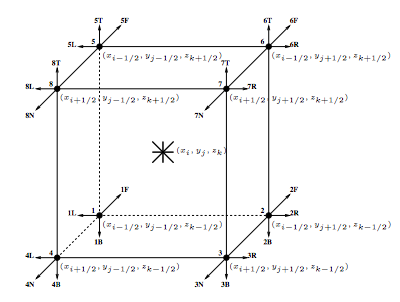
\includegraphics[width=0.6\linewidth]{figures/CartesianDiscretization.jpg}
\caption{Cartesian discretization to be used for the cell balance schemes.}
\label{fig:CartesianDiscretization}
\end{figure}



\subsubsubsection{Cell Balance Schemes}

Cell balance schemes point values for the solution \(\psi\) over a discretized spatial mesh. With the definitions in Eq. \eqref{eq:OmegaComponentsCartesian} switched around to be consistent with the Denovo manual, integrating Eq. \eqref{eq:SimpleTE} over the mesh cell shown in Fig. \ref{fig:CartesianDiscretization} gives:

\begin{equation}
\int_{x_{i-1/2}}^{x_{i+1/2}}dx\mu \frac{\partial \psi}{\partial x}+\int_{y_{j-1/2}}^{y_{j+1/2}}dy\eta \frac{\partial \psi}{\partial y}+\int_{z_{k-1/2}}^{z_{k+1/2}}dz\xi \frac{\partial \psi}{\partial z}+\Sigma_{t,ijk}{E}\psi_{ijk}(\vv{r},E)=S_{ijk}(E)
\end{equation}

where it has been assumed that \(\Sigma_t\) and \(S\) are constant over the cell, and are represented by their cell-centered values. In addition, the energy-dependence has been dropped, though the dependency could easily be re-introduced by simply carrying around the \((E, t)\) notation after each occurrence of \(\psi\). Without approximation, the integrals in the above reduce to:

\begin{equation}
\label{eq:DiscretizedCartesianTE}
\frac{\mu}{\Delta_i}(\psi_{i+1/2}-\psi_{i-1/2})+\frac{\eta}{\Delta_j}(\psi_{j+1/2}-\psi_{j-1/2})+\frac{\xi}{\Delta_k}(\psi_{k+1/2}-\psi_{k-1/2})+\Sigma_{t,ijk}\psi_{ijk}=S_{ijk}
\end{equation}

With this discretization method, there must be some way to relate the cell-centered value \(ijk\) to the face values. The different options we have for discretization are related to the choices we can make for how to relate these quantities. The Diamond Difference and Step Difference schemes choose the following relationship:

\begin{equation}
\label{eq:DifferencingRelationship}
\psi_{i\pm1/2}=\frac{2}{1\pm\alpha}\psi_{ijk}-\frac{1\mp\alpha}{1\pm\alpha}\bar{\psi}_{i\mp1/2}
\end{equation}

and likewise for the \(y\) and \(z\) directions. \(\bar{\psi}\) represents a known flux, and depending on whether a sweep is being performed in the positive-\(\mu\) direction (\(\bar{\psi}_{i-1/2}\) is known) or in the negative-\(\mu\) direction (\(\bar{\psi}_{i+1/2}\) is known), either the + or - option is selected in Eq. \eqref{eq:DifferencingRelationship}. The objective is to choose the correct relationship in Eq. \eqref{eq:DifferencingRelationship} such that the known quantities, or the incoming fluxes to each cell, can be used to compute the unknown quantities, or the outgoing fluxes for each cell, in a ``sweep'' over the spatial mesh. For example, for a sweep in the positive-\(\mu\) direction, we supposedly know \(\bar{\psi}_{i-1/2}\), so we would relate the cell-centered flux to the outgoing flux in the following way:

\begin{equation}
\begin{aligned}
\psi_{i+1/2}=\frac{2}{1+\alpha}\psi_{ijk}-\frac{1-\alpha}{1+\alpha}\bar{\psi}_{i-1/2}\quad\quad\mu >0\\
\psi_{ijk}=\frac{1}{2}\left\lbrack(1+\alpha)\psi_{i+1/2}+(1-\alpha)\bar{\psi}_{i-1/2}\right\rbrack\\
\end{aligned}
\end{equation}

Likewise, for a sweep in the negative-\(\mu\) direction, we supposedly know \(\bar{\psi}_{i+1/2}\), so we would relate the cell-centered flux to the outgoing flux in the following way:

\begin{equation}
\begin{aligned}
\psi_{i-1/2}=\frac{2}{1-\alpha}\psi_{ijk}-\frac{1+\alpha}{1-\alpha}\bar{\psi}_{i+1/2}\quad\quad\mu <0\\
\psi_{ijk}=\frac{1}{2}\left\lbrack(1+\alpha)\psi_{i+1/2}+(1-\alpha)\bar{\psi}_{i-1/2}\right\rbrack\\
\end{aligned}
\end{equation}

Note that both of these provide equivalent expressions, but the choice depends on the sweep direction. The differencing scheme in Eq. \eqref{eq:DifferencingRelationship} is a Crank-Nicolson method in space. Inserting Eq. \eqref{eq:DifferencingRelationship} into the discretized transport equation in Eq. \eqref{eq:SimpleTE} gives the following equation for the cell-centered flux in terms of known quantities:

\begin{equation}
\label{eq:psi_ijk}
\psi_{ijk}=\frac{S_{ijk}+\frac{2}{1\pm\alpha}\left(\frac{|\mu|}{\Delta_i}\bar{\psi}_{i\mp1/2}+\frac{|\eta|}{\Delta_j}\bar{\psi}_{j\mp1/2}\right)+\frac{|\xi|}{\Delta_k}\bar{\psi}_{k\mp1/2}}{\Sigma_{t,ijk}+\frac{2}{1\pm\alpha}\left(\frac{|\mu|}{\Delta_i}+\frac{|\eta|}{\Delta_j}+\frac{|\xi|}{\Delta_k}\right)}
\end{equation}

where it has been assumed that \(\alpha\) is selected to be the same in all directions. \(\alpha\) is a parameter used to tune the spatial discretization. Common choices for \(\alpha\) have their own names. The Diamond Difference method sets \(\alpha=0\). With this choice, the cell-centered flux is an average of the face fluxes. The Step Difference method, on the other hand, sets \(\alpha=\pm1\) such that the cell-centered flux is set equal to the incoming face flux (choose 1 or -1 accordingly so that Eq. \eqref{eq:DifferencingRelationship} provides an expression for \(\psi_{ijk}\) in terms of the known incoming face flux).The Diamond Difference method is second-order in space, while the Step Difference method is only first-order. 

In a ``transport sweep,'' computation begins at a boundary for which the boundary condition is known. At this boundary, the incoming fluxes are known. Then, Eq. \eqref{eq:psi_ijk} is used to solve for \(\psi_{ijk}\) using the incoming flux values. Once the cell-centered flux is known, Eq. \eqref{eq:DifferencingRelationship} can be used to compute the outgoing cell fluxes, which serve as the incoming flux values for the next mesh cell. This process is repeated until each cell has been computed. If there are no scattering, fission, or external sources in Eq. \eqref{eq:psi_ijk}, then only one transport sweep is required. However, if these sources are present, then at the end of each sweep, an updated \(S_{ijk}\) must be computed, and the sweep repeated until reaching convergence. 

If reflective boundary conditions are present, then begin from the side of the domain for which the conditions are known, and then upon reaching the reflective boundary, apply the reflective condition, then perform a sweep in the opposite direction (using the other stepping relations developed for \(\mu<0\) instead of \(\mu>0\)). This double sweep is then halted to perform updates to \(S_{ijk}\) and then repeated until reaching convergence. If reflective boundary conditions exist on both ends of the domain, then an initial guess for the incoming fluxes at the starting point must be made, and then each double sweep is again halted to perform updates to \(S_{ijk}\) until reaching convergence. 

The Diamond Difference method can produce negative fluxes, and the onset of negative fluxes is related to the mesh spacing \(\Delta_i\). 

\begin{tcolorbox}[breakable]
The onset of negative fluxes with the Diamond Difference method can be shown by solving the 1-D, no-source form of Eq. \eqref{eq:SimpleTE} and then applying the Diamond Difference differencing scheme.

\begin{equation}
\label{eq:Ex2}
\mu\frac{d\psi}{dx}+\Sigma_t\psi=0
\end{equation}

The analytical solution to this equation is:

\begin{equation}
\frac{d\psi}{\psi}=\frac{-\Sigma_t}{\mu}dx\quad\rightarrow\quad\int_{x_{i-1/2}}^{x_{i+1/2}}\frac{d\psi}{\psi}=\int_{x_{i-1/2}}^{x_{i+1/2}}\frac{-\Sigma_t}{\mu}dx
\end{equation}

Performing the integration:

\begin{equation}
\label{eq:124}
\ln{\left(\frac{\psi_{i+1/2}}{\psi_{i-1/2}}\right)}=\frac{-\Sigma_t}{\mu}\Delta_i\quad\rightarrow\quad\psi_{i+1/2}=\exp{\left(\frac{-\Sigma_t}{\mu}\Delta_i\right)}\psi_{i-1/2}
\end{equation}

Alternatively, the Diamond Difference method can be used to determine how \(\psi_{i+1/2}\) is related (numerically, instead of analytically) to \(\psi_{i-1/2}\). Using \(\alpha=0\) in Eq. \eqref{eq:DifferencingRelationship}:

\begin{equation}
\label{eq:122}
\psi_{ijk}=\frac{1}{2}\left(\psi_{i+1/2}+\psi_{i-1/2}\right)
\end{equation}

The numeric form of Eq. \eqref{eq:Ex2} can be obtained in a manner very similar to that in Eq. \eqref{eq:DiscretizedCartesianTE}:

\begin{equation}
\label{eq:123}
\frac{\mu}{\Delta_i}(\psi_{i+1/2}-\psi_{i-1/2})+\Sigma_{t,ijk}\psi_{ijk}=0
\end{equation}

Inserting Eq. \eqref{eq:122} into Eq. \eqref{eq:123} to eliminate \(\psi_{ijk}\) in order to obtain an expression similar to that in Eq. \eqref{eq:124} in terms of only \(\psi_{i+1/2}\) and \(\psi_{i-1/2}\):

\begin{equation}
\psi_{i+1/2}=\frac{1-\Sigma_{t,ijk}\Delta_i/2\mu}{1+\Sigma_{t,ijk}\Delta_i/2\mu}\psi_{i-1/2}
\end{equation}

From this expression, \(\psi_{i+1/2}\) can be negative if:

\begin{equation}
\Delta_i>\frac{2|\mu|}{\Sigma_{t,ijk}}
\end{equation}

By comparing this numerical expression with the analytic expression in Eq. \eqref{eq:124}, we see that the truncation error in the Diamond Difference method is that the numerical expression on the LHS below is used to approximate the exponential term on the RHS:

\begin{equation}
\label{eq:125}
\frac{1-\Sigma_{t,ijk}\Delta_i/2\mu}{1+\Sigma_{t,ijk}}\approx\exp{\left(\frac{-\Sigma_t}{\mu}\Delta_i\right)}
\end{equation}

To determine the order of the truncation error, the Taylor series of \(e^x=1+x+\mathscr{O}(x^2)\). So, for the exponential on the RHS, the Taylor series is:

\begin{equation}
\text{Taylor series of } \exp{\left(\frac{-\Sigma_t}{\mu}\Delta_i\right)}=1+\frac{-\Sigma_{t,ijk}}{\mu}\Delta_i+\mathscr{\Delta_i}^2
\end{equation}

The term in the numerator of the fraction on the LHS of Eq. \eqref{eq:125} is very similar to the Taylor series above, and hence we can see that the truncation error of the Diamond Difference method in this case is of \(\mathscr{O}(\Sigma_t\Delta_i/2|\mu|)^2\). 

\end{tcolorbox}

\subsubsection{Quadrature}

\subsubsubsection{Level-Symmetric Quadrature}
While there are many options for quadrature sets, the Level-Symmetric quadrature set is the set most often associated with the \(S_N\) method. With this set, there are \(N(N+2)\) angular directions per spatial location (N(N+2)/8 per octant). The Level-Symmetric quadrature set uses the same set of \(N/2\) positive values of direction cosines for each of the components of \(\hO  \). Because this quadrature set is symmetric, no direction gets preferential treatment. Different quadrature sets could be used for different computations where it is expected for streaming to occur preferentially in some directions over others. 

Because of the symmetry constraints, not all of the choices for the quadrature points are independent, and in fact there is only one degree of freedom for each choice of quadrature set. A second constraint given by Eq. \eqref{eq:QuadratureNormalization} then narrows down the options for the quadrature set. With these two constraints, \(S_2\) quadrature is fixed, but for higher orders, there are several options remaining for the quadrature points. 

\subsubsubsection{\(LQ_N\) Quadrature}

With the same symmetry and normalization constraints as the Level-Symmetric quadrature set, the \(LQ_N\) quadrature set imposes the additional requirement that the quadrature set should correctly integrate as many Legendre polynomials as possible. 

\subsubsection{Spatial Discretization}

The \(S_N\) equations provide the framework to discretize the angular flux in angle, but the equations still must be discretized in space. In general, there are two different means to perform spatial discretization - cell balance methods, which preserve conservation of the solution, and finite element methods, which do not necessarily preserve conservation of the solution. In a single mesh cell, cell balance methods will provide a statement that is equivalent to conservation of neutrons, while finite element methods satisfy the governing equation in a weighted-integral sense. For simplicity, all of the spatial discretization schemes discussed here are applied to the simplified transport equation that neglects time dependence and assumes some angular discretization has already been applied to \(\psi\) such that it is independent of angle (in each of these equations):

\begin{equation}
\label{eq:SimpleTE}
\hO  \cdot\nabla\psi(\vv{r},E)+\Sigma_t({\vv{r},E})\psi(\vv{r},E)=S(\vv{r},E)
\end{equation}

where \(S\) represents the scattering, fission, and external sources. There will be one of these equations for each discrete direction in the \(S_N\) method. For all the following discretization schemes, a Cartesian mesh given in Fig. \ref{fig:CartesianDiscretization} is assumed, with \(i\) representing indices in the \(x\)-direction, \(j\) in the \(y\)-direction, and \(k\) in the \(z\)-direction.

\begin{figure}[H]
\centering
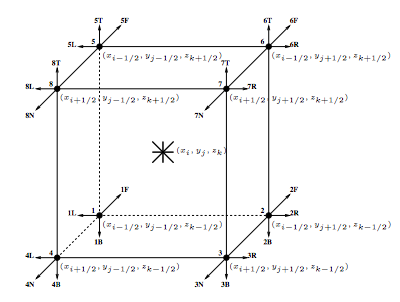
\includegraphics[width=0.6\linewidth]{figures/CartesianDiscretization.jpg}
\caption{Cartesian discretization to be used for the cell balance schemes.}
\label{fig:CartesianDiscretization}
\end{figure}

\subsubsubsection{Cell Balance Schemes}

Cell balance schemes point values for the solution \(\psi\) over a discretized spatial mesh. With the definitions in Eq. \eqref{eq:OmegaComponentsCartesian} switched around to be consistent with the Denovo manual, integrating Eq. \eqref{eq:SimpleTE} over the mesh cell shown in Fig. \ref{fig:CartesianDiscretization} gives:

\begin{equation}
\int_{x_{i-1/2}}^{x_{i+1/2}}dx\mu \frac{\partial \psi}{\partial x}+\int_{y_{j-1/2}}^{y_{j+1/2}}dy\eta \frac{\partial \psi}{\partial y}+\int_{z_{k-1/2}}^{z_{k+1/2}}dz\xi \frac{\partial \psi}{\partial z}+\Sigma_{t,ijk}{E}\psi_{ijk}(\vv{r},E)=S_{ijk}(E)
\end{equation}

where it has been assumed that \(\Sigma_t\) and \(S\) are constant over the cell, and are represented by their cell-centered values. In addition, the energy-dependence has been dropped, though the dependency could easily be re-introduced by simply carrying around the \((E, t)\) notation after each occurrence of \(\psi\). Without approximation, the integrals in the above reduce to:

\begin{equation}
\label{eq:DiscretizedCartesianTE}
\frac{\mu}{\Delta_i}(\psi_{i+1/2}-\psi_{i-1/2})+\frac{\eta}{\Delta_j}(\psi_{j+1/2}-\psi_{j-1/2})+\frac{\xi}{\Delta_k}(\psi_{k+1/2}-\psi_{k-1/2})+\Sigma_{t,ijk}\psi_{ijk}=S_{ijk}
\end{equation}

With this discretization method, there must be some way to relate the cell-centered value \(ijk\) to the face values. The different options we have for discretization are related to the choices we can make for how to relate these quantities. The Diamond Difference and Step Difference schemes choose the following relationship:

\begin{equation}
\label{eq:DifferencingRelationship}
\psi_{i\pm1/2}=\frac{2}{1\pm\alpha}\psi_{ijk}-\frac{1\mp\alpha}{1\pm\alpha}\bar{\psi}_{i\mp1/2}
\end{equation}

and likewise for the \(y\) and \(z\) directions. \(\bar{\psi}\) represents a known flux, and depending on whether a sweep is being performed in the positive-\(\mu\) direction (\(\bar{\psi}_{i-1/2}\) is known) or in the negative-\(\mu\) direction (\(\bar{\psi}_{i+1/2}\) is known), either the + or - option is selected in Eq. \eqref{eq:DifferencingRelationship}. The objective is to choose the correct relationship in Eq. \eqref{eq:DifferencingRelationship} such that the known quantities, or the incoming fluxes to each cell, can be used to compute the unknown quantities, or the outgoing fluxes for each cell, in a ``sweep'' over the spatial mesh. For example, for a sweep in the positive-\(\mu\) direction, we supposedly know \(\bar{\psi}_{i-1/2}\), so we would relate the cell-centered flux to the outgoing flux in the following way:

\begin{equation}
\begin{aligned}
\psi_{i+1/2}=\frac{2}{1+\alpha}\psi_{ijk}-\frac{1-\alpha}{1+\alpha}\bar{\psi}_{i-1/2}\quad\quad\mu >0\\
\psi_{ijk}=\frac{1}{2}\left\lbrack(1+\alpha)\psi_{i+1/2}+(1-\alpha)\bar{\psi}_{i-1/2}\right\rbrack\\
\end{aligned}
\end{equation}

Likewise, for a sweep in the negative-\(\mu\) direction, we supposedly know \(\bar{\psi}_{i+1/2}\), so we would relate the cell-centered flux to the outgoing flux in the following way:

\begin{equation}
\begin{aligned}
\psi_{i-1/2}=\frac{2}{1-\alpha}\psi_{ijk}-\frac{1+\alpha}{1-\alpha}\bar{\psi}_{i+1/2}\quad\quad\mu <0\\
\psi_{ijk}=\frac{1}{2}\left\lbrack(1+\alpha)\psi_{i+1/2}+(1-\alpha)\bar{\psi}_{i-1/2}\right\rbrack\\
\end{aligned}
\end{equation}

Note that both of these provide equivalent expressions, but the choice depends on the sweep direction. The differencing scheme in Eq. \eqref{eq:DifferencingRelationship} is a Crank-Nicolson method in space. Inserting Eq. \eqref{eq:DifferencingRelationship} into the discretized transport equation in Eq. \eqref{eq:SimpleTE} gives the following equation for the cell-centered flux in terms of known quantities:

\begin{equation}
\label{eq:psi_ijk}
\psi_{ijk}=\frac{S_{ijk}+\frac{2}{1\pm\alpha}\left(\frac{|\mu|}{\Delta_i}\bar{\psi}_{i\mp1/2}+\frac{|\eta|}{\Delta_j}\bar{\psi}_{j\mp1/2}+\frac{|\xi|}{\Delta_k}\bar{\psi}_{k\mp1/2}\right)}{\Sigma_{t,ijk}+\frac{2}{1\pm\alpha}\left(\frac{|\mu|}{\Delta_i}+\frac{|\eta|}{\Delta_j}+\frac{|\xi|}{\Delta_k}\right)}
\end{equation}

where it has been assumed that \(\alpha\) is selected to be the same in all directions. \(\alpha\) is a parameter used to tune the spatial discretization. Common choices for \(\alpha\) have their own names. The Diamond Difference method sets \(\alpha=0\). With this choice, the cell-centered flux is an average of the face fluxes. The Step Difference method, on the other hand, sets \(\alpha=\pm1\) such that the cell-centered flux is set equal to the incoming face flux (choose 1 or -1 accordingly so that Eq. \eqref{eq:DifferencingRelationship} provides an expression for \(\psi_{ijk}\) in terms of the known incoming face flux).The Diamond Difference method is second-order in space, while the Step Difference method is only first-order. 

In a ``transport sweep,'' computation begins at a boundary for which the boundary condition is known. At this boundary, the incoming fluxes are known. Then, Eq. \eqref{eq:psi_ijk} is used to solve for \(\psi_{ijk}\) using the incoming flux values. Once the cell-centered flux is known, Eq. \eqref{eq:DifferencingRelationship} can be used to compute the outgoing cell fluxes, which serve as the incoming flux values for the next mesh cell. This process is repeated until each cell has been computed. If there are no scattering, fission, or external sources in Eq. \eqref{eq:psi_ijk}, then only one transport sweep is required. However, if these sources are present, then at the end of each sweep, an updated \(S_{ijk}\) must be computed, and the sweep repeated until reaching convergence. 

If reflective boundary conditions are present, then begin from the side of the domain for which the conditions are known, and then upon reaching the reflective boundary, apply the reflective condition, then perform a sweep in the opposite direction (using the other stepping relations developed for \(\mu<0\) instead of \(\mu>0\)). This double sweep is then halted to perform updates to \(S_{ijk}\) and then repeated until reaching convergence. If reflective boundary conditions exist on both ends of the domain, then an initial guess for the incoming fluxes at the starting point must be made, and then each double sweep is again halted to perform updates to \(S_{ijk}\) until reaching convergence. 

The Diamond Difference method can produce negative fluxes, and the onset of negative fluxes is related to the mesh spacing \(\Delta_i\). Some codes have options called ``Negative-Flux-Fixup'' that remedy these negative fluxes in order to still use relatively coarse spatial meshes. In these methods, whenever an outgoing flux is computed to be negative, then the face flux is set to zero, and \(\psi_{ijk}\) recalculated. This is repeated until all outgoing fluxes are positive. Because the corrected solution depends on \(\psi\), this method is nonlinear.  

\begin{tcolorbox}[breakable]
The onset of negative fluxes with the Diamond Difference method can be shown by solving the 1-D, no-source form of Eq. \eqref{eq:SimpleTE} and then applying the Diamond Difference differencing scheme.

\begin{equation}
\label{eq:Ex2}
\mu\frac{d\psi}{dx}+\Sigma_t\psi=0
\end{equation}

The analytical solution to this equation is:

\begin{equation}
\frac{d\psi}{\psi}=\frac{-\Sigma_t}{\mu}dx\quad\rightarrow\quad\int_{x_{i-1/2}}^{x_{i+1/2}}\frac{d\psi}{\psi}=\int_{x_{i-1/2}}^{x_{i+1/2}}\frac{-\Sigma_t}{\mu}dx
\end{equation}

Performing the integration:

\begin{equation}
\label{eq:124}
\ln{\left(\frac{\psi_{i+1/2}}{\psi_{i-1/2}}\right)}=\frac{-\Sigma_t}{\mu}\Delta_i\quad\rightarrow\quad\psi_{i+1/2}=\exp{\left(\frac{-\Sigma_t}{\mu}\Delta_i\right)}\psi_{i-1/2}
\end{equation}

Alternatively, the Diamond Difference method can be used to determine how \(\psi_{i+1/2}\) is related (numerically, instead of analytically) to \(\psi_{i-1/2}\). Using \(\alpha=0\) in Eq. \eqref{eq:DifferencingRelationship}:

\begin{equation}
\label{eq:122}
\psi_{ijk}=\frac{1}{2}\left(\psi_{i+1/2}+\psi_{i-1/2}\right)
\end{equation}

The numeric form of Eq. \eqref{eq:Ex2} can be obtained in a manner very similar to that in Eq. \eqref{eq:DiscretizedCartesianTE}:

\begin{equation}
\label{eq:123}
\frac{\mu}{\Delta_i}(\psi_{i+1/2}-\psi_{i-1/2})+\Sigma_{t,ijk}\psi_{ijk}=0
\end{equation}

Inserting Eq. \eqref{eq:122} into Eq. \eqref{eq:123} to eliminate \(\psi_{ijk}\) in order to obtain an expression similar to that in Eq. \eqref{eq:124} in terms of only \(\psi_{i+1/2}\) and \(\psi_{i-1/2}\):

\begin{equation}
\psi_{i+1/2}=\frac{1-\Sigma_{t,ijk}\Delta_i/2\mu}{1+\Sigma_{t,ijk}\Delta_i/2\mu}\psi_{i-1/2}
\end{equation}

From this expression, \(\psi_{i+1/2}\) can be negative if:

\begin{equation}
\Delta_i>\frac{2|\mu|}{\Sigma_{t,ijk}}
\end{equation}

By comparing this numerical expression with the analytic expression in Eq. \eqref{eq:124}, we see that the truncation error in the Diamond Difference method is that the numerical expression on the LHS below is used to approximate the exponential term on the RHS:

\begin{equation}
\label{eq:125}
\frac{1-\Sigma_{t,ijk}\Delta_i/2\mu}{1+\Sigma_{t,ijk}}\approx\exp{\left(\frac{-\Sigma_t}{\mu}\Delta_i\right)}
\end{equation}

To determine the order of the truncation error, the Taylor series of \(e^x=1+x+\mathscr{O}(x^2)\). So, for the exponential on the RHS, the Taylor series is:

\begin{equation}
\text{Taylor series of } \exp{\left(\frac{-\Sigma_t}{\mu}\Delta_i\right)}=1+\frac{-\Sigma_{t,ijk}}{\mu}\Delta_i+\mathscr{O}(\Delta_i)^2
\end{equation}

The term in the numerator of the fraction on the LHS of Eq. \eqref{eq:125} is very similar to the Taylor series above, and hence we can see that the truncation error of the Diamond Difference method in this case is of \(\mathscr{O}(\Sigma_t\Delta_i/2|\mu|)^2\). 
\end{tcolorbox}

Aside from the Diamond Difference and Step Difference schemes, a third differencing scheme, Theta-Weighted Diamond Difference, chooses two additional weight parameters based on the incoming fluxes. These additional parameters allow the outgoing fluxes to vary smoothly between the Step and Diamond Difference schemes. These weighting parameters are bounded between the Diamond Difference and Step Difference methods. Provided the source is positive, the Theta-Weighted Diamond Difference and Weighted Diamond Difference with Flux-Fixup both give positive fluxes.

\subsubsection{Operator Form}

This section covers the operator form of the transport equation, where the scattering term has been expanded in spherical harmonics as in Eq. \eqref{eq:SnGeneral}, repeated below for convenience:

\begin{equation}
\label{eq:StartofOperatorForm}
\begin{aligned}
 \hO  _a\cdot\nabla\psi_a^g(\vv{r}) + 
 \Sigma_t^g(\vv{r})\psi_a^g(\vv{r}) = \\
\sum_{l=0}^{N}\left\lbrack Y_{l0}^e(\hO  _a)s_{l0}^g(\vv{r})+\sum_{m=1}^{l}\left(Y_{lm}^e(\hO  _a)s_{lm}^g(\vv{r})+Y_{lm}^o(\hO  _a)v_{lm}^g(\vv{r})\right)\right\rbrack+\\
\sum_{g'=1}^G\sum_{l=0}^{N}\Sigma_{s,l}(\vv{r}, g'\rightarrow g)\left\lbrack Y_{l0}^e(\hO  _a)e_{l0}^{g'}(\vv{r})+\sum_{m=1}^{l}\left(Y_{lm}^e(\hO  _a)e_{lm}^{g'}(\vv{r})+Y_{lm}^o(\hO  _a)o_{lm}^{g'}(\vv{r})\right)\right\rbrack\quad\\
\end{aligned}
\end{equation}

where the equation has now been transformed to a form that accounts for energy groups, rather than applying to a within-group equation. So, all energy dependence is removed, since a group structure now accounts for that dependence. The \(g\) superscript refers to the energy group number, and \(G\) to the total number of energy groups. Within-group scattering is counted in the scattering term, but is canceled by the total interaction term, which avoids double counting. The above equation can be cast in operator form. The external group source is defined as:

\begin{equation}
q_e^g(\vv{r})=\sum_{l=0}^{N}\left\lbrack Y_{l0}^e(\hO  _a)s_{l0}^g(\vv{r})+\sum_{m=1}^{l}\left(Y_{lm}^e(\hO  _a)s_{lm}^g(\vv{r})+Y_{lm}^o(\hO  _a)v_{lm}^g(\vv{r})\right)\right\rbrack
\end{equation}

in order to permit easier equation manipulation. In addition, several operators are defined. The transport operator is:

\begin{equation}
\textbf{L}\equiv\hO  _a\cdot\nabla+\Sigma_t^g
\end{equation}

and the solution vector \(\Psi\) is a column vector containing each energy group flux vector \(\vv{\psi}\):

\begin{equation}
\Psi=\begin{bmatrix}\vv{\psi}_1&\vv{\psi}_2&\vv{\psi}_3&\cdots&\vv{\psi}_G\end{bmatrix}^T
\end{equation}

where \(\vv{\psi}\) is then a column vector that contains the flux for each discrete angle for that particular energy group \(g\):

\begin{equation}
\vv{\psi}_g=\begin{bmatrix}\psi_1^g&\psi_2^g&\psi_3^g&\cdots&\psi_n^g\end{bmatrix}^T
\end{equation}

So, the vector of unknowns is organized by energy group, and in the section pertaining to each group, by angle. In order to discuss the size of these matrices and vectors, several variables are defined:

\begin{equation}
\begin{aligned}
G=&\ \text{number of energy groups}\\
t = &\ \text{number of moments}\\
n = &\ \text{number of angles}\\
N = &\ P_N\text{\ order}\\
N_c=&\ \text{number of cells}\\
N_e=&\ \text{number of unknowns per cell}\\
\end{aligned}
\end{equation} 

So, if the problem consisted of a single cell with a single node (i.e. only one spatial unknown), then \(\Psi\) would be an \((Gn)\times1\) vector. However, the problems solves will consist of a spatial domain that is also present in \(\Psi\). In reality, each \(\psi_{\hO  _n}^g\) term is solved as a function of space, and is therefore not a scalar value, but an \(N_cN_e\times1\) vector. The \(S_N\) equation for a particular angle and group is solved as a function of space using a variety of methods, such as the finite element method or the finite difference method. So, the total size of \(\Psi\) is \(N_cN_eGn\times1\). The external source \(q_e^g\) is defined in a similar manner, and is represented as \(Q\), an \(N_cN_eGn\times1\) vector.

Expressing the mapping between flux moments and the scattering term is more difficult simply due to the difficulty in visualizing the matrix multiplication. The moment-to-discrete matrix is used to project harmonic moments onto discrete angle space. It is defined as:

\begin{equation}
\textbf{M}=\left\{
\begin{array}{*{13}c}
Y_{00}^o(\hO  _1) & Y_{00}^e(\hO  _1) & Y_{01}^o(\hO  _1) & Y_{01}^e(\hO  _1) & Y_{10}^o(\hO  _1) & Y_{10}^e(\hO  _1) & Y_{11}^o(\hO  _1) & Y_{11}^e(\hO  _1) & \cdots & Y_{NN}^o(\hO  _1) & Y_{NN}^e(\hO  _1)\\
Y_{00}^o(\hO  _2) & Y_{00}^e(\hO  _2) & Y_{01}^o(\hO  _2) & Y_{01}^e(\hO  _2) & Y_{10}^o(\hO  _2) & Y_{10}^e(\hO  _2) & Y_{11}^o(\hO  _2) & Y_{11}^e(\hO  _2) & \cdots & Y_{NN}^o(\hO  _2) & Y_{NN}^e(\hO  _2)\\
\vdots & \vdots & \vdots & \vdots & \vdots & \vdots & \vdots & \vdots & \vdots & \vdots & \vdots \\
Y_{00}^o(\hO  _n) & Y_{00}^e(\hO  _n) & Y_{01}^o(\hO  _n) & Y_{01}^e(\hO  _n) & Y_{10}^o(\hO  _n) & Y_{10}^e(\hO  _n) & Y_{11}^o(\hO  _n) & Y_{11}^e(\hO  _n) & \cdots & Y_{NN}^o(\hO  _n) & Y_{NN}^e(\hO  _n)\\
\end{array}\right\}
\end{equation}

But, some of these components are actually always zero - for instance, from the expansion in Eq. \eqref{eq:StartofOperatorForm}, if \(l=0\), then there are no spherical harmonics for which \(m\neq0\). This eliminates \(Y_{01}^e\) and \(Y_{01}^o\). In addition, \(Y_{00}^o=0\) and \(Y_{10}^o=0\) since there is no odd component for \(l=0,i\) and \(m=0\). This gives a simplified version of the moment-to-discrete matrix, where the only difference between this matrix and the more explicit one above is that several of the low \(l\) and \(m\) spherical harmonics that are zero are removed.

\begin{equation}
\textbf{M}=\left\{
\begin{array}{*{13}c}
Y_{00}^e(\hO  _1)  & Y_{10}^e(\hO  _1) & Y_{11}^o(\hO  _1) & Y_{11}^e(\hO  _1) & Y_{20}^e(\hO  _1) & \cdots & Y_{NN}^o(\hO  _1) & Y_{NN}^e(\hO  _1)\\
Y_{00}^e(\hO  _2)  & Y_{10}^e(\hO  _2) & Y_{11}^o(\hO  _2) & Y_{11}^e(\hO  _2) & Y_{20}^e(\hO  _2) & \cdots & Y_{NN}^o(\hO  _2) & Y_{NN}^e(\hO  _2)\\
\vdots & \vdots & \vdots & \vdots & \vdots & \vdots & \vdots & \vdots \\
Y_{00}^e(\hO  _n) & Y_{10}^e(\hO  _n) & Y_{11}^o(\hO  _n) & Y_{11}^e(\hO  _n) & Y_{20}^e(\hO  _n) & \cdots & Y_{NN}^o(\hO  _n) & Y_{NN}^e(\hO  _n)\\
\end{array}\right\}
\end{equation}

The scattering matrix contains along its diagonal the scattering moments:

\begin{equation}
\textbf{S}_{g^{'}\rightarrow g}=\begin{bmatrix}
\Sigma_{s0}
\end{bmatrix}
\end{equation}

With this definition, the discretization of the transport equation leads to the following matrix system:

\begin{equation}
\textbf{L}\begin{bmatrix}\Psi_1\\\Psi_2\\\Psi_3\\\vdots\\\Psi_G\end{bmatrix}=
\begin{bmatrix}
\textbf{M} & 0 & 0 & 0 & 0\\
0 & \textbf{M} & 0 & 0 & 0\\
0 & 0 & \textbf{M} & 0 & 0\\
0 & 0 & 0 & \cdots & 0\\
0 & 0 & 0 & 0 & \textbf{M}\\
\end{bmatrix}
\begin{bmatrix}
\textbf{S}_{11} & \textbf{S}_{12} & \textbf{S}_{13} & \cdots & \textbf{S}_{1G}\\
\textbf{S}_{21} & \textbf{S}_{22} & \textbf{S}_{23} & \cdots & \textbf{S}_{2G}\\
\textbf{S}_{31} & \textbf{S}_{32} & \textbf{S}_{33} & \cdots & \textbf{S}_{3G}\\
\vdots & \vdots & \vdots & \vdots & \vdots\\
\textbf{S}_{G1} & \textbf{S}_{G2} & \textbf{G}_{23} & \cdots & \textbf{S}_{GG}\\
\end{bmatrix}
\begin{bmatrix}
\Phi_1\\\Phi_2\\\Phi_3\\\vdots\\\Phi_G
\end{bmatrix}
+
\begin{bmatrix}
Q_1\\Q_2\\Q_3\\\vdots\\Q_G
\end{bmatrix}
\end{equation}

Hence, the upper triangular portion of the scattering matrix represents upscattering, while the diagonal represents within-group scattering, and the lower triangular portion represents downscattering. \(\Phi\) represents a vector of the angular flux moments used in the expansion of the scattering term, organized by group. 

\begin{equation}
\Phi_g=\begin{bmatrix}
o_{00}^g & e_{00}^g & o_{01}^g & e_{01}^g & o_{10}^g & e_{10}^g & \cdots & o_{NN}^g & e_{NN}^g\\
\end{bmatrix}^T
\end{equation}

where \(e_{lm}\) and \(o_{lm}\) are defined by Eq. \eqref{eq:FluxMoments31}. Note, however, that some of these terms are zero due to how the expansion is performed. Moments with \(l=0\) are only nonzero for \(m=0\). And, there is no odd component for \(l=0\). 

\begin{equation}
\Phi_g=\begin{bmatrix}
e_{00}^g & e_{10}^g & o_{11}^g & e_{11}^g & \cdots & o_{NN}^g & e_{NN}^g\\
\end{bmatrix}^T
\end{equation}

The flux moment vector can be related to the angular flux vector by \(\textbf{D}\):

\clearpage
\section{The Spectral Angular Method}
\label{sec:PN}

An alternative angular discretization strategy to the discrete ordinates equations described in Section \ref{sec:SN} is to expand the angular dependence of the angular flux in a finite series of orthogonal functions. In general 3-D geometries, these functions are typically selected as the spherical harmonics functions described in Section \ref{sec:SH}. The spherical harmonics functions reduce to the Legendre polynomials in 1-D, so for 1-D geometries, these functions are typically selected as the Legendre polynomials described in Section \ref{sec:LegendrePolynomials}. After the flux has been expanded as a finite sum of functions and inserted into the \gls{nte}, the entire equation is multiplied by a function of different order and properties of orthogonality used to derived a set of coupled equations for the coefficients of the expansion. While the discrete ordinates method requires interpolation between the allowable directions of motion \(\hO_n\), the \(P_N\) method yields a continuous angular dependence.

Expanding the angular flux as a finite series of orthogonal functions is known as the \(P_N\) method. This method provides reasonably-correct spatial solutions, but errors are often present in magnitude that can be difficult to detect.



\clearpage
 
\subsubsection{1-D Cartesian Derivation}

Due to the added complexity associated with higher dimensions, the \(P_N\) equations are derived here for the time-independent form of the 1-D, monoenergetic transport equation in Cartesian geometries given by Eq. \eqref{eq:TE_Cartesian_1D_2_noenergy}, repeated here for reference, where the external and fission source are bundled together into \(S\), which is assumed isotropic:

\begin{equation*}
\mu \frac{\partial \psi(z, \mu)}{\partial z} +
 \Sigma_t(z)\psi(z, \mu) =\int_{4\pi}^{} d\hO  ' \Sigma_s(z, \hO  \cdot\hO  ')\psi(z,\hO  ') + \frac{S(z)}{4\pi}
 \end{equation*}

The \(P_N\) approximation is made by expanding both the flux and scattering cross section in Legendre polynomials in a similar fashion to the scattering cross section as shown in Eq. \eqref{eq:ScatteringLegendre}. We use Legendre polynomials here because we're in 1-D Cartesian geometry; in higher dimensions or in non-Cartesian frames, the spherical harmonics would be needed.

\begin{equation}
\label{eq:AngularFluxPN}
\psi(z,\mu)=\sum_{n=0}^{\infty}\frac{2n+1}{4\pi}\phi_n(z)P_n(\mu)
\end{equation}

\begin{equation}
\label{eq:PNScatteringCrossSectionExpansion}
\Sigma_s(z,\hO  \cdot\hO  ')=\sum_{l=0}^{\infty}\frac{2l+1}{4\pi}\Sigma_{sl}(z)P_l(\hO  \cdot\hO  ')\rightarrow\sum_{l=0}^{\infty}\frac{2l+1}{4\pi}\Sigma_{sl}(z)P_l(\mu)P_l(\mu')
\end{equation}

where \(n\) is used in the expansion of the flux to differentiate it from \(l\) used in expanding the scattering cross section. From the 1-D form of the addition theorem for spherical harmonics given in Eq. \eqref{eq:AddSpherical1D}, the scattering cross section expansion has been simplified. Now, inserting Eqs. \eqref{eq:AngularFluxPN} and \eqref{eq:AngularFluxPN} into the 1-D transport equation listed in the beginning of this section:

\begin{equation}
\begin{aligned}
\mu \frac{\partial}{\partial z}\left(\sum_{n=0}^{\infty}\frac{2n+1}{4\pi}\phi_n(z)P_n(\mu)\right) + \Sigma_t(z)\sum_{n=0}^{\infty}\frac{2n+1}{4\pi}\phi_n(z)P_n(\mu) =\quad\quad\\
\int_{4\pi}^{} d\hO  ' \sum_{l=0}^{\infty}\frac{2l+1}{4\pi}\Sigma_{sl}(z)P_l(\mu)P_l(\mu')\sum_{n=0}^{\infty}\frac{2n+1}{4\pi}\phi_n(z)P_n(\mu) + \frac{S(z)}{4\pi}
 \end{aligned}
 \end{equation}

Because no quantities depend on \(\hO  \), the scattering integral can be integrated over \(0\leq\phi\leq2\pi\) so that the integral becomes a function of only \(\mu\) and space.

\begin{equation}
\label{eq:PNStep1}
\begin{aligned}
\mu \frac{\partial}{\partial z}\left(\sum_{n=0}^{\infty}\frac{2n+1}{4\pi}\phi_n(z)P_n(\mu)\right) + \Sigma_t(z)\sum_{n=0}^{\infty}\frac{2n+1}{4\pi}\phi_n(z)P_n(\mu) =\quad\quad\\
2\pi\int_{-1}^{1} d\mu' \sum_{l=0}^{\infty}\frac{2l+1}{4\pi}\Sigma_{sl}(z)P_l(\mu)P_l(\mu')\sum_{n=0}^{\infty}\frac{2n+1}{4\pi}\phi_n(z)P_n(\mu) + \frac{S(z)}{4\pi}
 \end{aligned}
 \end{equation}
 
The orthogonality property of Legendre polynomials given in Eq. \eqref{eqn:LegendrePolynomialsOrthogonality} does not permit any extra terms (that depend on \(\mu\)) to be present in the integrand. Hence, the first term in Eq. \eqref{eq:PNStep1} must be rewritten using the recursive property of Legendre polynomials given in Eq. \eqref{eqn:LegendrePolynomialRecursion1}:

 \begin{equation}
\label{eq:PNStep2}
\begin{aligned}
\frac{\partial}{\partial z}\left(\sum_{n=0}^{\infty}\frac{\cancel{2n+1}}{4\pi}\phi_n(z)\frac{1}{\cancel{2n+1}} \left\lbrack(n+1)P_{n+1}(\mu) + n P_{n-1}(\mu)\right\rbrack\right) + \Sigma_t(z)\sum_{n=0}^{\infty}\frac{2n+1}{4\pi}\phi_n(z)P_n(\mu) =\quad\quad\\
2\pi\int_{-1}^{1} d\mu' \sum_{l=0}^{\infty}\frac{2l+1}{4\pi}\Sigma_{sl}(z)P_l(\mu)P_l(\mu')\sum_{n=0}^{\infty}\frac{2n+1}{4\pi}\phi_n(z)P_n(\mu) + \frac{S(z)}{4\pi}
 \end{aligned}
 \end{equation}
 
 Multiplying Eq. \eqref{eq:PNStep2} by \(P_n(\mu)\) and then integrating over \(-1\leq\mu\leq1\) gives, after canceling the \(1/4\pi\) from each term:
 
  \begin{equation}
\label{eq:PNStep3}
\begin{aligned}
\frac{\partial}{\partial z}\left(\sum_{n=0}^{\infty}\left\lbrack\int_{-1}^{1}d\mu\phi_n(z)(n+1)P_{n+1}(\mu)P_n(\mu) + \int_{-1}^{1}d\mu\phi_n(z)n P_{n-1}(\mu)P_n(\mu)\right\rbrack\right) + \quad\quad\\
\Sigma_t(z)\sum_{n=0}^{\infty}(2n+1)\int_{-1}^{1}d\mu\phi_n(z)P_n(\mu)P_n(\mu) =\quad\quad\\
\int_{-1}^{1}d\mu P_n(\mu)2\pi\int_{-1}^{1} d\mu' \sum_{l=0}^{\infty}\frac{2l+1}{4\pi}\Sigma_{sl}(z)P_l(\mu)P_l(\mu')\sum_{n=0}^{\infty}(2n+1)\phi_n(z)P_n(\mu)P_n(\mu) + \int_{-1}^{1}d\mu S(z)P_n(\mu)
 \end{aligned}
 \end{equation}

Then, applying the orthogonality property of Legendre polynomials from Eq. \eqref{eqn:LegendrePolynomialsOrthogonality} gives:

  \begin{equation}
\label{eq:PNStep4}
\begin{aligned}
\frac{\partial}{\partial z}\left(\sum_{n=0}^{\infty}\left\lbrack\frac{2(n+1)}{2n+1}\phi_{n+1}(z) +\frac{2n}{2n+1} \phi_{n-1}(z)\right\rbrack\right) + \Sigma_t(z)\sum_{n=0}^{\infty}2\phi_n(z) =\quad\quad\\
2\sum_{l=0}^{\infty}\Sigma_{sl}(z)\sum_{n=0}^{\infty}\phi_n(z) + \int_{-1}^{1}d\mu S(z)P_n(\mu)
 \end{aligned}
 \end{equation}

where orthogonality was applied twice to the scattering term. Dividing through by 2 then gives the \(P_N\) equations for 1-D Cartesian geometries:

\begin{equation}
\label{eq:PNStep5}
\begin{aligned}
\frac{\partial}{\partial z}\left(\sum_{n=0}^{\infty}\left\lbrack\frac{n+1}{2n+1}\phi_{n+1}(z) +\frac{n}{2n+1} \phi_{n-1}(z)\right\rbrack\right) + \Sigma_t(z)\sum_{n=0}^{\infty}\phi_n(z) =\quad\quad\\
\sum_{l=0}^{\infty}\Sigma_{sl}(z)\sum_{n=0}^{\infty}\phi_n(z) + \delta_{n,even}\frac{1}{2}\int_{-1}^{1}d\mu S(z)P_n(\mu)
 \end{aligned}
 \end{equation}

Because \(S(z)\) is not a function of \(\mu\), then the integral of a Legendre polynomial over its basis will give zero if that Legendre polynomial is an odd function, and will be nonzero otherwise. Hence, the source term is only present for even \(n\), based on the first few Legendre polynomials shown in Eq. \eqref{eqn:LegendrePolynomials_P0P1P2}. Now, in order to make this solution method tractable, the infinite sums have to be truncated at some point. It is also customary to set \(l=n\) such that the above reduce to:

\begin{equation}
\label{eq:PNStep6}
\begin{aligned}
\frac{\partial}{\partial z}\left(\sum_{n=0}^{N}\left\lbrack\frac{n+1}{2n+1}\phi_{n+1}(z) +\frac{n}{2n+1} \phi_{n-1}(z)\right\rbrack\right) + \Sigma_t(z)\sum_{n=0}^{N}\phi_n(z) =\quad\quad\\
\sum_{n=0}^{N}\Sigma_{sn}(z)\phi_n(z) +  \delta_{n,even}\frac{1}{2}\int_{-1}^{1}d\mu S(z)P_n(\mu)
 \end{aligned}
 \end{equation}

We can require Eq. \eqref{eq:PNStep6} to hold for all \(N\) at once, but we can also require it to hold for each \(N\). This stricter requirement returns the requirement stated in Eq. \eqref{eq:PNStep6}, and hence the \(P_N\) equations in practice produce \(N\) coupled ODEs:

\begin{equation}
\label{eq:PNEquations}
\begin{aligned}
\frac{\partial}{\partial z}\left\lbrack\frac{n+1}{2n+1}\phi_{n+1}(z) +\frac{n}{2n+1} \phi_{n-1}(z)\right\rbrack + \Sigma_t(z)\phi_n(z) =
\Sigma_{sn}(z)\phi_n(z) +  \delta_{n,even}\frac{1}{2}\int_{-1}^{1}d\mu S(z)P_n(\mu)
 \end{aligned}
 \end{equation}

This gives \(N+1\) coupled equations. For example, some of the first \(P_N\) equations are:
 
 \begin{equation}
 \begin{aligned}
\frac{\partial\phi_{1}(z)}{\partial z} + \Sigma_t(z)\phi_0(z)=\Sigma_{s0}\phi_0(z)+ S_0(z)\quad\quad n=0\\
\frac{2}{3}\frac{\partial\phi_{2}(z)}{\partial z}+\frac{1}{3}\frac{\partial\phi_{0}(z)}{\partial z} + \Sigma_t(z)\phi_1(z)=\Sigma_{s1}\phi_1(z)\quad\quad n=1\\
\frac{3}{5}\frac{\partial\phi_{3}(z)}{\partial z}+\frac{2}{5}\frac{\partial\phi_{1}(z)}{\partial z} + \Sigma_t(z)\phi_2(z)=\Sigma_{s2}\phi_2(z)+ S_2(z)\quad\quad n=2\\
\end{aligned}
\end{equation}

In order to truncate the infinite series to \(N\) unknowns, \(\phi_{-1}=0\) is often set, and either \(\phi_{N+1}=0\) or \(\partial\phi_{N+1}/\partial z=0\) is set as the other condition, where both give equivalent results. \(N\) is usually selected to be odd. If \(N\) were even, then artificial symmetry would be introduced into the problem through application of boundary conditions. In addition, for even \(N\), you do not obtain any additional information (non-linearly independent) from the \(P_N\) equations. 

\subsubsubsection{Boundary Conditions}
Marshak boundary conditions require continuity in the odd flux moments at boundaries. 

\begin{equation}
2\pi\int_{\hO  \cdot\hat{n}<0}^{}d\mu P_l(\mu)\psi(\mu)=2\mu\int_{\hO  \cdot\hat{n}<0}^{}d\mu P_l(\mu)\psi_b(\mu)\quad\quad l=1, 3, 5\cdots N
\end{equation}

where \(\psi_b(\mu)\) is the incoming flux. Expanding flux according to Eq. \eqref{eq:AngularFluxPN} gives:

\begin{equation}
2\pi\int_{\hO  \cdot\hat{n}<0}^{}d\mu P_l(\mu)\sum_{n=0}^{\infty}\frac{2n+1}{4\pi}\phi_n(z)P_n(\mu)=2\mu\int_{\hO  \cdot\hat{n}<0}^{}d\mu P_l(\mu)\psi_b(\mu)\quad\quad l=1, 3, 5\cdots N
\end{equation}

This gives \((N+1)/2\) boundary conditions. For an isotropic boundary:

\begin{equation}
\psi_b(\mu)=\frac{\phi_b}{4\pi}
\end{equation}

For a reflecting boundary, the net current at that boundary is zero. From the form of Eq. \eqref{eq:ScatteringMomentsLegendre}, it can be seen that the flux moments are given by:

\begin{equation}
\phi_l(z)=2\pi\int_{-1}^{1}d\mu\psi(\mu)P_l(\mu)
\end{equation}

For \(l=1\), we see that \(\phi_1\) represents the current. Hence, reflecting boundary conditions extend this argument to require that on vacuum boundaries:

\begin{equation}
\phi_l=0\quad\quad l=1, 3, 5, \cdots, N
\end{equation}

\subsection{Simplified Spherical Harmonics \(SP_N\)}
\label{sec:SPN}

The \(SP_N\), or Simplified \(P_N\), method was developed by Ely Gelbard in the early 1960s as an extension of the 1-D Cartesian \(P_N\) equations to higher dimensions. The \(SP_N\) method represents a``middle-ground'' between the full transport equation and diffusion theory. Gelbard ``derived'' the \(SP_N\) equations by extending the 1-D \(P_N\) equations to 3-D, with relatively little mathematical basis. The \(SP_N\) equations are equivalent to the \(P_N\) equations in slab geometries and in other limited cases, and it is only the relatively good numerical results that justified the use of the method initially, since it was not derived in a particularly rigorous manner. It was not until the 1990s that several mathematicians demonstrated that the \(SP_N\) method does have mathematical foundation, and it was shown that the \(SP_N\) equations are an asymptotic approximation to the transport equation. 

The \(SP_N\) method does not always give superior results to diffusion theory, and if the system is not diffusive or not locally 1-D, then the method gives poorer answers than diffusion theory. Away from the asymptotic limit to the transport equation, the \(SP_N\) equations break down. 

However, the \(SP_N\) equations contain more transport physics than the diffusion equation, and hence can be used to capture boundary layers that would be missed by diffusion theory. With the \(P_N\) equations, in the limit of \(N\rightarrow\infty\), the \(P_N\) solutions converge to the true solution, while this is not necessarily the case with the \(SP_N\) equations. Because the \(SP_N\) equations require higher computational cost, the best intermediate choice is to use the \(SP_3\) equations, since these offer much better solutions than the diffusion equation, without exceptionally higher cost.

A heuristic derivation of the \(SP_N\) equations can be performed using simple arguments regarding the form of the 1-D \(P_N\) equations in Eq. \eqref{eq:PNEquations}. The key to deriving the \(SP_N\) equations is to transform Eq. \eqref{eq:PNEquations} such that the derivative in the even-\(n\) equations is replaced by a divergence, while the derivative in the odd-\(n\) equations is replaced by a gradient. The \(SP_N\) equations therefore are:

\begin{equation}
\label{eq:SPNEquations}
\begin{aligned}
\frac{n+1}{2n+1}\nabla\cdot\vv{\phi}_{n+1}(z)+\frac{n}{2n+1}\nabla\cdot\vv{\phi}_{n-1}(z)+ \Sigma_t(z)\phi_n(z)=\Sigma_{sn}\phi_n(z)+ S_n(z)\quad \textrm{even - } n\\
\frac{n+1}{2n+1}\nabla\phi_{n+1}(z)+\frac{n}{2n+1}\nabla\phi_{n-1}(z)+ \Sigma_t(z)\vv{\phi}_n(z)=\Sigma_{sn}\vv{\phi}_n(z)\quad \textrm{odd - } n\\
\end{aligned}
 \end{equation}

This first-order form gives \(N+1\) equations. The \(SP_N\) equations can also be written in second-order form by solving for the odd moments in the odd-\(n\) equations, and then substituting this into the even moment equations. From the odd-\(n\) equation in Eq. \eqref{eq:SPNEquations}, we obtain:

\begin{equation}
\vv{\phi}_n(z)=\frac{1}{\Sigma_t(z)-\Sigma_{sn}(z)}\left(\frac{n+1}{2n+1}\nabla\phi_{n+1}(z)+\frac{n}{2n+1}\nabla\phi_{n-1}(z)\right)
\end{equation}

because \(\phi_{n+1}\) and \(\phi_n-1\) appear in the \(SP_N\) equations, the above can be used to determine the following additional relationships:

\begin{equation}
\begin{aligned}
\vv{\phi}_{n-1}(z)=\frac{1}{\Sigma_t(z)-\Sigma_{s,n-1}(z)}\left(\frac{n}{2n-1}\nabla\phi_{n}(z)+\frac{n-1}{2n-1}\nabla\phi_{n-2}(z)\right)\\
\vv{\phi}_{n+1}(z)=\frac{1}{\Sigma_t(z)-\Sigma_{s,n+1}(z)}\left(\frac{n+2}{2n+3}\nabla\phi_{n+2}(z)+\frac{n+1}{2n+3}\nabla\phi_{n}(z)\right)\\
\end{aligned}
\end{equation}

Inserting these expressions into the first-order form of the \(SP_N\) equations Eq. \eqref{eq:SPNEquations} then gives the second-order form, which holds for even \(n\):

\begin{equation}
\label{eq:SPNEquations}
\begin{aligned}
\frac{n+1}{2n+1}\nabla\cdot\left\lbrack\frac{1}{\Sigma_t(z)-\Sigma_{s,n+1}(z)}\left(\frac{n+2}{2n+3}\nabla\phi_{n+2}(z)+\frac{n+1}{2n+3}\nabla\phi_{n}(z)\right)\right\rbrack+\quad\quad\\
\frac{n}{2n+1}\nabla\cdot\left\lbrack\frac{1}{\Sigma_t(z)-\Sigma_{s,n-1}(z)}\left(\frac{n}{2n-1}\nabla\phi_{n}(z)+\frac{n-1}{2n-1}\nabla\phi_{n-2}(z)\right)\right\rbrack+\quad\quad\\
 (\Sigma_t(z)-\Sigma_{sn})\phi_n(z)= S_n(z)\\
\end{aligned}
 \end{equation}

The second-order form of the \(SP_N\) equations results in the need to solve half as many equations as the first-order form. In addition, the diffusive behavior of the \(SP_N\) equations makes them much more amenable to solution than the hyperbolic \(P_N\) equations. 

\subsubsection{Boundary Conditions}

Heuristic arguments can be used to determine how the 1-D boundary conditions for the \(P_N\) method can be extended to the \(SP_N\) method. All derivatives are transformed according to \(\partial(.)/\partial x\rightarrow\hat{n}\cdot\nabla(.)\). 

\clearpage
\section{The Diffusion Equation}
\label{sec:Diffusion}

The diffusion equation is a version of the \gls{nte} that is derived by making some simplifying assumptions regarding the angular dependence of the angular flux. Before we reach this conclusion, however, we should explore two possible methods in which we might obtain a \gls{pde} strictly in terms of the scalar flux \(\phi\) and scalar current \(\vv{J}\), defined as:

\beq
\label{eq:ScalarFluxDef}
\phi\sset\equiv\int_{4\pi}d\hO\psi\seat
\eeq

\beq
\label{eq:Current}
\vv{J}(\vv{r},E,t)\equiv\int_{4\pi}^{}d\hO  \vv{j}\seat
\eeq

Our first attempt to obtain an equation solely in terms of \(\phi\) will be to integrate the \gls{nte} in Eq. \eqref{eq:nte1} over angle, using the definitions of scalar flux and current in Eqs. \eqref{eq:ScalarFluxDef} and \eqref{eq:Current}:

\beqa
\label{eq:NeutronContinuityEquation}
&\frac{\partial}{\partial t}\left(\frac{\phi\sset}{v(E)}\right)+\nabla\cdot\vv{J}\sset+\Sigma_t\sset\phi\sset=\\
&\hspace{1cm}\int_{4\pi}d\hO\inscatteringsource\psi\seatelse+\\
&\hspace{2cm}\int_{4\pi}d\hO\chi_p(E,\hO)\dEprime\left\lbrack1-\beta(E')\right\rbrack\nu(E')\Sigma_f(\vv{r},E',t)\phi(\vv{r},E',t)+\\
&\hspace{3cm}\int_{4\pi}d\hO\delayedfissionsource+S\sset
\eeqa

The time term is obtained by expanding via the chain rule, integrating in angle (by noting that the time derivative in the \(\partial/\partial t\) operator can be brought outside the integral due to its lack of dependence on angle, and then brought back in after introducing \(\phi\)), and collapsing the chain rule. The streaming term was written as an area integral by reversing the divergence rule, and then re-applying the divergence rule after angle integration. The fission and total cross sections have been assumed independent of angle such that they could be brought outside the angle integration, as is commonplace. 

The inscattering source term requires additional effort to switch the order of integration of \(\hO'\) and \(\hO\). By assuming rotational symmetry such that Eq. \eqref{eq:OmegaDotOmega} holds, the single differential scattering cross section is defined by integrating over \(\hO\):

\beqa
\label{eq:SingleDifferentialSigma_s}
\Sigma_s(\vv{r},E'\rightarrow E,t)\equiv&\int_{4\pi}d\hO \Sigma_s\seatout\\
=&\ 2\pi\int_{-1}^1d\mu\Sigma_s(E'\rightarrow E,\mu)
\eeqa

Switching the order of angle integrations in the in-scattering term and inserting the definition in Eq. \eqref{eq:SingleDifferentialSigma_s} gives:

\beqa
\label{eq:NeutronContinuityEquation1}
&\frac{\partial}{\partial t}\left(\frac{\phi\sset}{v(E)}\right)+\nabla\cdot\vv{J}\sset+\Sigma_t\sset\phi\sset=\\
&\hspace{1cm}\dEprime\Sigma_s(\vv{r},E'\rightarrow E,t)\phi(\vv{r},E',t)+\\
&\hspace{2cm}\int_{4\pi}d\hO\chi_p(E,\hO)\dEprime\left\lbrack1-\beta(E')\right\rbrack\nu(E')\Sigma_f(\vv{r},E',t)\phi(\vv{r},E',t)+\\
&\hspace{3cm}\int_{4\pi}d\hO\delayedfissionsource+S\sset
\eeqa

Eq. \eqref{eq:NeutronContinuityEquation1} is sometimes referred to as the ``neutron continuity'' equation, since it represents an equivalent statement of neutron conservation, similar to mass conservation in fluid mechanics and the ``mass continuity'' equation. Note that attempting to integrate out all angular dependence has introduced \(\vv{J}\), which has no exact relationship with \(\phi\). We will seek a \gls{pde} that is a function of strictly \(\vv{J}\), rather than both \(\vv{J}\) and \(\phi\), by multiplying the \gls{nte} by \(\hO\) and then integrating in angle. Because \(\hO\) is a vector, this corresponds to the multiplication of the \gls{nte} by each component of \(\hO\) and summing. 

\beqa
\label{eq:TEAngleAngleIntegrated2}
&\frac{\partial}{\partial t}\left(\frac{\vv{J}\sset}{v(E)}\right)+\nabla\cdot\int_{4\pi}d\hO\psi\seat\hO\hO+\Sigma_t\sset\vv{J}\sset=\\
&\hspace{1cm}\int_{4\pi}d\hO\inscatteringsource\psi(\vv{r},E',\hO',t)\hO\ +\\
&\hspace{2cm}\int_{4\pi}d\hO\chi_p(E,\hO)\hO\dEprime \left\lbrack1-\beta(E')\right\rbrack\nu(E')\Sigma_f(\vv{r},E',t)\phi(\vv{r},E',t)\ +\\
&\hspace{3cm}\int_{4\pi}d\hO\hO\delayedfissionsource+\int_{4\pi}d\hO S\seat\hO
\eeqa

The time term is obtained by expanding via the chain rule, integrating in angle (by noting that the time derivative in the \(\partial/\partial t\) operator can be brought outside the integral due to its lack of dependence on angle, and then brought back in after introducing \(\phi\)), and collapsing the chain rule. The gradient is brought outside the angular integral in the streaming term because the operator is independent of angle. Again, the total and fission cross sections are assumed independent of angle such that they can be brought outside the angle integration, with the definition of scalar flux in Eq. \eqref{eq:ScalarFluxDef} used in the fission source term. If the prompt and/or delayed fission spectra are isotropic, then the first moments of \(\chi_p\) and \(\chi_d\) are zero, and the fission source terms are zero. Likewise, the external source integral represents the first moment of the external source, which will be zero if the external source is isotropic.

The inscattering source term again requires some additional effort and tracking of the multiplication by each component of \(\hO\). The \(x\)-component multiplication, with the angle order of integration swapped, reads as:

\beq
\label{eq:Inscat1}
\int_{4\pi}d\hO'\dEprime \int_{4\pi}d\hO\Sigma_s\seatout\psi\seatelse\Omega_x
\eeq

Because \(\hO\) and \(\hO'\) are unit vectors, Eq. \eqref{eq:Inscat1} can be multiplied by \(\hO'\cdot\hO'\equiv1\):

\beq
\label{sec:Inscat1}
\int_{4\pi}d\hO'\dEprime \int_{4\pi}d\hO\Sigma_s\seatout\psi\seatelse\Omega_x\hO'\cdot\hO'
\eeq

Assuming rotational symmetry such that \(\Sigma_s\) depends on \(\hO\cdot\hO'\) rather than the initial and final angle states individually, we express \(\Sigma_s\) in terms of \(\mu\) and write \(\hO'\cdot\hO'\) as \(\Omega'_i\Omega'_i\), where \(i=x\), \(y\), and \(z\), which can be written solely in terms of the \(x\)-component by including an extra factor of 3:

\beq
\label{sec:Inscat2}
3\int_{4\pi}d\hO'\dEprime \int_{4\pi}d\hO\Sigma_s(\vv{r},E'\rightarrow E,\hO'\cdot\hO,t)\psi\seatelse\Omega_x\Omega'_x\Omega'_x
\eeq

Now, by recognizing that the dot product between directions of motion can be reversed from \(\hO'\cdot\hO'\) to \(\hO'\cdot\hO\) gives the following:

\beq
\label{eq:Inscat2}
\dEprime \Sigma_{s,1}(\vv{r},E'\rightarrow E,t)\vv{J}(\vv{r},E',t)
\eeq

where the definition of current from Eq. \eqref{eq:Current} has been used and the first moment of the scattering cross section is defined as:

\beq
\Sigma_{s,1}(\vv{r},E'\rightarrow E,t)\equiv 2\pi\int_{-1}^1d\mu\Sigma_s(\vv{r},E'\rightarrow E,\mu,t)\mu 
\eeq

Combining Eq. \eqref{eq:TEAngleAngleIntegrated2} with the form of the in-scattering source in Eq. \eqref{eq:Inscat2} gives:

\beqa
\label{eq:TEAngleAngleIntegrated2v2}
&\frac{\partial}{\partial t}\left(\frac{\vv{J}\sset}{v(E)}\right)+\nabla\cdot\int_{4\pi}d\hO\psi\seat\hO\hO+\Sigma_t\sset\vv{J}\sset=\\
&\hspace{1cm}\dEprime \Sigma_{s,1}(\vv{r},E'\rightarrow E,t)\vv{J}(\vv{r},E',t)+\\
&\hspace{2cm}\int_{4\pi}d\hO\chi_p(E,\hO)\hO\dEprime \left\lbrack1-\beta(E')\right\rbrack\nu(E')\Sigma_f(\vv{r},E',t)\phi(\vv{r},E',t)+\\
&\hspace{3cm}\int_{4\pi}d\hO\hO\delayedfissionsource+\int_{4\pi}d\hO S\seat\hO
\eeqa

As can be seen in Eq. \eqref{eq:TEAngleAngleIntegrated2v2}, attempting to obtain an equation solely in terms of \(\vv{J}\) has been unsuccessful due to the streaming term. Because the streaming term is the only term that contains a factor of \(\hO\), each multiplication by \(\hO\) and integration over angle will introduce a new term that we cannot express analytically in terms of \(\vv{J}\) or \(\phi\). So, the diffusion equation cannot be derived by simply integrating angular dependence from the \gls{nte} or by performing other tricks like first multiplying by \(\hO\) and then integrating over angle. 

At this point, it is clear that a simpler version of the \gls{nte} in terms of solely \(\phi\) or \(\vv{J}\) cannot be derived, and a more explicit assumption regarding the angular dependence of the angular flux must be made. The diffusion equation is derived from the angle-integrated \gls{nte} in Eq. \eqref{eq:NeutronContinuityEquation1} by assuming a \(P_1\) expansion for the angular dependence of the angular flux according to the form in Eq. \eqref{eq:ScatteringLegendre}:

\beqa
\label{eq:FluxLegendreP1}
\psi\seat\approx&\sum_{l=0}^1\frac{2l+1}{4\pi}\psi_l\sset P_l(\hO)\\
=&\frac{1}{4\pi}\psi_0\sset+\frac{3}{4\pi}\psi_1\sset\hO\\
\eeqa
%\frac{1}{4\pi}\phi\sset+\frac{3}{4\pi}\vv{J}\sset\hO

where \(\psi_l\) is the \(l\)-th moment of the angular flux. Based on the definitions of the first few Legendre polynomials in Eq. \eqref{eqn:LegendrePolynomials_P0P1P2}, a \(P_1\) approximation is equivalent to assuming linear anisotropy in the angular flux. Using a linear approximation for anisotropy is reasonably accurate if the angular flux is only weakly dependent on angle. To interpret the physical meaning of the flux moments \(\psi_0\) and \(\psi_1\), integrate Eq. \eqref{eq:FluxLegendreP1} over angle:

\beqa
\label{eq:FluxLegendreP1_AngleIntegration}
\int_{4\pi}^{} d\hO\psi\seat=& \frac{1}{4\pi}\int_{4\pi}^{}d\hO\psi_0\sset +\frac{3}{4\pi}\int_{4\pi}^{} d\hO \psi_1\sset\hO\\
\phi\spas = &\ \psi_0 + \frac{3}{4\pi}\psi_1\int_{4\pi}^{} d\hO  \hO\\
   = &\ \psi_0
\eeqa

where Eqs. \eqref{eq:SolidAngleIntegration} and \eqref{eq:OmegaCartesianIntegration} have been used. Eq. \eqref{eq:FluxLegendreP1_AngleIntegration}  shows that the zero-th moment of the angular flux is equivalent to the scalar flux. In other words, the scalar flux represents the angular flux with all angular dependence ``averaged out.'' To interpret \(\psi_1\), multiply Eq. \eqref{eq:FluxLegendreP1} by \(\hO\) and then integrate over solid angle:

\beqa
\label{eq:FluxLegendreP1_AngleIntegration2}
\int_{4\pi}^{} d\hO   \hO  \psi\spa  =& \frac{1}{4\pi}\int_{4\pi}^{} d\hO   \hO  \psi_0\sset + \frac{3}{4\pi}\int_{4\pi}^{} d\hO   \hO   \hO  \psi_1\sset\\
\vv{J}\sset = &\ \psi_1\sset\\
\eeqa

where Eqs. \eqref{eq:OmegaCartesianIntegration} and \eqref{eq:4PiOmegaOmega} have been used. Eq. \eqref{eq:FluxLegendreP1_AngleIntegration2} shows that the first moment of the angular flux is equivalent to the current. Eqs. \eqref{eq:FluxLegendreP1_AngleIntegration} and \eqref{eq:FluxLegendreP1_AngleIntegration2} are also obvious simply from their definitions in Eqs. \eqref{eq:ScalarFluxDef} and \eqref{eq:Current}. Inserting the expansion in Eq. \eqref{eq:FluxLegendreP1} into Eq. \eqref{eq:TEAngleAngleIntegrated2v2} for \(\psi\) gives:

\beqa
\label{eq:P1a}
&\frac{\partial}{\partial t}\left(\frac{\vv{J}\sset}{v(E)}\right)+\frac{1}{3}\nabla\phi(\vv{r},E,t)+\Sigma_t\sset\vv{J}\sset=\\
&\hspace{1cm}\dEprime \Sigma_{s,1}(\vv{r},E'\rightarrow E,t)\vv{J}(\vv{r},E',t)+\\
&\hspace{2cm}\int_{4\pi}d\hO\chi_p(E,\hO)\hO\dEprime \left\lbrack1-\beta(E')\right\rbrack\nu(E')\Sigma_f(\vv{r},E',t)\phi(\vv{r},E',t)+\\
&\hspace{3cm}\int_{4\pi}d\hO\hO\delayedfissionsource+\int_{4\pi}d\hO S\seat\hO
\eeqa

where Eqs. \eqref{eq:4PiOmegaOmega} and \eqref{eq:4PiOmegaOmegaOmega} have been used to simplify the streaming term. When combined with the neutron continuity equation in Eq. \eqref{eq:NeutronContinuityEquation1} (which makes no assumptions regarding expansion of the angular dependence of the angular flux), Eqs. \eqref{eq:P1a} and \eqref{eq:NeutronContinuityEquation1} are equivalent to the \(P_1\) equations, since the approximation of linearly anisotropic angular dependence in the angular flux is equivalent to a first-order expansion in Legendre polynomials in the one-dimensional space \(\hO=\mu\hat{k}\). Rather than solve Eqs. \eqref{eq:NeutronContinuityEquation1} and \eqref{eq:P1a} in a coupled sense for four unknowns (\(\phi\) and three components of \(\vv{J}\)), two additional simplifications will yield a single equation in terms of \(\phi\) alone, known as the diffusion equation. To obtain the diffusion equation, we assume that the fission and external sources are isotropic such that the first moments of the fission and external sources that appear in Eq. \eqref{eq:P1a} are zero. We also assume that the time rate of change of the current relative to the total interaction rate is negligible such that the time-dependent term in Eq. \eqref{eq:P1a} can be neglected:

\beq
\frac{\partial}{\partial t}\left(\frac{\vv{J}}{v}\right)\ll\Sigma_t\vv{J}
\eeq

Combining these two assumptions simplifies Eq. \eqref{eq:P1a} to:

\beq
\label{eq:P1b}
\frac{1}{3}\nabla\phi(\vv{r},E,t)+\Sigma_t\sset\vv{J}\sset=\dEprime \Sigma_{s,1}(\vv{r},E'\rightarrow E,t)\vv{J}(\vv{r},E',t)
\eeq

Eq. \eqref{eq:P1b} can be reorganized to give an expression for \(\vv{J}\) in terms of \(\phi\) to remove \(\vv{J}\) as an independent variable in Eq. \eqref{eq:NeutronContinuityEquation1}. If scattering were isotropic in the lab frame, \(\Sigma_{s,1}=0\), and Eq. \eqref{eq:P1b} would simplify nicely to a relationship between \(\vv{J}\) and \(\phi\). However, isotropic scattering is far too simple an approximation for most nuclear engineering systems, so instead we define an energy-dependent diffusion coefficient \(D\):

\beq
\label{eq:DiffusionCoeff}
D(\vv{r},E,t)\equiv\frac{1}{3}\left\lbrack\Sigma_t(\vv{r},E,t)-\frac{\dEprime \Sigma_{s,1}(\vv{r},E'\rightarrow E,t)J_i(\vv{r},E',t)}{J_i(\vv{r},E,t)}\right\rbrack^{-1}
\eeq

which gives the diffusion-like relationship between flux and current:

\beq
\label{eq:FicksLaw}
\vv{J}=-D\nabla\phi
\eeq

Relationships of the type shown in Eq. \eqref{eq:FicksLaw} are often referred to as ``Fick's law.'' No exact relationship exists between \(\vv{J}\) and \(\phi\) - the relationships shown in Eqs. \eqref{eq:DiffusionCoeff} and \eqref{eq:FicksLaw} arise from the \(P_1\) equations (which assumes a certain level of angular anisotropy) with the additional assumption of isotropic sources and small time rate of change of the current. 

The definition of the diffusion coefficient in Eq. \eqref{eq:DiffusionCoeff} is not particularly useful, since its definition depends on the current, which is unknown. A simpler expression for the diffusion coefficient can be obtained by assuming that the contribution to the energy transfer in a scattering collision is purely isotropic, that is:

\beq
\label{eq:IsotropicEnergyTransfer}
\Sigma_{s,1}(\vv{r},E'\rightarrow E,t)=\Sigma_{s,1}(\vv{r},E,t)\delta(E'-E)
\eeq

Inserting Eq. \eqref{eq:IsotropicEnergyTransfer} into Eq. \eqref{eq:DiffusionCoeff} gives an explicit expression for the diffusion coefficient:

\beqa
\label{eq:DiffusionCoeff2}
D(\vv{r},E,t)=&\frac{1}{3}\left\lbrack\Sigma_t(\vv{r},E,t)-\frac{\dEprime \bar{\mu}\Sigma_{s}(\vv{r},E,t)\delta(E'-E)J_i(\vv{r},E',t)}{J_i(\vv{r},E,t)}\right\rbrack^{-1}\\
=&\frac{1}{3\left\lbrack\Sigma_t(\vv{r},E,t)-\bar{\mu}\Sigma_{s}(\vv{r},E,t)\right\rbrack}\\
\eeqa

where \(\bar{\mu}\) is the average of the cosine of the scattering angle weighted with respect to the total scattering cross section:

\beqa
\label{eq:AverageMuDef}
\bar{\mu}\equiv&\langle\hO\cdot\hO'\rangle\\
=&\frac{\int_{4\pi}d\hO\Sigma_s(\vv{r},E,\hO\cdot\hO',t)\hO\cdot\hO'}{\int_{4\pi}d\hO\Sigma_s(\vv{r},E,\hO\cdot\hO',t)}\\
=&\frac{\Sigma_{s,1}(\vv{r},E,t)}{\Sigma_s(\vv{r},E,t)}
\eeqa

Eq. \eqref{eq:OmegaDotOmega} is used to provide the interpretation of \(\bar{\mu}\) representing the average of the cosine of the angle between the incoming and outgoing scattering directions of motion. Nuclides with more significant forward scattering, such as the lighter elements, will have larger diffusion coefficients. % TODO: Eqatuions 4-127 through 4-129 after reading earlier chapters

Additional motivation for the use of Eq. \eqref{eq:DiffusionCoeff} as a definition for the diffusion coefficient require knowledge of the neutron slowing down process. Alternatively, corrections may be made to the simpler diffusion coefficient in Eq. \eqref{eq:DiffusionCoeff2} to better account for anisotropic energy transfer in scattering.

A transport cross section is commonly defined as:

\beq
\label{eq:TransportSigma}
\Sigma_{tr}(\vv{r},E,t)\equiv\Sigma_t(\vv{r},E,t)-\bar{\mu}\Sigma_s(\vv{r},E,t)
\eeq

The transport mean free path, or \(1/\Sigma_{tr}\), is essentially a corrected mean free path that accounts for anisotropies in the elastic scattering process. Because neutrons are biased towards forward scattering, the transport mean free path is larger than the actual mean free path \(1/\Sigma_t\). 

\subsection{Boundary Conditions}

The \glspl{bc} for the diffusion equation will be derived from those for the \gls{nte} shown in Eq. \eqref{eq:NTEBCs}. At interfaces of two different cross sections \(1\) and \(2\), continuity of the angular flux cannot be exactly satisfied. However, integration of Eq. \eqref{eq:NTE_interface} with respect to solid angle, and multiplication by \(\hO\) and integration with respect to solid angle, shows that at a minimum diffusion theory can require the first two moments of the angular flux to be continuous at interfaces:

\beq
\phi_1(\vv{r}_s,E,t)=\phi_2(\vv{r}_s,E,t)
\eeq

\beq
\label{eq:ContinuityCurrent}
\vv{J}_1(\vv{r}_s,E,t)=\vv{J}_2(\vv{r}_s,E,t)
\eeq

If a thin source of neutrons is present at an interface boundary, Eq. \eqref{eq:ContinuityCurrent} is modified so that the dot product of the different in the currents equals the magnitude of the source.

At vacuum boundaries, transport theory requires \(\psi_{inc}=0\) for \(\hO\cdot\hat{n}<0\). Similar to continuity of the scalar flux and current, diffusion theory can only satisfy this \gls{bc} in an average sense:

\beqa
\label{eq:DiffusionVacuumBC}
\int_{\hO\cdot\hat{n}<0}d\hO\psi(\vv{r}_s,E,\hO,t)\hO\cdot\hat{n}=&\ 0\\
\vv{J}_{-}(\vv{r}_s,E,t)=&\ 0\\
\eeqa

where the definition of current from Eq. \eqref{eq:Current} has been used, and a subscripted notation of \(\pm\) is used to indicate the outward (\(+\)) or inward (\(-\)) current:

\begin{subequations}
\label{eq:PartialCurrentDef}
\begin{eqnarray}
\vv{J}_+(\vv{r},E,t)&\equiv&\int_{\hO\cdot\hat{n}>0}d\hO\psi\seat\hO\cdot\hat{n}\\
\vv{J}_-(\vv{r},E,t)&\equiv&\int_{\hO\cdot\hat{n}<0}d\hO\psi\seat\hO\cdot\hat{n}
\end{eqnarray}
\end{subequations}

The diffusion theory equivalent of the transport vacuum \gls{bc} of zero incoming flux in Eq. \eqref{eq:DiffusionVacuumBC} is obtained as a function of \(\phi\) by finding the partial currents \(\vv{J}_\pm\) as a function of \(\phi\) by inserting the \(P_1\) approximation in Eq. \eqref{eq:FluxLegendreP1} into Eq. \eqref{eq:PartialCurrentDef}:

\beqa
\label{eq:PartialCurrent_BC1}
\vv{J}_\pm\sset=&\int_{2\pi\pm}d\hO\left\lbrack\frac{1}{4\pi}\phi\sset-\frac{3}{4\pi}D\nabla\phi\sset\hO\right\rbrack\hO\cdot\hat{n}\\
=&\frac{1}{4\pi}\phi\sset\mp\frac{1}{2}D\nabla\phi\sset\cdot\hat{n}
\eeqa

where \(2\pi\pm\) has replaced integration over the entire solid angle \(4\pi\) because the outgoing or incoming directions each correspond to half of the \(\theta\) direction. Inserting the diffusion approximation in Eq. \eqref{eq:FicksLaw} and recognizing that integration over half the solid angle results in Eqs. \eqref{eq:SolidAngleIntegration} and \eqref{eq:OmegaDotOmega} being halved gives the final simple form in terms of \(\phi\) alone. Eq. \eqref{eq:PartialCurrent_BC1} implies that if we linearly extrapolated the flux from the surface based on the value of the gradient at the surface, the flux is zero at a distance \(2D\) along the normal from the surface. Therefore, Eq. \eqref{eq:PartialCurrent_BC1} is frequently used in a simpler form as a Dirichlet \gls{bc}:

\beq
\phi(\vv{r}_s+2D\hat{n},E,t)=0
\eeq

Additional corrections from transport theory suggest that the extrapolation distance of \(2D\) for plane geometries is better replaced by \(0.7104/\Sigma_{tr}\). 

It is common to define the diffusion length \(L\), which is essentially a measure of how far neutrons will diffuse from its birth to its death:

\begin{equation}
\label{eq:DiffusionLength}
L^2=\frac{D}{\Sigma_a}
\end{equation}

We can relate the diffusion length to the average distance traveled by the neutron, which will depend on which coordinate system we choose. In general, the average traveled distance is:

\begin{equation}
\label{eq:AverageDistance}
\bar{x}=\int_{0}^{\infty}xp(x)dx
\end{equation}

where \(p(x)\) is the probability of absorption. The probability of absorption is essentially the ratio of the absorption rate to the rate at which neutrons ``started-out'' moving in that direction. The neutron source rate in Cartesian geometries is \(S/2\) for planes, and in spherical geometries is \(S\). For a Cartesian system:

\begin{equation}
\label{eq:AbsorptionProbability_Cartesian}
p(x)=\frac{\Sigma_a\phi dx}{S/2}
\end{equation}

Once you have expressed \(p(x)\), conduct a diffusion analysis to determine the flux from the appropriate source, and substitute this in for \(\phi\) in Eq. \ref{eq:AbsorptionProbability_Cartesian}. Again for a Cartesian geometry, this becomes:

\begin{equation}
\label{AverageDistance_Cartesian}
\bar{x}=\int_{0}^{\infty}x\frac{\Sigma_a\left(\frac{SL}{2D}\exp(-x/L)\right)dx}{S/2}=L
\end{equation}

And hence in Cartesian geometry, the diffusion length is exactly the average distance traveled by a neutron from birth to death.


Several assumptions were made in the mathematical derivation of the diffusion equation. These are summarized here as follows:

\begin{enumerate}
\item The angular flux is only linearly dependent on angle due to the use of the \(P_1\) approximation for the angular flux dependence. For this reason, the diffusion approximation is typically invalid near boundaries or regions with large variation in cross section that induce a stronger directional dependence in the angular flux.
\end{enumerate}

A separate set of assumptions are implicitly present when the diffusion equation is used as a model for neutron transport. These assumptions are summarized here as follows:

\begin{enumerate}
\item Neutron collisions occur very frequently and result in neutron travel being well-approximated as a ``random-walk'' process. This may be a good approximation for very homogeneous media, but for heterogeneous media where the neutron mean free path is of the same order as important geometrical features, neutrons may stream large distances relative to the characteristic dimensions of the problem, invalidating the random-walk assumption. For this reason, the diffusion approximation is typically invalid when the neutron mean free path is larger than the characteristic dimensions of the system % TODO: put in approximate values for mfp's for fast and thermal neutrons 
\end{enumerate}




\section{Solving the One-Group Diffusion Equation}

\subsection{Cylindrical Geometries}

In spherical coordinates, Eq. \eqref{eq:OneSpeedDiffusion} becomes:

\begin{equation}
\label{eq:OneSpeedDiffusionCylindrical}
\frac{1}{v} \frac{\partial\phi(\vv{r}, t)}{\partial t} +\frac{1}{r}\frac{\partial}{\partial r}\left\lbrack D(\vv{r},t)\frac{\partial\phi(\vv{r},t)}{\partial r}\right\rbrack + (\Sigma_a(\vv{r},t)-\nu\Sigma_f(\vv{r},t))\phi(\vv{r}, t) = S(\vv{r}, t)
\end{equation}

Assuming steady-state, the above reduces to:

\begin{equation}
\label{eq:OneSpeedDiffusionCylindrical2}
\frac{1}{r}\frac{\partial}{\partial r}\left\lbrack D(\vv{r},t)\frac{\partial\phi(\vv{r},t)}{\partial r}\right\rbrack + (\Sigma_a(\vv{r},t)-\nu\Sigma_f(\vv{r},t))\phi(\vv{r}, t) = S(\vv{r}, t)
\end{equation}

Solutions to problems in cylindrical coordinates where the Laplacian \(\nabla\cdot\nabla\) appears can usually be posed in terms of Bessel functions. Bessel functions are solutions to the Sturm-Louiville problem:

\begin{equation}
\label{eq:SturmLouiville}
\frac{1}{r}\frac{\partial}{\partial r}\left(r\frac{\partial\Gamma(r)}{\partial r}\right)+\left(\pm\lambda^2-\frac{\mu^2}{r^2}\right)\Gamma(r)=0
\end{equation}

where \(\Gamma\) is the solution, which has the form:

\begin{equation}
\begin{aligned}
\Gamma(r)=J_{\mu}(\lambda r)+Y_{\mu}(\lambda r)\quad \textrm{ for positive in }\pm\\
\Gamma(r)=I_{\mu}(\lambda r)+K_{\mu}(\lambda r)\quad\textrm{for negative in }\pm\\
\end{aligned}
\end{equation}



\clearpage
\section{Time-Dependent Numerical Solutions}
\label{sec:Kinetics}

This section describes how time-dependent solutions to the \gls{nte}, or to simplifications of the \gls{nte}, are performed. These solutions can either be obtained through solution of the time-dependent \gls{nte} or through successions of pseudo steady-state analyses of eigenvalue calculations coupled with a simple kinetics model to provide the reactor power response in the next pseudo-steady time step. The first of these methods, sometimes referred to as the ``brute force'' method, is described in Section \ref{sec:TimeDependence}, while the second is described in Section \ref{sec:PseudoSteadyState}. Both methods typically use an \gls{ic} determined from a steady state eigenvalue calculation that corresponds to the initial steady state of the system. Both methods also rely on several kinetics parameters described in this section.

The neutrons born from fission are either born promptly almost immediately following fission, while a small fraction are born delayed from beta decay of fission products. Rather than use one group for each of the delayed neutron precursors in Eq. \eqref{eq:nte1}, it is customary to use a smaller number of groups, typically six. Each group is characterized by a decay constant \(\lambda_i\) and delayed neutron fraction \(\beta_i\) representing the fraction of total neutrons born delayed into group \(i\). The \(\beta_i\) are defined such that they sum to unity:

\beq
\label{eq:TotalBetaDef}
\beta\equiv\sum_{j=1}^J\beta_j
\eeq

Table \ref{table:U235_kinetcs} provides the half lives (equal to \(\ln{2}/\lambda_i\)) and delayed neutron fractions for the standard six-group approximation for thermal fission in U-235. Eq. \eqref{eq:TotalBetaDef} shows that \(\beta\) equals 640 pcm for this system. U-238 and Pu-241 have a slightly higher \(\beta\), while U-233 and Pu-239 have a slightly lower \(\beta\), than U-235, and the isotopic-averaged \(\beta\) will generally decrease over an \gls{lwr} cycle length due to U-235 and U-238 depletion and accumulation of Pu-239. A typical range in \(\beta\) for \glspl{lwr} is from 0.007 to 0.005; in CANDU reactors where the uranium is at natural enrichment levels, the greater \(\beta\) due to U-238 dominates, giving one of the largest \(\beta\) for modern reactor designs.

Due to the greater fraction of Pu-239 in fast systems, typical \(\beta\) values are on the order of 0.0036 for heterogeneous designs, approximately half that in \glspl{lwr}. In heterogeneous designs where U-238 is placed in a lower-flux region for transmutation to Pu-239, the effective \(\beta\) is somewhat lower than in homogeneous designs due to the lower importance of U-238, a high-\(\beta\) nuclide. In systems where transmutation of Pu-239 to Pu-241 occurs over core life, \(\beta\) tends to increase with burnup, though this can be overcompensated by the buildup of U-233.

\begin{table}[h]
\caption{Delayed neutron group characteristics for U-235 \cite{duderstadt}}
\centering
\begin{tabular}{c |c c}
\hline\hline
 Group & Half-Life (s) & \(\beta_i\) \\ [0.5ex]
\hline 
1 & 55.6 & 0.0002 \\
2 & 22.0 & 0.0014 \\
3 & 6.2  & 0.0012 \\
4 & 2.3  & 0.0026 \\
5 & 0.6  & 0.0007 \\
6 & 0.23 & 0.0003 \\
\hline
\end{tabular}
\label{tab:U235_kinetics}
\end{table}

On average, delayed neutrons are born about 12 seconds after fission. Delayed neutrons are born at significantly lower energies than prompt neutrons (about 0.5 MeV instead of 2 MeV), and are approximately 20\% more likely to cause fission than prompt neutrons in thermal systems (while the reverse holds for fast systems). \(\beta\) only represents the fraction of neutrons born delayed - instead, a better understanding of the time response of systems can be determined by computing a weighted \(\beta\) that accounts for the relative importance of delayed neutrons to reactivity. For small thermal systems, where prompt neutrons are more likely to leak out of the system than delayed neutrons, the effective delayed neutron fraction may be 20-30\% larger than \(\beta\) \cite{duderstadt}. Therefore, \(\beta\) generally improves for thermal reactor as the leakage increases. However, in fast systems, delayed neutrons are less likely to cause fission, so reactors with lower leakage have larger \(\beta\) than high leakage designs. 

Significant neutron hold-up may occur in large reflectors, which is commonly approximated either with an additional fictitious delayed neutron group \cite{xin_wang_thesis} or with a modified neutron lifetime.

If the reactor is critical, this criticality is sustained by both prompt and delayed neutrons. If the reactivity exceeds the delayed neutron fraction \(\beta\), criticality can be sustained by prompt neutrons alone, effectively decreasing the system time constant to the time constant characterizing the prompt neutrons. Because this time constant is much smaller than the time constant characterizing both prompt and delayed neutrons, this situation is often referred to as ``prompt criticality,'' and will generally lead to very rapid increases in power unless there are sufficiently negative, fast-acting, feedback mechanisms. 

The reactivity is the fractional change in the neutron population relative to the current generation:

\beq
\label{eq:ReactivityDef}
\rho=\frac{n_ok-n_o}{n_ok}=\frac{k-1}{k}
\eeq

The analysis of reactor kinetics is typically simplified so that \(\rho\) is a known quantity, though in reality there is a strong interrelationship with operating conditions such as temperature and density. The remainder of this section presents various approximate schemes for accounting for the transient behavior in Eq. \eqref{eq:nte1}.

\subsection{Time-Dependent Transport Calculations}
\label{sec:TimeDependence}

A direct time-dependent solution of Eq. \eqref{eq:nte1} can be performed by discretization of the time derivative. Using an implicit Euler discretization for both Eq. \eqref{eq:nte1} and the coupled delayed neutron precursor concentration equations, and subsequent rearrangement, shows that the solution for each time step is equivalent to a steady-state fixed-source problem with slightly modified fission and external source terms \cite{pautz}. Therefore, adaptation of a steady-state fixed source solver, which does not need the \(1/k\) eigenvalue if the system itself is subcritical, can be easily performed. For example, implicit Euler discretization of both Eqs. \eqref{eq:nte1} and \eqref{eq:DelayedNeutrons}, and substitution of Eq. \eqref{eq:DelayedNeutrons} into Eq. \eqref{eq:nte1} for \(C_j\) at the current time step gives:

\beqa
\label{eq:TimeNTE}
\hO\cdot\psi^{(n+1)}(\vv{r},E,\hO)+\left(\Sigma_t^{(n+1)}(\vv{r},E,\hO)+\frac{1}{v(E)\Delta t}\right)\psi^{(n+1)}(\vv{r},E,\hO)=\hspace{2cm}\\
\int_0^\infty dE'\int_{4\pi}d\hO\Sigma_s^{(n+1)}(\vv{r},E'\rightarrow E,\hO)\psi^{(n+1)}(\vv{r},E',\hO')+\hspace{1cm}\\
\left\lbrack\chi_p(E,\hO)\left(1-\beta\right)+\sum_{j=1}^J\frac{\chi_{d,j}(E,\hO)\lambda_j\beta_j}{1+\Delta t\lambda_j}\right\rbrack\int_0^\infty dE'\int_{4\pi}d\hO'\nu(E')\Sigma_f^{(n+1)}(\vv{r},E',\hO')\psi^{(n+1)}(\vv{r},E,\hO)+\\
\sum_{j=1}^J\frac{\chi_{d,j}(E,\hO)\lambda_j}{1+\Delta t\lambda_j}C_j^{(n)}(\vv{r})
\eeqa

where \((n+1)\) and \((n)\) superscripts indicate values at the \(n+1\) and \(n\) time steps and \(\Delta t\) is the time step size. \(\beta\) has been assumed independent of energy in order to remove it from the fission rate integral in order to illustrate the clear relationship between Eq. \eqref{eq:TimeNTE} and the steady-state fixed source form of the \gls{nte}. A smaller time step is frequently used to ensure that Eq. \eqref{eq:TimeNTE} is more diagonally-dominant, improving convergence \cite{tyobeka}.

During the linear system solution, it is customary to use the solution from the previous time step as the initial guess for the iterative solver. This can be even further improved by extrapolating the solution from the previous time step using computed reactor periods based on the ratio in the flux between the previous two time steps \cite{pautz}:

\beq
\label{eq:FluxExtrapolation}
\psi^{(n+1,0)}=\psi^{n}\exp{\left\lbrack\frac{1}{\Delta t_n}\ln{\left(\frac{\psi^{(n)}}{\psi^{(n-1)}}\right)}\Delta t_{n=1}\right\rbrack}
\eeq

Eq. \eqref{eq:FluxExtrapolation}, though simple in concept, has shown excellent accelerating capabilities \cite{tyobeka}.

\subsection{Pseudo Steady-State Calculations}
\label{sec:PseudoSteadyState}

A pseudo steady-state transient can be analyzed using a succession of criticality calculations coupled with a simple model for reactor kinetics such as the \gls{pke} in Eq. \eqref{eq:PKE}. These approximations assume that the flux spatial distribution varies slowly in time. For example, at time step \(i\), a criticality calculation is performed using the eigenvalue form of the \gls{nte} in Eq. \eqref{eq:EigenvalueNTE} with coupling to a \gls{th} module via Picard iteration based on the power at time step \(i\). This calculation computes the fundamental mode flux and the corresponding eigenvalue. This eigenvalue is then used in a simple model for reactor kinetics, such as the \gls{pke}, which requires as input the reactivity defined in Eq. \eqref{eq:Reactivity}. The result of the simple kinetics model is to predict the power change over time step \(i\) by evolving the \gls{pke} solution from time \(i\) to \(i+1\). The power at step \(i+1\) is then used as an input to the \gls{th} module to compute a new flux distribution, and the iterative process is repeated until the end of the transient.

Alternatively, the simplest method only uses a simple kinetics approximation to advance an initial fundamental spatial mode in time. Feedback may be included through the use of lumped \gls{th} models. 

These methods permit the flux spatial distribution to vary in time, but because the simpler kinetics methods are commonly based on diffusion theory, there are many layers of approximation present. 

\subsection{Time Eigenfunction Approximation}

For the one-group diffusion approximation, an eigenfunction analysis using separation of variables for a bare reactor provided the solution in Eq. \eqref{eq:FluxEigenfunctionExp}. One technique for approximating the time dependence of the one-group diffusion equation is to assume the flux can be given simply by the leading \(n=1\) term. From Eq. \eqref{eq:lambda_n}, \(\lambda_{n+1}\) is given in terms of \(\lambda_n\) as:

\beq
\lambda_{n+1}=\lambda_n+2vD(n+1)\left(\frac{\pi}{\tilde{a}}\right)^2
\eeq

For typical values characterizing thermal systems, \(\lambda_{n}\), \(n\neq1\) are several orders of magnitude larger than \(\lambda_1\), and decay away very quickly in time. Therefore, a reasonable approximation for the time dependence is the use of only the leading \(n=1\) term in Eq. \eqref{eq:FluxEigenfunctionExp};

\beq
\phi(x,t)=C_1(x,t)e^{-\lambda_1t}\cos{\left(\frac{\pi}{\tilde{a}}x\right)}
\eeq

where \(\lambda_1\) can be written in terms of \(k=pfP_{NL}\) as:

\beqa
\lambda_1=&\ v\left\lbrack D\left(\frac{\pi}{\tilde{a}}\right)^2+\Sigma_a-\nu\Sigma_f\right\rbrack\\
=&\ \frac{k-1}{l}
\eeqa

where \(l\) is the prompt neutron lifetime in a finite reactor accounting for leakage:

\beq
l\equiv l_\infty P_{NL}
\eeq

where \(l_\infty\) is the prompt neutron lifetime in an infinite reactor, simply taken as the mean lifetime from birth to absorption:

\beq
l_\infty\equiv\frac{1}{v\Sigma_a}
\eeq

\(l\) is on the order of 10$^-4$ seconds for typical thermal reactors, and 10$^-7$ seconds for typical fast reactors. This simple eigenfunction analysis of the time dependence predicts a time dependence of the neutron population as:

\beq
\label{eq:EigenfunctionNt}
n(t)=n_0\exp{\left(\frac{k-1}{l}t\right)}
\eeq

The reactor period in this case is extremely small, and precludes any realistic reactor control. Because \(l\leq l_\infty\), the reactor period will be smaller in systems with significant leakage. Eq. \eqref{eq:EigenfunctionNt} can be slightly improved in accuracy by replacing \(l\) by an ad hoc weighted \(l\) that accounts for the effects of both prompt and delayed neutrons:

\beq
\label{eq:AverageL}
\langle l\rangle\equiv(1-\beta)l+\sum_{j=1}^J\beta_j\left(l+\frac{1}{\lambda_j}\right)
\eeq

\(\langle l\rangle\) is on the order of 10^{-1} seconds for thermal systems, approximately three orders of magnitude larger than the prompt neutron lifetime \(l\). However, this simple approximation applies a single time constant to describe the neutron population, when in reality a complicated interrelationship between time constants characterizing the prompt neutrons and each of the \(J\) delayed neutron groups exists. Eq. \eqref{eq:EigenfunctionNt} with \(l\) given by Eq. \eqref{eq:AverageL} should only be used for very small reactivity changes. Section \ref{sec:PKE} describes an improvement to this model.

\subsection{The Point Reactor Kinetics Equations}
\label{sec:PKE}

The \gls{pke} are an approximation to the time dependence in Eq. \eqref{eq:nte1} that assume 1)~a one-group diffusion theory model, and 2)~a scalar flux that is separable in space and time. This approximation therefore implies that the flux profile is independent of time, and during a transient only changes by multiplication by a constant, clearly an oversimplification of very spatially-dependent events such as withdrawal of a control rod. For a transient initiated by only a small change in a control rod position, the use of the \gls{pke} showed an excellent agreement with both diffusion theory and S$_N$ for the \gls{pbmr} \cite{tyobeka}. In addition, the \gls{pke} will be more valid when applied sufficiently long after an initial transient to permit the effects to permeate through the entire system such that the system responds with the same time response in all locations.

The assumption of no energy dependence neglects the fact that delayed neutrons are born at considerably lower energies than prompt neutrons. When these factors are combined, it is clear that a more sophisticated analysis would use different spatial distributions to describe the group fluxes since they have considerably different spatial dependence in thermal reactors. The tighter neutron transport coupling in fast reactors results in the \gls{pke} being a better approximation than in loosely-coupled thermal systems.

The concentration of delayed neutron precursors of the \(i\)-th kind, \(C_i\), represents the number of precursors per unit volume that always decay by \(\beta\) decay. Therefore, this concentration is some percentage of the actual precursor concentration, since beta decay does not necessarily constitute 100\% of the total decay path. The time rate of change of delayed neutrons is given as a balance between production from fission and beta decay, assuming no movement from the site of fission by diffusion or convection:

\beq
\label{eq:Precursor1}
\frac{\partial C_i(\vv{r},t)}{\partial t}=\beta_i\nu\Sigma_f\phi(\vv{r},t)-\lambda_iC_i(\vv{r},t)
\eeq

The neutron concentration is described by the one-group diffusion equation, with a clear distinction between prompt and delayed neutrons:

\beq
\label{eq:Power1}
\frac{\partial n(\vv{r}t)}{\partial t}-\nabla\cdot\left\lbrack D\nabla\phi(\vv{r},t)\right\rbrack+\Sigma_a\phi(\vv{r},t)=(1-\beta)\nu\Sigma_f\phi(\vv{r},t)+\sum_{j=1}^J\lambda_jC_j(\vv{r},t)
\eeq

Assuming both the neutron and precursor concentrations are separable in space and time and that both are described by the fundamental mode obtained from a solution to the homogeneous Helmholtz problem, insert the following assumed forms into Eqs. \eqref{eq:Precursor1} and \eqref{eq:Power1}:

\beq
C_j(\vv{r},t)=C_j(t)\psi(\vv{r})
\eeq

\beq
\phi(\vv{r}t)=vn(t)\psi(\vv{r})
\eeq

which gives:

\begin{subequations}
\label{eq:PKE}
\begin{eqnarray}
\frac{\partial n(t)}{\partial t}&=&\frac{\rho(t)-\beta}{\Lambda}n(t)+\sum_{j=1}^J\lambda_jC_j(t)\\
\frac{\partial C_j(t)}{\partial t}&=&\frac{\beta_j}{\Lambda}n(t)-\lambda_jC_j(t)
\end{eqnarray}
\end{subequations}

where Eq. \eqref{eq:Helmholtz} was used to relate \(\nabla^2\psi(\vv{r})\) to \(B_n^2\psi(\vv{r})\). Note that the assumption of the same spatial dependence for \(\phi\) and \(C_i\) does not capture the fact that \(C_i\) is actually proportional to \(\Sigma_f\phi\), and could be characterized by a very different profile from the scalar flux. In addition, the use of the fundamental mode implies that the system is in the critical state, which does not apply for the time-dependent investigations that are the subject of this section. So, the \gls{pke} are only valid for systems slightly perturbed from the critical state.

Eq. \eqref{eq:PKE} are known as the \gls{pke}, and are commonly written in terms of power, rather than neutron concentration, by multiplying both equations by \(w_f\Sigma_f\), which is typically bundled into the \(C_j(t)\). This substitution neglects any delay between the fission rate and thermal power production due to conduction through the fuel and cladding. \(\Lambda\) is defined as the mean neutron lifetime from birth in fission to absorption in thermal fission:

\beqa
\label{eq:LambdaDef}
\Lambda\equiv&\frac{l}{k}\\
=&\frac{1}{v\nu\Sigma_f}
\eeqa

If \(k>1\), \(\Lambda<l\), indicating that the lifetime is shortened by enhanced absorption fission rates. When the major assumptions involved in the derivation of the \gls{pke} are violated, a time-dependent solution of the \gls{nte} must be performed, with cross sections prescribed dependencies on the solution variables to account for feedback effects. The \gls{pke} can be derived with the one-group and space-time separability assumptions relaxed, which gives the same set of equations in Eq. \eqref{eq:PKE} with slightly different selections for \(\rho\), \(\beta\), and \(\Lambda\) \cite{duderstadt}. Alternatively, if the transient is sufficiently slow to evolve, a series of pseudo steady-state eigenvalue calculations can be used to compute approximate \(\psi(\vv{r},t)\) in an approximation known as the ``adiabatic approximation.''

Eq. \eqref{eq:PKE} are a system of coupled \glspl{ode} that are generally very stiff due to the wide range in time scales, from \(l\) to the longest-lived delayed neutron precursor group, which may have a half life on the order of 80 seconds. If \(\rho(t)\) is a prescribed function of time, the \gls{pke} are a coupled set of linear equations. However, in general \(\rho\) also depends on the neutron concentration, yielding a coupled set of nonlinear equations. Only for bare reactor systems modeled by the one-group diffusion equation with homogeneous properties can \(\rho\) be {\it computed} based on a change in material properties and/or composition. The remainder of this section describes several simplifications to Eq. \eqref{eq:PKE} that allow more physical intuition when \(\rho\) is a known function of time. However, because many reactor period measurements are taken at close to zero power, feedback models are typically not required for their analysis, and the \gls{pke} with a constant \(\rho_0\) can often be applied.

The \gls{pke} rely on the calculation of the \(\beta\) and \(\Lambda\) kinetics parameters. These are typically calculated by performing adjoint calculations and weighting against the adjoint flux \cite{tyobeka}.

The multiplication factor \(k\) is the ratio of the rate of neutron production to the rate of neutron loss:

\beqa
\label{eq:KDef}
k\equiv&\frac{\text{rate of neutron production}}{\text{rate of neutron loss}}\\
\equiv&\frac{P(t)}{L(t)}
\eeqa

where \(P\) is the rate at which neutrons are produced in the system and \(L\) is the rate at which neutrons are lost from the system by absorption and leakage. If the neutron lifetime were constant for all neutrons, i.e. ignoring that in some scenarios a neutron may induce fission as their first reaction after birth, but in others scatter 100 times until absorption in non-fissile material, then \(k\) could easily be defined as:

\beq
\label{eq:KDef2}
k\equiv\frac{\text{number of neutrons in one generation}}{\text{number of neutrons in previous generation}}
\eeq

However, because the neutron lifetime \(l\) is not constant and identical for all neutrons, Eq. \eqref{eq:KDef} is a more useful operational definition for \(k\) than Eq. \eqref{eq:KDef2}. The neutron lifetime \(l\) may be defined based on the inversion of the loss rate:

\beq
\label{eq:NeutronLifetime}
l\equiv\frac{N(t)}{L(t)}
\eeq

where \(N\) is the total number of neutrons in the system.

\subsubsection{One Delayed Neutron Group}
\label{sec:OneDelayedGroup}
A common simplification to Eq. \eqref{eq:PKE} is the assumption of a single delayed neutron group. In this case, the single group is characterized by the total \(\beta\) defined in Eq. \eqref{eq:TotalBetaDef} and a weighted delayed neutron decay constant based on a simplification to Eq. \eqref{eq:AverageL}:

\beq
\langle\lambda\rangle=\left(\frac{1}{\beta}\sum_{j=1}^J\frac{\beta_j}{\lambda_j}\right)^{-1}
\eeq

Eq. \eqref{eq:PKE} then simplify to the following:

\begin{subequations}
\label{eq:PKE2}
\begin{eqnarray}
\frac{\partial n(t)}{\partial t}&=&\frac{\rho(t)-\beta}{\Lambda}n(t)+\langle\lambda\rangle C(t)\\
\frac{\partial C(t)}{\partial t}&=&\frac{\beta}{\Lambda}n(t)-\langle\lambda\rangle C(t)
\end{eqnarray}
\end{subequations}

If the reactivity is assumed to be a constant \(\rho_0\) independent of time, a solution to Eq. \eqref{eq:PKE2} exists of the form:

\beq
\label{eq:n1}
n(t)=n_0e^{\omega t}
\eeq

\beq
\label{eq:C1}
C(t)=C_0e^{\omega t}
\eeq

Inserting these assumptions into Eq. \eqref{eq:PKE2} provides a quadratic for \(\omega\) that must be satisfied to obtain a non-trivial solution:

\beq
\label{eq:OmegaQuadratic}
0=\Lambda\omega^2+\left(\lambda\Lambda+\beta-\rho_0\right)s-\rho_0\lambda
\eeq

Solution of this quadratic in Eq. \eqref{eq:OmegaQuadratic} gives two possible values for \(\omega\):

\beq
\omega=\frac{-(\lambda\Lambda+\beta-\rho_0)\pm\sqrt{(\lambda\Lambda+\beta-\rho_0)^2+4\Lambda\lambda\rho_0}}{2\Lambda}
\eeq

These two possible solutions requires modification of Eqs. \eqref{eq:n1} and \eqref{eq:C1} to the following general solutions:

\beq
\label{eq:n2}
n(t)=n_1e^{\omega_1t}+n_2e^{\omega_2t}
\eeq

\beq
\label{eq:C2}
C(t)=C_1e^{\omega_1t}+C_2e^{\omega_2t}
\eeq

Therefore, inserting the assumed solutions in Eqs. \eqref{eq:n2} and \eqref{eq:C2} into Eq. \eqref{eq:PKE2},

\begin{subequations}
\label{eq:PKE3}
\begin{eqnarray}
n_1\omega_1e^{\omega_1t}+n_2\omega_2e^{\omega_2t}&=&\frac{\rho(t)-\beta}{\Lambda}\left(n_1e^{\omega_1t}+n_2e^{\omega_2t}\right)+\langle\lambda\rangle \left(C_1e^{\omega_1t}+C_2e^{\omega_2t}\right)\\
C_1\omega_1e^{\omega_1t}+C_2\omega_2e^{\omega_2t}&=&\frac{\beta}{\Lambda}\left(n_1e^{\omega_1t}+n_2e^{\omega_2t}\right)-\langle\lambda\rangle \left(C_1e^{\omega_1t}+C_2e^{\omega_2t}\right)
\end{eqnarray}
\end{subequations}

and application of initial conditions under the assumption of zero time rate of change at \(t=0\) (i.e. the system is initially in steady state), 

\beq
n_0=n_1+n_2
\eeq

\beq
\frac{\beta}{\Lambda\langle\lambda\rangle}n_0=C_0+C_1
\eeq

gives four conditions for the solution of \(n_1\), \(n_2\), \(C_1\), and \(C_2\). This solution is not shown here; in the limit that \((\Lambda\lambda+\beta-\rho_0)^2 \gg 4\Lambda\lambda\rho_0\) and \(\abs{\rho_0}\ll\beta\) (i.e. a small reactivity insertion), the roots are approximately given as:

\beqa
\label{eq:omegaPKE2}
\omega_1\approx&\frac{\langle\lambda\rangle\rho_0}{\beta-\rho_0}\\
\omega_2\approx&-\frac{\beta-\rho_0}{\Lambda}\\
\eeqa 

and the neutron population is given as:

\begin{equation}
\label{eq:PowerPKE2}
n(t)=n_0\left\lbrack\frac{\beta}{\beta-\rho_0}e^{\omega_1t} - \frac{\rho_0}{\beta-\rho_0}e^{\omega_2t}\right\rbrack
\end{equation}

The transient behavior will now be investigated for example reactivity insertions of \(\rho_0=\pm0.001\) for \(\beta=0.006\), \(\Lambda=10^{-4}\) seconds, and \(\langle\lambda\rangle=0.08\) 1/seconds. For a positive and negative reactivity insertion, Eq. \eqref{eq:PowerPKE2} becomes:

\beq
n(t)=\begin{cases}n_0\left\lbrack1.20e^{0.016t}-0.20e^{-5t}\right\rbrack & \rho_0>0\\
n_0\left\lbrack0.85e^{-0.011t}+0.14e^{-7t}\right\rbrack & \rho_0<0\end{cases}
\eeq

Provided \(\rho_0<\beta\), \(\omega_2\) is always negative, while \(\omega_1\) is positive for positive insertions and negative for negative insertions. For a reactivity change of less than one dollar, a prompt positive/negative jump in response to a positive/negative insertions, occurs due to nearly instantaneous changes in multiplication of the prompt neutrons.This prompt jump is governed by \(\omega_2\). The long-term response is governed by multiplication of the delayed neutrons, and hence is governed by \(\omega_1\). Both the short-term and long-term response are exponential. Because \(l\) only appears in \(\omega_2\), the long-term behavior of thermal and fast system is approximately the same for sufficiently small reactivity insertions.

The reactor response is undefined for \(\rho_0=\beta\). For \(|\rho_0|>\beta\), very different behavior exists depending on whether the insertion is positive or negative. In the limit of an infinitely large negative insertion, \(\omega_1=-\langle\lambda\rangle\) and \(\omega_2\rightarrow-\infty\) such that the long-term reactor period is simply equal to \(1/\langle\lambda\rangle\). Therefore, no matter how negative an insertion, the {\it time rate of change} of the neutron population is limited by the delayed neutron time constant because some time must be allowed to permit delayed neutron precursors to decay. Note that the amount of negative reactivity will still determine the initial prompt drop in power, and the larger the negative insertion, the more substantial this drop.

In the limit of an infinitely large positive insertion, \(\omega_1=-\langle\lambda\rangle\) and \(\omega_2\rightarrow\infty\), leading to an infinitely fast rate of increase in the power. For negative insertions, the rate of change is limited by the delayed neutron precursors, but no such limit holds for positive insertions.

\subsubsection{The Inhour Equation}
\label{sec:Inhour}

The single delayed neutron group analysis shown in Section \ref{sec:OneDelayedGroup} assumed a single delayed neutron group. A simple ad hoc extension to multiple delayed neutron groups can be performed by rearranging Eq. \eqref{eq:OmegaQuadratic} using the definitions in Eqs. \eqref{eq:ReactivityDef} and \eqref{eq:LambdaDef}:

\beq
\rho_0=\frac{\omega l}{\omega l+1}+\frac{\beta s}{(\omega l+1)(\omega+\lambda)}
\eeq

An extension to multiple delayed neutron groups can be achieved by simply replacing the second term using an average over the delayed neutron groups:

\beq
\label{eq:Inhour}
\rho_0=\frac{\omega l}{\omega l+1}+\frac{1}{\omega l+1}\sum_{j=1}^J\frac{\beta_j\omega}{s
\omega+\lambda_j}
\eeq

Eq. \eqref{eq:Inhour} is known as the ``inhour equation'' due to early attempts to solve Eq. \eqref{eq:Inhour} to determine the reactivity required to obtain a reactor period equal to one hour. Eq. \eqref{eq:Inhour} does not permit a solution for \(\rho_0>1\). The neutron concentration is now described as an exponential function of the \(J+1\) \(\omega\) values that are the roots to Eq. \eqref{eq:Inhour},

\beq
n(t)=\sum_{j=1}^{J+1}n_je^{\omega_jt}
\eeq

Only one root will always be positive; all other roots die out quickly in time, and hence the reactor period is governed by the largest root to Eq. \eqref{eq:Inhour}.

\subsubsection{The Prompt Jump Approximation}

As was seen in Sections \ref{sec:OneDelayedGroup} and \ref{sec:Inhour}, the time response of a nuclear system is typically characterized by several very small time constants and one large time constant that governs the long-term behavior. A simplification to the \gls{pke} in Eq. \eqref{eq:PKE} can be made by neglecting the presence of prompt neutrons entirely, i.e. \(l=0\). With this simplification, Eq. \eqref{eq:PKE}a becomes, after recognizing that the delayed neutron precursor concentration changes much slower than the neutron concentration,

\beq
\label{eq:PromptJump}
\frac{n_2}{n_1}=\frac{\beta-\rho_1}{\beta-\rho_2}
\eeq

where ``1'' refers to the initial state and ``2'' to the final state. Eq. \eqref{eq:PromptJump} only indicates the power immediately following the insertion, i.e. after the prompt jump has occurred. The power will continue to vary exponentially in time, and this approximation cannot capture this behavior. The prompt jump approximation is valid to within about 1\% for small reactivity insertions.

The \gls{sdm} is the negative reactivity inserted into the reactor with the highest worth control rod fully ejected; assuming the entirety of the \gls{sdm} is inserted into a system with zero excess reactivity, Eq. \eqref{eq:PromptJump} predicts that the power immediately following the negative insertion is directly related to the \gls{sdm}:

\beq
\frac{P_2}{P_1}=\frac{1}{1+\rho_{sdm}/\beta}
\eeq

where \(\rho_{sdm}\) is the \gls{sdm}. A higher \gls{sdm} permits a more rapid prompt power reduction following a scram, though the long-term shutdown behavior is still governed by the delayed neutron precursors.


\(\nu\) is also strongly a function of the fissioning nuclide. U-235 has one of the lowest \(\nu\), while the plutonium isotopes are all on the order of \(\nu=3\). As U-238 transmutes to Pu-239, the average \(\nu\) increases, increasing reactivity.

Delayed neutrons have higher \(p\) and \(P_{NL}^{fast}\), but lower \(\epsilon\). 

\clearpage
\section{Reactivity Control}
\label{sec:Reactivity}

The ability to exercise control over the reactivity of a nuclear system is essential for safe operation of the system. 

\subsection{Reactivity Coefficients}

System changes resulting in changes in reactivity are often described using ``reactivity coefficients.'' Reactivity changes are the sum of external actions, such as movement of a control rod, and inherent feedbacks that are characterized according to ``reactivity coefficients.'' A reactivity coefficient \(\alpha\) is defined based on the relative change in reactivity given a change in some input parameter \(x\):

\beqa
\alpha_x\equiv&\frac{\partial\rho}{\partial x}\\
=&\frac{\partial}{\partial x}\left(\frac{k-1}{k}\right)\\
=&\frac{1}{k^2}\frac{\partial k}{\partial x}
\eeqa

where the definition of reactivity has been inserted to show equivalent forms. By the chain rule, each reactivity coefficient can also be expressed in terms of the temperature reactivity coefficients:

\beq
\alpha_x=\sum_i\frac{\partial\rho}{\partial T_i}\frac{\partial T_i}{\partial x}
\eeq

where \(i\) is the number of regions considered in the definition of the power coefficient (usually all of the regions comprising the system). The most important reactivity coefficients are the temperature, power, and void coefficients. A reactivity ``defect'' is the cumulative reactivity required to move between some initial state and some final state, and essentially accounts for the fact that the reactivity coefficients are not constant. The required excess reactivity is frequently defined in terms of the power defect needed to bring the core from cold zero power to hot full power and also sustain a significant drop in power, which would initially reduce burnout of Xe-135 to the point that some excess positive reactivity is required \cite{fratoni}. Power defects are on the order of 1000-3000 pcm in \glspl{lwr} \cite{duderstadt}.

It is generally desirable to have entirely negative reactivity coefficients, but it may not be conservative to have extremely negative coefficients. For example, if the coolant reactivity coefficients are very negative, then an overcooling transient could induce a very rapid increase in power. The following sections describe each of these reactivity coefficients in more detail and describe typical values for common reactor systems.

\subsubsection{Power Reactivity Coefficient}
Of all the definitions for reactivity coefficients, the only coefficient that {\it must} be negative to ensure safe power operation is the power reactivity coefficient. If this coefficient were positive, then the slightest increase in power would result in a runaway power excursion. Despite the importance of this coefficient, because the power depends on thermal considerations such as the flowrate, determination of the power reactivity coefficient based solely on a neutronics calculation is nearly impossible. Therefore, other reactivity coefficients comprise the bulk of the reactivity control investigations performed. Power coefficients are typically on the order of 30-60 pcm/\% power.

\subsubsection{Fuel Temperature Coefficient}
The fuel temperature coefficient, also referred to as ``Doppler coefficient,'' typically has the smallest magnitude of the important reactivity feedback mechanisms in reactor systems. However, the fuel temperature is the first mechanism to respond to a \gls{ria}, and having a negative coefficient is especially important to reactor control in these fast-acting transients. This is especially important in fast spectrum systems where the prompt generation lifetime is smaller than in thermal systems. 

In a spatially self-shielded system, the fuel is separated from the moderator. Combined with resonance cross sections, neutrons are more likely to be absorbed in resonances near the outer periphery of the fuel, which results in a energy-dependent flux depression within the central region of the fuel. This effect is known as ``energy self-shielding.'' An increase in fuel temperature increases Doppler broadening, which reduces the effectiveness of energy self-shielding. The energy-dependent flux corresponding to a resonance increases within the central region of the fuel upon Doppler broadening - in essence, the energy-dependent flux penetrates further into the fuel, resulting in an increase in reaction rates at that energy in the central region of the fuel. If the energy spectrum is relatively thermal such that the spectrum only spans capture resonances in fertile materials, a reduction in energy self-shielding results in a greater fraction of the fuel being exposed to epithermal neutrons, and hence an increase in parasitic absorption by fertile isotopes such as U-238 and Pu-240 and some fission products. This yields a negative fuel temperature coefficient. %For reactors with very soft spectra, perturbation theory predicts that the Doppler coefficient is inversely proportional to the square root of the absolute temperature.

On the other hand, if the energy spectrum is relatively fast such that the spectrum spans capture resonances in both fertile and fissile materials, a reduction in energy self-shielding results in an increase in both parasitic capture in fertile materials and fission in fissile materials. For fast systems, the fuel temperature coefficient could therefore be positive if the relative increase in fission is greater than the relative increase in parasitic capture. This increased fission rate (for fast spectrum systems) is most prevalent in Pu-239, so the greater the concentration of Pu-239, the more positive the fuel temperature coefficient. In heterogeneous fast spectrum systems, the fertile material is typically located in the lower flux region to breed fissile material, and thus the flux experienced by the fissile material is higher than that experienced by the fertile material, producing a positive Doppler coefficient. Homogeneous systems more intimately mix the fissile and fertile materials, helping to achieve a negative Doppler coefficient by exposing both the fertile and fissile isotopes to nearly the same flux, allowing cancellation of positive and negative reactivity insertion associated with changes in fission and parasitic absorption rates. Such mixing can be effectively achieved using \gls{mox} fuels. 

The Doppler coefficient can be made more negative in a number of ways for fast spectrum systems:

\begin{itemize}
\item Soften the spectrum such that a greater fraction of the energy-dependent flux is in the epithermal range where Doppler broadening leads to a net increase in parasitic absorption. Some fast reactor designs include BeO moderator for this purpose or are designed with larger dimensions to reduce leakage.
\end{itemize}

The Doppler coefficient can me made more negative in a number of ways for thermal spectrum systems:

\begin{itemize}
\item Harden the spectrum (for very thermal systems) such that a greater fraction of the energy-dependent flux is in the epithermal range where Doppler broadening leads to a net increase in parasitic absorption. This can be achieved by reducing the moderator to fuel ratio \cite{fratoni}.
\item Reduce the effects of spatial self-shielding so that a reduction in energy self-shielding accompanying Doppler broadening results in full exposure of the fuel to epithermal flux. Spatial self-shielding effects can be reduced by using smaller fuel dimensions with larger surface to volume ratios \cite{fratoni} or other changes such as increasing the \gls{mfp} \cite{duderstadt}.
\end{itemize}

%Other changes affecting the average spectrum, such as a loss of sodium in an \gls{sfr}, will affect the Doppler coefficient as well.

The fuel temperature coefficient is sensitive to the fuel composition, and must be evaluated as a function of burnup. In low-enriched thermal systems, Pu-240 has a wider resonance than U-238, and despite depletion of U-238, the Doppler coefficient becomes more negative with burnup as build in of Pu-240 occurs \cite{duderstadt,fratoni}. For all systems, the Doppler coefficient decreases with temperature as the material experiences increased lattice vibrations that reduces the possibility of achieving very large relative velocities between the neutron and the nucleus, essentially reducing the effective broadening experience by the neutron. The Doppler coefficient is insensitive to the control rod pattern in the core provided the control rods are designed to absorb neutrons in the thermal spectrum, as Doppler broadening impacts epithermal neutron absorption. Finally, the Doppler coefficient is also affected in practice by the maximum achievable temperatures in a reactor system, which is strongly related to the thermal conductivity of the fuel.

Typical fuel temperature coefficients are on the order of -4 to -1 pcm/K for \glspl{lwr}, -7 pcm/K for \glspl{htgr}, and -2.5 to -0.6 pcm/K for \glspl{lmfbr} \cite{duderstadt}. The fuel temperature coefficient has been estimated at -3.8 pcm/K for the \gls{pbfhr} \cite{xin_wang_thesis}.

\subsubsection{Moderator Temperature Coefficient}
An increase in moderator temperature, neglecting the corresponding density change, results in spectrum hardening. For fast systems, an increase in the energy spectrum results in an increase in \(\eta\) and a positive coefficient, though the effect is more complicated for thermal systems due to the resonant-like structure in the epithermal energy range. The spectrum change in thermal systems typically results in a decreased \(\eta\) due to increased absorption in low-lying resonances.

Most thermal cross sections display a \(1/v\) dependence, and a hardened spectrum results in lower cross sections in fissile materials in the thermal energy range, which typically results in a decrease in reactivity. However, the sign of this effect depends on the fuel composition, since cross sections fall off fastest for U-235, then U-238, and then Pu-239. If the reactor contains a significant amount of Pu-239, a hardened spectrum results in a greater fraction of the fission occurring in Pu-239, which has a higher number of neutrons released per fission event, which can lead to a slightly positive moderator temperature coefficient in systems with significant quantities of Pu-239. 

%The sign of the moderator temperature coefficient also depends on the size of the core; if the systems has significant leakage, a hardened spectrum may still produce a negative feedback, though this feedback could be positive for large cores.

%In addition, cross sections for fertile materials often display thresholds that, with a hardened spectrum, may result in increased fertile absorption. 

%For graphite-moderated systems, however, a hardened spectrum leads to a net increase in \(\eta\), producing a slightly positive moderator temperature coefficient. 


Typical moderator temperature coefficients are on the order of -50 to -8 pcm/K for \glspl{lwr} and 1 pcm/K for \glspl{htgr} \cite{duderstadt}. 

\subsubsection{Moderator Density Coefficient}
The moderator density coefficient, also referred to as the moderator void coefficient, represents changes in reactivity due to reduced density of the moderator. The sign of the moderator density coefficient for thermal systems depends on whether the system is over- or under-moderated. For example, in a system containing only fuel, no moderation occurs such that \(p=0\), while in a system containing only moderator, the fuel utilization factor is zero such that no neutrons are absorbed in fuel. A reduction in coolant density in an under-moderated core results in a decrease in reactivity. Note that the definition of ``under-moderated'' does not strictly apply to the point at which \(N_{fuel}=N_{moderator}\); rather, the maximum in \(k_\infty\) occurs at approximately \(N_{moderator}/N_{fuel}\approx4\), so an under-moderated core should have a moderator concentration less than about four times the fuel concentration. 

A reduction in density causes reduced moderator and reduced absorption; provided the absorption in the moderator is small and the system is under-moderated, the overall moderator density coefficient will be negative due to a reduction in the resonance escape probability. A desire to have a negative moderator density coefficient results in limits on the soluble boron concentration in \glspl{pwr} and the Li-6 concentration in the \gls{pbfhr}. 

The sign of the void coefficient may depend on location within the system. For example, in the center of large \glspl{lmfbr}, the void coefficient may be positive in the center of the reactor as the spectrum hardens, but negative at the edge of the core where the leakage increases. The void coefficient is especially large in \glspl{bwr}, being on the order of -200 to -100 pcm/K \cite{duderstadt}. 

As fuel depletes, the reactor becomes closer to an over-moderated core, so the magnitude of the moderator density coefficient typically decreases with burnup (provided the moderator to fuel ratio is not held constant through the process of online-refueling). Removing control rods increases the moderator to fuel ratio, decreasing the magnitude of the moderator density coefficient.




\section{Reactivity Coefficients and Defects}

\textbf{Temperature Coefficient}
A temperature reactivity coefficient can be defined for each individual material in a reactor, since inherently they will be at different temperatures. However, the overall temperature reactivity coefficient is usually taken as the sum of the temperature coefficients of each specific component, where the temperature in a single component is averaged in some way. The representative temperature is usually a flux-weighted temperature. 

\begin{equation}
\label{eq:TotalTempCoef}
\alpha_T = \Sigma \alpha_j = \Sigma \frac{\partial\rho}{\partial T_j}
\end{equation}

Defining a temperature coefficient becomes difficult, however, when the heat generation in different core elements becomes characterized by very different time scales. For instance, in a typical LWR, there is an 8 second delay between heat generation in the fuel and heat transfer to the coolant.

\subsection{Doppler Broadening Coefficient}

The Doppler effect primarily impacts the resonance escape probability \(p\), since this reflects the probability that neutrons reach thermal energies. If we assume that the Doppler coefficient impacts \(k\) only through \(p\), we can utilize the approximation in Eq. \ref{eq:ReactivityCoef_kExpansion} to give:

\begin{equation}
\label{eq:DopplerCoefficient_pExpansion}
\alpha_D \approx \frac{1}{p}\frac{\partial p}{\partial T_{fuel}}
\end{equation}

For oxide fuels, the Doppler coefficient varies almost exactly as:

\begin{equation}
\label{eq:DopplerCoefficient_OxideFuels}
\frac{dk}{dT}=\frac{K_D}{T}
\end{equation}

where \(K_D\) is called the ``Doppler coefficient,'' even though this is, confusingly, the same name that is given simply to \(dk/dT\). \(K_D\) is basically independent of whether or not there is sodium coolant in the core, and is of order -0.006 to -0.008 for various fast reactor designs. Hence, at lower temperatures, the Doppler coefficient becomes more negative, and so test reactors that have the option to operate at lower temperatures may choose to do so to obtain a favorable Doppler coefficient. For a uniform change in fuel temperature, Eq. \ref{eq:DopplerCoefficient_OxideFuels} may be used to calculate the reactivity feedback from:

\begin{equation}
\label{eq:DopplerCoefficient_OxideFuels2}
\rho=\int_{T_1}^{T_2}\frac{dk}{dT}dT=K_D ln\left(\frac{T_2}{T_1}\right)
\end{equation}

Using the correct temperatures in the above equation is crucial to obtaining the correct Doppler coefficient. From experience, the actual reactivity increase is about 10\% higher in magnitude than it would have been if we simply used average temperatures for \(T_2\) and \(T_1\) in Eq. \ref{eq:DopplerCoefficient_OxideFuels2}. 

Conversely, for metal fuels in fast reactors:

\begin{equation}
\label{eq:DopplerCoefficient_Metal}
\alpha_D\propto \frac{1}{T^{3/2}}
\end{equation}

The Doppler coefficient will also change with burnup, but for fast reactors, this direction of this change is difficult to assess due to a number of simultaneous effects: 1) removal of control rods hardens the spectrum, 2) production of fission products, and 3) small decrease in U-238. Whether or not the control rod withdrawal or the fission product production has the larger effect depends on the internal conversion ratio, since this determines how much of the control rods have to be withdrawn (how much excess reactivity you need to keep going). Because the internal conversion ratio depends on the size of the reactor, the Doppler coefficient change with burnup depends on the size of the reactor. 

\subsection{Moderator Temperature Coefficient (MTC)}

\begin{table}[h]
\caption{Typical MTC for Thermal and Fast Spectrum (Changes are of the Magnitude)}
\centering
\begin{tabular}{l c c c c}
\hline\hline
 Spectrum & Coefficient & Changes with BU & Changes with T & Changes with Void Fraction
\\ [0.5ex]
\hline
Thermal (\(UO_2\)) & -10 pcm/F & decreases & increases & increase\\
Thermal (\(PuO_2\)) & small, + &  &  & \\
Fast (large cores) & + &  & & \\
Fast (small cores) & - &  &  & \\
\hline
\end{tabular}
\label{tab:PPer}
\end{table}

Because in BWRs the coolant is primarily at saturated conditions, the MTC is relatively unimportant in normal operation, but has the greatest impact during startup and shutdown processes when there are no voids in the coolant. In normal operation, any power increases are curbed much more by the void coefficient, and hence in BWRs it is acceptable to have a positive MTC. The MTC may become more positive at EOL when there are more control rods withdrawn, as well, since this increases the moderator-to-fuel ratio). 

\subsection{Void Coefficient}

\begin{table}[h]
\caption{Typical Void Coefficients for Thermal and Fast Spectrum (Changes are of the Magnitude)}
\centering
\begin{tabular}{l c c c}
\hline\hline
 Spectrum & Coefficient & Changes with BU & Changes with T
\\ [0.5ex]
\hline
Thermal (\(UO_2\)) & -100 pcm/\% void fraction & decreases & increases \\
Fast (oxide-fueled) &  &  & \\
Fast (metal-fueled) &  &  & \\
\hline
\end{tabular}
\label{tab:PPer}
\end{table}

Because water density decreases at faster rates with increasing temperature, the volumetric expansion in voids also increases at a faster rate the higher the temperature, and hence the void coefficient in water systems increases in magnitude with higher temperatures. At higher burnup, less control rods are present in the core (BWRs), so voids are more distributed. If there are many control rods inserted, then to maintain the power rating, several assemblies must generate significant power, leading to local voids that have a greater negative reactivity impact than if the voids were more evenly distributed. 

For thermal reactors, it’s actually possible to see a net power decrease when a shallow rod is fully withdrawn, since then voids are allowed to form lower in the core. These voids travel upwards to high power regions, introducing negative reactivity that may be enough to offset the positive reactivity associated with removing a control rod. 

The void coefficient in fast reactors is the combination of four competing effects. It should be noted that a MTC is rarely defined for fast reactors - only the void coefficient is considered, and its definition is relaxed to include density changes that don't necessarily lead to boiling. For an increase in void fraction, or a decrease in coolant density:

\begin{center}
\begin{tabular}{l l}
decreased parasitic absorption by Na-23 & positive insertion\\
increased leakage (longer mfp) & negative insertion\\
decreased self shielding (longer mfp) & positive insertion\\
spectrum hardening (lower \(\alpha\) and higher \(\nu\)) & positive insertion\\
\end{tabular}
\end{center}

The decreased parasitic absorption and changes in self shielding are small effects. So really, calculating the overall void coefficient is equivalent to taking the difference between two large contributions. These combine in such a way that the void coefficient may be positive in the center of the core but negative at the periphery, which is why fast reactors sometimes are designed as high-leakage cores. 

The void coefficient contribution due to spectrum hardening must be weighted with the adjoint flux, and so this positive component of the coefficient is not uniform across the core, since a hardened spectrum will be most important where a significant amount of fission occurs. The void coefficient is hence highly space-dependent. Other ways to mitigate a positive void coefficient include:

\begin{itemize}
\item adding a non-voidable moderator such as BeO (keeps the spectrum soft even if you remove sodium)
\item using NaK instead of Na because it is a poorer moderator, so its removal has a smaller impact on the change in moderation (though using NaK would make the Doppler coefficient more positive)
\item use a fuel with a lower \(\nu\) (use as pure of Pu-239 as possible, since the higher Pu isotopes have higher \(\nu\))
\item use U-233 as one of the fissile fuels (lower rate of increase of \(\eta\) with energy than Pu-239 below 1 MeV)
\item use Th-232 as one of the fertile fuels (lower fast fission fraction relative to U-238)
\item use a higher core pressure to limit the density change upon vaporization
\item increase leakage by using a pancake-shaped core (high axial leakage), flatten the power profile to obtain higher flux gradients at the edges, or use a smaller core
\item increase core heterogeneity
\end{itemize}

Most attempts to improve the void coefficient have been to increase leakage. The most promising method is to use a heterogeneous core, which uses rings of blanket assemblies within the core so that there can be some negative leakage component in the center of the core to these blanket assemblies. Using a heterogeneous core can decrease the positive reactivity upon full core voiding from several dollars to less than a dollar. In addition, if sodium loss were to occur from a heterogeneous core, sodium explusion from the dispersed blanket assemblies would likely lag that of the driver fuel, helping the accident progression further. Using a pancake core or a modular core is worse from an economical standpoint than the heterogeneous core. Adding BeO imposes too large of an economic penalty to be seriously considered.

\subsection{Expansion Coefficient}

In fast reactors, axial expansion occurs when the fuel temperature increases, while the structure that supports the core will expand radially if the inlet sodium temperature increases, leading to radial expansion. Both of these effects are substantial, and are included as credits in the design to help achieve an overall negative reactivity coefficient. In thermal reactors, these effects are much smaller, and can often be neglected. 

Axial expansion is the primary way that a negative prompt coefficient is obtained for metal fuels. For metal fuel in particular, the Doppler feedback is fairly small, so the expansion effect dominates. However, for oxide fuels, a lack of structural integrity makes expansion more difficult, so this expansion coefficient is given secondary importance to the Doppler coefficient, which is substantially more negative than for metal fuels.

Other expansion effects include core compaction (slumping) or fuel extrusion from the tops of pins, dispersing on the top of the reactor internal structures. An important distinction between fast and thermal reactors is that fast reactors are not in their most reactive configuration. The fissile mass could always be reduced if a way were found to reduce the coolant volume fraction. In thermal reactors, a balance is struck to optimize the moderator-to-fuel ratio, but this is not the case in fast reactors, so compaction in a fast reactor can very easily lead to a power increase, while compaction in a thermal reactor introduces negative reactivity.

Expansion of Control Rod Drivelines (CRDL) due to an increase in core outlet temperature will cause the drivelines to move inwards, introducing negative reactivity.

\subsection{Boron Coefficient}

The boron coefficient becomes less negative with an increase in boron concentration due to self-shielding of the boron atoms (a higher effective cross section leads to an increase in the self-shielding effect, which decreases overall absorption). Also, as the moderator temperature increases, the magnitude of the coefficient also decreases, since the density of the absorber therefore also decreases. It is for this reason that the boric acid concentration in the primary loop of PWRs is limited to a maximum of about 1100 ppm, because above this, the MTC becomes positive.

\subsection{Fuel Depletion Effects}

Although fuel depletion is important in the sense that safety analysis is usually performed at BOL, mid-cycle, and EOL, because these changes occur so slowly, they can be decoupled from other more rapid reactivity feedback effects. Build up of fission products and fuel depletion leads to a reactivity change of about -\$6 negative over a fast reactor cycle, about \$3 each. 





\clearpage
\section{Appendix}
\label{sec:Appendix}

\subsection{Orthogonal Functions}

It is commonplace to approximate a complex function of phase space as a finite sum of coefficients multiplying orthogonal polynomials. This section describes the important mathematical properties of several classes of orthogonal polynomials commonly used in neutron transport.

\subsubsection{Legendre Polynomials}
\label{sec:LegendrePolynomials}
The Legendre polynomial \(P\) of order \(l\), or \(P_l\), is the solution to the following equation, which arises from separation of variables of the Laplace equation in spherical coordinates:

\beq
\label{eq:LegendrePolynomialDiffEq}
\frac{d}{d\mu} \left((1-\mu^2) \frac{dP_l(\mu)}{d\mu}\right) + l(l+1)P_l(\mu) = 0
\eeq

The \(l\)-th Legendre polynomial is of the form:

\beq
\label{eq:LegendrePolynomialDefinitions}
P_l (\mu) = \frac{1}{2^l l!} \frac{d^l}{d\mu^l} \left(\mu^2 -1\right)^l
\eeq

where \(\l\) represents angular symmetry (in the \(x\)-\(y\) plane, or \(\theta\)), and is an integer such that \(l\geq0\). The first few Legendre polynomials are:

\begin{subequations}
\label{eqn:LegendrePolynomials_P0P1P2}
\begin{eqnarray}
 P_0 (\mu) =& 1\\
 P_1 (\mu) =& \mu\\
 P_2 (\mu) = \frac{1}{2} (3\mu^2 -1)
\end{eqnarray}
\end{subequations}

The orthogonality property of Legendre polynomials is given as:

\beq
\label{eqn:LegendrePolynomialsOrthogonality}
\int_{-1}^{1} d\mu P_l (\mu) P_k (\mu) = \frac{2\delta_{lk}}{2l+1}
\eeq

Legendre polynomials also satisfy recursion relations where \(\mu P_l(\mu)\) can be expressed in terms of only other Legendre polynomials:

\beq
\label{eqn:LegendrePolynomialRecursion1}
\mu P_l(\mu) = \frac{1}{2l+1} \left\lbrack(l+1)P_{l+1}(\mu) + l P_{l-1}(\mu)\right\rbrack
\eeq

This is useful for certain derivations where orthogonality must be applied, but a factor of \(\mu\) is present in the integrand.

\subsubsection{Associated Legendre Polynomials}

The associated Legendre polynomial of order \(l\) and \(m\), or \(P_{lm}\), is central to the definition of the spherical harmonics functions in Section \ref{sec:SH}. The associated Legendre polynomials are solutions to the following differential equation:

\beq
\label{eq:AssociatedLegendrePolynomialDiffEq}
\frac{d}{d\mu} \left((1-\mu^2) \frac{dP_{lm}}{d\mu}\right) + \left(l(l+1) -\frac{m^2}{1-\mu^2}\right)P_{lm} = 0
\eeq

where \(m\) represents azimuthal symmetry (relative to the \(z\)-axis, or \(\phi\)), and \(0\leq m\leq l\). In general, \(l\) and \(m\) can be real, complex, and non-integer, but the associated Legendre polynomials reduce to the Legendre polynomials when \(m=0\) and \(l\) is an integer. The associated Legendre polynomials have the form:

\beq
\label{eq:AssociatedLegendre}
P_{lm}(\mu)=\frac{(-1)^m}{2^ll!}(1-\mu^2)^{m/2}\frac{d^{l+m}}{d\mu^{l+m}}(\mu^2-1)^l
\eeq

The associated Legendre polynomials are related to each other for \(\pm m\) by:

\beq
\label{eq:relatingALP}
P_{l,-m}=(-1)^m\frac{(l-m)!}{(l+m)!}P_{lm}
\eeq

and satisfy the following orthogonality relation:

\beq
\label{eq:AssociatedLegendreOthogonality}
\int_{-1}^{1}P_{lm}(\mu)P_{l'm'}(\mu)d\mu=\frac{2}{2l+1}\frac{(l+m)!}{(l-m)!}\delta_{ll'}
\eeq

\subsubsection{Spherical Harmonics}
\label{sec:SH}

The spherical harmonics functions are eigenfunctions of the monoenergetic Boltzmann scattering operator, and are defined in terms of the associated Legendre polynomials given in Eq. \eqref{eq:AssociatedLegendre} as:

\beq
\label{eq:SphericaltoAssociated}
Y_{lm}(\theta,\phi)=(-1)^m\sqrt{\frac{(2l+1)}{4\pi}\frac{(l-m)!}{(l+m)!}}P_{lm}(\cos{(\theta)})e^{im\phi}
\eeq

For \(m=0\), or azimuthal symmetry, the spherical harmonics reduce to the Legendre polynomials. The spherical harmonics are orthogonal over the unit solid angle:

\beq
\label{eq:SHOrthogonality}
\int_{4\pi}^{} d\hO   Y_{lm}(\hO  ) Y_{l'm'}^{*}(\hO  ) = \delta_{ll'}\delta_{mm'}
\eeq

The spherical harmonics are also related to the Legendre polynomials via the addition theorem:

\beq
\label{eq:SHAdditionTheorem}
P_l(\hO  '\cdot\hO  ) = \frac{4\pi}{2l+1} \sum_{m=-l}^{l} Y_{lm}^{*} (\hO  ') Y_{lm}(\hO  )
\eeq

Eq. \eqref{eq:SHAdditionTheorem} can be split up even further into positive, zero, and negative components of \(m\):

\beq
\label{eq:SphericalHarmonics2}
P_l(\hO  '\cdot\hO  )=\frac{4\pi}{2l+1}\left\lbrack Y_{l0}(\hO  )Y_{l0}(\hO  ')+\sum_{m=1}^{l}\left(Y_{lm}(\hO  )Y_{lm}^*(\hO  ')+Y_{l,-m}(\hO  )Y_{l,-m}^*(\hO  ')\right)\right\rbrack
\eeq

Note that the \(m=0\) term has no complex conjugate symbol on either term because, for \(m=0\), the complex portion of \(Y_{lm}\) is zero based on \(\sin{(0)}=0\) in Eq. \eqref{eq:RealImaginary}. 

\begin{tcolorbox}[breakable]
For 1-D geometries, the addition theorem in Eq. \eqref{eq:SphericalHarmonics2} can be simplified, since \(m\neq0\) represents azimuthal dependencies. In 1-D, there are no azimuthal dependencies, which reduces Eq. \eqref{eq:SphericalHarmonics2} to:

\beq
\label{eq:SphericalHarmonics3}
P_l(\hO  '\cdot\hO  )=\frac{4\pi}{2l+1}\left\lbrack Y_{l0}(\hO  )Y_{l0}(\hO  ')+\sum_{m=1}^{l}\left(\cancel{Y_{lm}(\hO  )Y_{lm}^*(\hO  )}+\cancel{Y_{l,-m}(\hO  )Y_{l,-m}^*(\hO  ')}\right)\right\rbrack
\eeq

From Eq. \eqref{eq:SphericaltoAssociated}, \(Y_{l0}\) can be expressed in terms of the Associated Legendre polynomials:

\beq
\label{eq:SphericalHarmonics4}
P_l(\hO  '\cdot\hO  )=\frac{4\pi}{2l+1}\left\lbrack \sqrt{\frac{2l+1}{4\pi}}P_{l0}(\mu)\sqrt{\frac{2l+1}{4\pi}}P_{l0}(\mu')\right\rbrack\\
\eeq

Then, from Eq. \eqref{eq:AssociatedLegendre}, it can be seen that the Associated Legendre polynomials reduce to the Legendre polynomials for \(m=0\). This gives the simplified form of the addition theorem which applies for 1-D geometries:

\beq
\label{eq:AddSpherical1D}
P_l(\hO  '\cdot\hO  )=P_{l}(\mu)P_{l}(\mu')
\eeq

\end{tcolorbox}

Eq. \eqref{eq:SphericaltoAssociated} will let us decompose the \(Y_{l0}\) terms appearing in Eq. \eqref{eq:SphericalHarmonics2}:

\begin{equation}
Y_{l0}=\sqrt{\frac{(2l+1)}{4\pi}}P_{l0}= Y_{l0}^e
\end{equation}

where Eq. \eqref{eq:SphericalHarmonicsEvenOdd} has been used to show that \(Y_{l0}=Y_{l0}^e\).

\begin{tcolorbox}[breakable]
To show Eq. \eqref{eq:SHGeneralMoments}, multiply Eq. \eqref{eq:SphericalHarmonicsGeneralExpansion} by \(Y_{lm}^{*}\) and integrate over \(\hO  \):

\begin{equation}
\int_{4\pi}^{}f(\hO  )Y_{lm}^{*}(\hO  )d\hO  =\int_{4\pi}^{}\sum_{l=0}^{N}\sum_{m=-l}^{l}f_{lm}Y_{lm}(\hO  )Y_{lm}^{*}(\hO  )d\hO  \rightarrow f_{lm}
\end{equation}

where the orthogonality property from Eq. \eqref{eq:SHOrthogonality} is used to obtain Eq. \eqref{eq:SHGeneralMoments}.
\end{tcolorbox}

The expansion in Eq. \eqref{eq:SphericalHarmonicsGeneralExpansion} contains both real and imaginary components, and for real functions such as the scattering source, the imaginary component must be removed. 

\begin{tcolorbox}[breakable]
The moments in Eq. \eqref{eq:SHGeneralMoments}, before removing the imaginary component to the expansion in Eq. \eqref{eq:SphericalHarmonicsGeneralExpansion}, have a real component \(\alpha_{lm}\) and an imaginary component \(\beta_{lm}\) such that:

\begin{equation}
\label{eq:GeneralComplexNumber}
f_{lm}=\alpha_{lm}+i\beta_{lm}
\end{equation}

From the definition in Eq. \eqref{eq:SphericalHarmonicsGeneralExpansion}, the expansion can be broken up into positive and negative components of \(m\), where Eq. \eqref{eq:SphericaltoAssociatedShort} is used for shortening the spherical harmonics:

\begin{equation}
\label{eq:BeginningExpansion1}
f(\hO  )=\sum_{l=0}^{N}\sum_{m=0}^{l}\left\lbrack C_{lm}P_{lm}(\hO  )f_{lm}\exp{(im\phi)}+C_{l,-m}P_{l,-m}(\hO  )f_{l,-m}\exp{(-im\phi)}\right\rbrack
\end{equation}

Because \(\exp{(im\phi)}=\cos{(m\phi)}+i\sin{(m\phi)}\), the above equation can be further expanded by recognizing that \(Y_{lm}\) can be equivalently expressed as:

\begin{equation}
\label{eq:RealImaginary}
\begin{aligned}
Y_{lm}(\hO  )=C_{lm}P_{lm}(\hO  )\left(\cos{(m\phi)}+i\sin{(m\phi)}\right)=\hat{Y}_{lm}^e+i\hat{Y}_{lm}^o\\
\hat{Y}_{lm}^e=C_{lm}P_{lm}\cos{(m\phi)}\\
\hat{Y}_{lm}^o=C_{lm}P_{lm}\sin{(m\phi)}\\
\end{aligned}
\end{equation}

Inserting Eq. \eqref{eq:RealImaginary} into Eq. \eqref{eq:BeginningExpansion1}:

\begin{equation}
f(\hO  )=\sum_{l=0}^{N}\sum_{m=0}^{l}\left\lbrack C_{lm}P_{lm}(\hO  )f_{lm}\left(\cos{(m\phi)}+i\sin{(m\phi)}\right)+C_{l,-m}P_{l,-m}(\hO  )f_{l,-m}\left(\cos{(m\phi)}-i\sin{(m\phi)}\right)\right\rbrack
\end{equation}

where the fact that cosine is an even function and sine an odd function has been used in the second term. Then, inserting Eq. \eqref{eq:GeneralComplexNumber} and grouping the terms by real and imaginary components:

\begin{equation}
\label{eq:FullExpansionSH}
\begin{aligned}
f(\hO  )=\sum_{l=0}^{N}\sum_{m=0}^{l}\left[ \text{Real}+i\left(\text{Imag}\right)\right]\\
\text{Real} = C_{lm}P_{lm}(\hO  )\left(\alpha_{lm}\cos{(m\phi)}-\beta_{lm}\sin{(m\phi)}\right)+C_{l,-m}P_{l,-m}(\hO  )\left(\alpha_{l,-m}\cos{(m\phi)}+\beta_{l,-m}\sin{(m\phi)}\right)\\
\text{Imag} = C_{lm}P_{lm}(\hO  )\left(\alpha_{lm}\sin{(m\phi)}+\beta_{lm}\cos{(m\phi)}\right)+C_{l,-m}P_{l,-m}(\hO  )\left(\beta_{l,-m}\cos{(m\phi)}-\alpha_{l,-m}\sin{(m\phi)}\right)\\\
\end{aligned}
\end{equation}

For physically-meaningful quantities such as the scattering source, the expansion must contain only real terms. Hence, all imaginary terms go to zero. For the imaginary term above to be zero for all \(\phi\), the coefficients on the two linearly independent functions \(\sin{(m\phi)}\) and \(\cos{(m\phi)}\) must be zero. This leads to the following two conditions:

\begin{equation}
\begin{aligned}
C_{lm}P_{lm}(\hO  )\alpha_{lm}-C_{l,-m}P_{l,-m}(\hO  )\alpha_{l,-m}=0\\
C_{lm}P_{lm}(\hO  )\beta_{lm}+C_{l,-m}P_{l,-m}(\hO  )\beta_{l,-m}=0\\
\end{aligned}
\end{equation}

Using these conditions to eliminate terms with \(-m\) in Eq. \eqref{eq:FullExpansionSH} (with the imaginary component removed), the real expansion of \(f\) becomes:

\begin{equation}
\label{eq:FullExpansionSH2}
f(\hO  )=\sum_{l=0}^{N}\sum_{m=0}^{l}C_{lm}P_{lm}(\hO  )\left(2\alpha_{lm}\cos{(m\phi)}-2\beta_{lm}\sin{(m\phi)}\right)
\end{equation}

The new basis for the real expansion of \(f\) consists of the two ``hatted'' functions in Eq. \eqref{eq:RealImaginary}. These hatted functions represent a basis, and hence must be orthogonal over the unit sphere. This requirement holds for both the even and odd functions separately. Multiplying \(\hat{Y}_{lm}^e\) by itself and integrating over the unit sphere, and then applying the orthogonality condition in Eq. \eqref{eq:SHOrthogonality}:

\begin{equation}
\label{eq:EvenRequriedOrthogonality}
\int_{4\pi}^{}\hat{Y}_{lm}^e\hat{Y}_{l'm'}^ed\hO  =C_{lm}^2\int_{0}^{2\pi}\cos{(m\phi)}\cos{(m'\phi)}d\phi\int_{-1}^{1}P_{lm}P_{lm'}d\mu
\end{equation}

The orthogonality property of cosines functions is:

\begin{equation}
\int_{0}^{2\pi}\cos{(m\phi)}\cos{(m'\phi)}d\phi=\pi(1+\delta_{m0})\delta_{mm'}
\end{equation}

Using this cosine orthogonality property and the Legendre polynomial orthogonality from Eq. \eqref{eq:AssociatedLegendreOrthogonality} in Eq. \eqref{eq:EvenRequriedOrthogonality} gives:

\begin{equation}
\label{eq:EvenRequriedOrthogonality2}
\int_{4\pi}^{}\hat{Y}_{lm}^e\hat{Y}_{l'm'}^ed\hO  =\frac{1}{2}(1+\delta_{m0})\delta_{mm'}\delta_{ll'}
\end{equation}

where the definition for \(C_{lm}\) from Eq. \eqref{eq:Clm} has been inserted. In order for the \(\hat{Y}_{lm}^e\) to be orthogonal, the above resulting constant, multiplied by some unknown constant \(\mathscr{C}^2\), must give 1. 

\begin{equation}
\mathscr{C}^2\frac{1}{2}(1+\delta_{m0})\delta_{mm'}\delta_{ll'}=1
\end{equation}

This gives two possible solutions, one for \(m=0\) and one for \(m\neq 0\). For \(m=0\), \(\mathscr{C}=1\), and for \(m\neq0\), \(\mathscr{C}=\sqrt{2}\). The only way both of these can be satisfied is if:

\begin{equation}
\mathscr{C}=\sqrt{2-\delta_{m0}}
\end{equation}

Similarly, the odd \(\hat{Y}_{lm}\) have to be orthogonal over the unit sphere. The orthogonality property of sine functions is stated as:

\begin{equation}
\label{eq:SineOrthogonality}
\int_{0}^{2\pi}\sin{(m\phi)}\sin{(m'\phi)}d\phi=\pi(1-\delta_{m0})\delta_{mm'}
\end{equation}

Multiplying \(\hat{Y}_{lm}^o\) by itself and then integrating over \(4\pi\) gives:

\begin{equation}
\label{eq:OddRequriedOrthogonality2}
\int_{4\pi}^{}\hat{Y}_{lm}^o\hat{Y}_{l'm'}^od\hO  =\frac{1}{2}\delta_{ll'}(1-\delta_{m0})\delta_{mm'}
\end{equation}

where the definition for \(C_{lm}\) from Eq. \eqref{eq:Clm}, the Associated Legendre polynomial orthogonality property from Eq. \eqref{eqn:AssociatedLegendreOrthogonality}, and the sine orthogonality property from Eq. \eqref{eq:SineOrthogonality} have been used. In order for the odd basis functions to be orthogonal, the resulting above constant, multiplied by some constant \(\mathscr{C}\), must equal 1. Hence, a second condition similar to that obtained for the even functions is obtained:

\begin{equation}
\mathscr{C}^2\frac{1}{2}\delta_{ll'}(1-\delta_{m0})\delta_{mm'}=1
\end{equation} 

This gives two solutions - for \(m=0\), the odd functions are identically zero. For \(m\neq0\), \(\mathscr{C}=1/\sqrt{2}\), the same result obtained for the even functions. Hence, while the imaginary and complex expansion is defined in Eq. \eqref{eq:RealImaginary}, the real basis for \(f\) is determined by multiplying \(\hat{Y}_{lm}^e\) and \(\hat{Y}_{lm}^o\) by \(\mathscr{C}\) to give:

\begin{equation}
\label{eq:RealExpansionSH}
\begin{aligned}
Y_{lm}^e=\sqrt{2-\delta_{m0}}C_{lm}P_{lm}\cos{(m\phi)}\\
Y_{lm}^o=\sqrt{2-\delta_{m0}}C_{lm}P_{lm}\sin{(m\phi)}\\
\end{aligned}
\end{equation}

where the real expansion functions is distinguished from the complex expansion by not including ``hats.'' By comparing Eq. \eqref{eq:RealExpansionSH} with Eq. \eqref{eq:RealImaginary}, it is clear that:

\begin{equation}
\label{eq:HattoNoHat}
\begin{aligned}
Y_{lm}^e=\sqrt{2-\delta_{m0}}\hat{Y}_{lm}^e\\
Y_{lm}^o=\sqrt{2-\delta_{m0}}\hat{Y}_{lm}^o\\
\end{aligned}
\end{equation}

And because the odd functions are zero for \(m=0\), the second line above could equivalently be stated as \(Y_{lm}^o=\sqrt{2}\hat{Y}_{lm}^o\) with the understanding that \(Y_{lm}\) is zero for \(m=0\). 

\end{tcolorbox}

\begin{tcolorbox}[breakable]
We can also express \(\hat{Y}_{lm}^e\) in terms of \(\hat{Y}_{l,-m}^e\) using the definition in Eq. \eqref{eq:RealImaginary}. 

\begin{equation}
\begin{aligned}
\hat{Y}_{lm}^e=(-1)^m\sqrt{\frac{2l+1}{4\pi}\frac{(l-m)!}{(l+m)!}}P_{lm}\cos{(m\phi)}\\
\hat{Y}_{l,-m}^e=(-1)^{-m}\sqrt{\frac{2l+1}{4\pi}\frac{(l-(-m))!}{(l+(-m))!}}P_{l,-m}\cos{(-m\phi)}\\
\end{aligned}
\end{equation}

The \(\hat{Y}_{l,-m}^e\) term can be further simplified to the following, 

\begin{equation}
\begin{aligned}
\hat{Y}_{l,-m}^e=(-1)^{2m}\sqrt{\frac{2l+1}{4\pi}\frac{(l-m))!}{(l+m)!}}P_{lm}\cos{(m\phi)}\\
\end{aligned}
\end{equation}

where \(P_{l,-m}\) is related to \(P_{lm}\) by Eq. \eqref{eq:relatingALP} and the fact that cosine is an even function has been used. Hence, it can be seen that:

\begin{equation}
\label{eq:MinusMtoM}
\hat{Y}_{l,-m}^e=(-1)^m\hat{Y}_{lm}^e
\end{equation}

Likewise, 

\begin{equation}
\label{eq:MinusMtoMOdd}
\hat{Y}_{l,-m}^o=-(-1)^m\hat{Y}_{lm}^o
\end{equation}

\end{tcolorbox}

In order to remove the imaginary components in Eq. \eqref{eq:SphericalHarmonics2}, express the summation in terms of ``hatted'' spherical harmonics as shown in Eq. \eqref{eq:RealImaginary}:

\begin{equation}
\begin{aligned}
\label{eq:FullExpansion}
P_l(\hO  '\cdot\hO  )=\frac{4\pi}{2l+1}\left\lbrack \left(\hat{Y}_{l0}^e(\hO  )+i\cancel{\hat{Y}_{l0}^o(\hO  )}\right)\left(\hat{Y}_{l0}^e(\hO  ')+i\cancel{\hat{Y}_{l0}^o(\hO  ')}\right)\right\rbrack+\\
\frac{4\pi}{2l+1}\left\lbrack\sum_{m=1}^{l}\left(\left(\hat{Y}_{lm}^e(\hO  )+i\hat{Y}_{lm}^o(\hO  )\right)\left(\hat{Y}_{lm}^{e*}(\hO  ')+i\hat{Y}_{lm}^{o*}(\hO  ')\right)+\left(\hat{Y}_{l,-m}^e(\hO  )+i\hat{Y}_{l,-m}^o(\hO  )\right)\left(\hat{Y}_{l,-m}^{e*}(\hO  ')+i\hat{Y}_{l,-m}^{o*}(\hO  ')\right)\right)\right\rbrack\\
\end{aligned}
\end{equation}

where from the definition in Eq. \eqref{eq:RealImaginary}, we know that the \(Y_{l0}^o=0\). Because we want the expansion to be real for certain quantities such as the scattering source, all imaginary terms from Eq. \eqref{eq:FullExpansion} are removed to give:

\begin{equation}
\begin{aligned}
\label{eq:FullExpansion2}
P_l(\hO  '\cdot\hO  )=\frac{4\pi}{2l+1}\left\lbrack \hat{Y}_{l0}^e(\hO  )\hat{Y}_{l0}^e(\hO  ')+\sum_{m=1}^{l}\left(\hat{Y}_{lm}^e(\hO  )\hat{Y}_{lm}^{e*}(\hO  ')-\hat{Y}_{lm}^o(\hO  )\hat{Y}_{lm}^{o*}(\hO  ')+\hat{Y}_{l,-m}^e(\hO  )\hat{Y}_{l,-m}^{e*}(\hO  ')-\hat{Y}_{l,-m}^o(\hO  )\hat{Y}_{l,-m}^{o*}(\hO  ')\right)\right\rbrack\\
\end{aligned}
\end{equation}

Because the odd component is defined as in Eq. \eqref{eq:RealImaginary}, the complex conjugate of \(\hat{Y}_{lm}^o\) simply is equal to the negative of \(\hat{Y}_{lm}^o\) (since the factor of \(i\) in front becomes negative for complex conjugates). Likewise, the complex conjugate of \(\hat{Y}_{lm}^e\) is simply equal to \(\hat{Y}_{lm}^e\) because the even component has no complex terms. In addition, the \(-m\) terms can be related to the \(+m\) terms using Eq. \eqref{eq:MinusMtoM} and \eqref{eq:MinusMtoMOdd}. Hence, the above becomes:

\begin{equation}
\begin{aligned}
\label{eq:FullExpansion3}
P_l(\hO  '\cdot\hO  )=\frac{4\pi}{2l+1}\left\lbrack \hat{Y}_{l0}^e(\hO  )\hat{Y}_{l0}^e(\hO  ')+\sum_{m=1}^{l}\left(2\hat{Y}_{lm}^e(\hO  )\hat{Y}_{lm}^{e}(\hO  ')+2\hat{Y}_{lm}^o(\hO  )\hat{Y}_{lm}^{o}(\hO  ')\right)\right\rbrack\\
\end{aligned}
\end{equation}

From the definitions in Eq. \eqref{eq:HattoNoHat} and Eq. \eqref{eq:HattoNoHat}, the above becomes:

\begin{equation}
\begin{aligned}
\label{eq:FullExpansion4}
P_l(\hO  '\cdot\hO  )=\frac{4\pi}{2l+1}\left\lbrack \hat{Y}_{l0}^e(\hO  )\hat{Y}_{l0}^e(\hO  ')+\sum_{m=1}^{l}\left(Y_{lm}^e(\hO  )Y_{lm}^{e}(\hO  ')+Y_{lm}^o(\hO  )Y_{lm}^{o}(\hO  ')\right)\right\rbrack\\
\end{aligned}
\end{equation}

Finally, using Eq. \eqref{eq:HattoNoHat} and Eq. \eqref{eq:RealExpansionSH}, \(\hat{Y}_{l0}^e=Y_{l0}^e\). This then leads to the final form of the expansion that now contains only real components:

\begin{equation}
\begin{aligned}
\label{eq:FullExpansion5}
P_l(\hO  '\cdot\hO  )=\frac{4\pi}{2l+1}\left\lbrack Y_{l0}^e(\hO  )Y_{l0}^e(\hO  ')+\sum_{m=1}^{l}\left(Y_{lm}^e(\hO  )Y_{lm}^{e}(\hO  ')+Y_{lm}^o(\hO  )Y_{lm}^{o}(\hO  ')\right)\right\rbrack\\
\end{aligned}
\end{equation}





The scattering cross section is often expanded in Legendre polynomials as in Eq. \ref{eq:ScatteringLegendre}, and then the Legendre polynomials in that expansion are themselves expanded in the spherical harmonics using the identity in Eq. \ref{eq:SHAdditionTheorem}. This double expansion takes the form:

\begin{equation}
\label{eq:ScatteringLegendreandSH}
\Sigma_s(\vv{r}, E'\rightarrow E, \hO  '\rightarrow\hO  ) = \Sigma_s(\vv{r}, E'\rightarrow E, \mu) = \sum_{l=0}^{\infty} \Sigma_{s,l}(\vv{r}, E'\rightarrow E) \sum_{m=-l}^{l} Y_{lm}^{*} (\hO  ') Y_{lm}(\hO  )
\end{equation}

Further, because the scattering cross section usually appears within an integral with the angular flux, such as in Eq. \ref{eq:ConservationInscatteringSource}, after we perform the spherical harmonics expansion, we can define another quantity, the flux moments:

\begin{equation}
\label{eq:FluxMomentSH}
\phi_l^m\spas = \int_{4\pi}^{} d\hO  '\psi(\vv{r}, E', \hO  ', t)Y_l^{m*}(\hO  ')
\end{equation}


\clearpage
\section{Notation}

\subsection{Greek Symbols}

\begin{tabular}{l l l l}
\(\xi\) & \(x\)-direction Cartesian component of \(\hO\) & 1 & Eq. \eqref{eq:xiDef}\\
\(\mu\) & \(z\)-direction Cartesian component of \(\hO\) & 1 & Eq. \eqref{eq:muDef}\\
\(\eta\) & \(y\)-direction Cartesian component of \(\hO\) & 1 & Eq. \eqref{eq:etaDef}\\
\(\hO\) & Neutron flight direction unit vector & \(\vv{1}\) & Eq. \eqref{eq:OmegaDef}\\
\(\phi\) & Angle between flight direction and \(z\)-axis & radians & ---\\
\(\theta\) & Angle between flight direction and positive \(x\)-axis in \(x\)-\(y\) plane & radians & ---\\
\end{tabular}

\subsection{English Symbols}

\begin{tabular}{l l l l}
\(\vv{v}\) & Neutron velocity & \(\vv{\text{m/s}}\) & ---\\
\end{tabular}

\subsection{Superscripts}

\begin{tabular}{l l l}
\(x_g\) & Group-wise integrated \(x\) & Eq. \eqref{eq:GroupwiseQuantity}\\
\end{tabular}








\section{Notation}

This section lists all the important notation used in this document. Quantities that are defined are referenced to the equation number in which they are first defined. Basic quantities such as mathematical operators are not associated with a specific equation. Quantities with \(i\) subscripts are intended to represent that \(i\) can take on integer values beginning from \(0\), such as for Legendre polynomials.

\subsection{Symbols}

\begin{tabular}{l l l}
\(\delta\) & Kronecker delta \(\doteq 1\) & ---\\
\(E\) & energy \(\doteq MeV\) & ---\\
\(\Sigma\) & macroscopic cross section \(\doteq 1/m\) & ---\\
\(G\) & total number of energy groups \(\doteq 1\) & ---\\
\(\vv{j}\) & angular current \(\doteq 1/cm^2sMeV\textrm{steradian}\) & Eq. \ref{eq:AngularCurrent}\\
\(\eta\) & Cartesian \(y\)-component of \(\hO  \) \(\doteq 1\) & Eq. \ref{eq:OmegaComponentsCartesian}\\
\(L\) & order of scattering anisotropy \(\doteq 1\) & Eq. \ref{eq:LegendrePolynomialDefinitions}\\
\(l\) & order of Legendre polynomial \(\doteq 1\) & Eq. \ref{eq:LegendrePolynomialDefinitions}\\
\(\lambda\) & decay constant \(\doteq 1/s\) & ---\\
\(m\) & associated Legendre polynomial quantity \(\doteq 1\) & Eq. \ref{eq:AssociatedLegendrePolynomialDiffEq}\\
\(n\) & neutron density \(\doteq 1/m^3\) & ---\\
\(\oslash\) & entire phase space \(\doteq m^3sMeV\textrm{steradian}\) & Eq. \ref{eq:PhaseSpaceIntegration}\\
\(P_i\) & Legendre polynomial \(\doteq \textrm{radians}\) & Eq. \ref{eq:LegendrePolynomialDefinitions}\\
\(\phi\spas\) & scalar flux \(\doteq /cm^2sMeV\) & Eq. \ref{eq:ScalarFlux}\\
\(t\) & time \(\doteq s\) & ---\\
\(V\) & volume element \(\doteq m^3\) & ---\\
\(\nu\) & average number of neutrons born from fission \(\doteq 1\) & ---\\
\(\chi\) & yield \(\doteq 1\) & ---\\
\(Y\) & spherical harmonic \(\doteq 1\) & Eq. \ref{eq:SHAdditionTheorem}\\
\(\psi\spa \) & angular flux \(\doteq 1/cm^2sMeV\cdot\textrm{steradian}\) & Eq. \ref{eq:AngularFlux}\\
\(\volume\) & Volume\\

\end{tabular}


\subsection{Subscripts}

\begin{tabular}{l l}
f & fission\\
g & energy group\\
l & Legendre\\
p & prompt neutron\\
s & scattering\\
t & total\\
\end{tabular}

\subsection{Superscripts}
\begin{tabular}{l l}
* & complex conjugate\\
\(\dagger\) & adjoint\\
\end{tabular}

\clearpage
\providecommand*{\phantomsection}{}
\phantomsection
\addcontentsline{toc}{section}{References}
\bibliographystyle{unsrt}
\bibliography{../../projects/pronghorn/doc/manual/manual}

\end{flushleft}


\end{document}
